% Options for packages loaded elsewhere
\PassOptionsToPackage{unicode}{hyperref}
\PassOptionsToPackage{hyphens}{url}
%
\documentclass[
  brazilian]{report}
\usepackage{amsmath,amssymb}
\usepackage{iftex}
\ifPDFTeX
  \usepackage[T1]{fontenc}
  \usepackage[utf8]{inputenc}
  \usepackage{textcomp} % provide euro and other symbols
\else % if luatex or xetex
  \usepackage{unicode-math} % this also loads fontspec
  \defaultfontfeatures{Scale=MatchLowercase}
  \defaultfontfeatures[\rmfamily]{Ligatures=TeX,Scale=1}
\fi
\usepackage{lmodern}
\ifPDFTeX\else
  % xetex/luatex font selection
\fi
% Use upquote if available, for straight quotes in verbatim environments
\IfFileExists{upquote.sty}{\usepackage{upquote}}{}
\IfFileExists{microtype.sty}{% use microtype if available
  \usepackage[]{microtype}
  \UseMicrotypeSet[protrusion]{basicmath} % disable protrusion for tt fonts
}{}
\makeatletter
\@ifundefined{KOMAClassName}{% if non-KOMA class
  \IfFileExists{parskip.sty}{%
    \usepackage{parskip}
  }{% else
    \setlength{\parindent}{0pt}
    \setlength{\parskip}{6pt plus 2pt minus 1pt}}
}{% if KOMA class
  \KOMAoptions{parskip=half}}
\makeatother
\usepackage{xcolor}
\usepackage{graphicx}
\makeatletter
\def\maxwidth{\ifdim\Gin@nat@width>\linewidth\linewidth\else\Gin@nat@width\fi}
\def\maxheight{\ifdim\Gin@nat@height>\textheight\textheight\else\Gin@nat@height\fi}
\makeatother
% Scale images if necessary, so that they will not overflow the page
% margins by default, and it is still possible to overwrite the defaults
% using explicit options in \includegraphics[width, height, ...]{}
\setkeys{Gin}{width=\maxwidth,height=\maxheight,keepaspectratio}
% Set default figure placement to htbp
\makeatletter
\def\fps@figure{htbp}
\makeatother
\setlength{\emergencystretch}{3em} % prevent overfull lines
\providecommand{\tightlist}{%
  \setlength{\itemsep}{0pt}\setlength{\parskip}{0pt}}
\setcounter{secnumdepth}{5}
\usepackage[brazil]{babel}
\usepackage[utf8]{inputenc}
\usepackage{booktabs}
\usepackage{graphicx}
\usepackage{tabulary}
\usepackage{hyperref}
\usepackage{multirow}
\usepackage{chngcntr}
\usepackage{caption}
\usepackage{floatrow}
\floatsetup[figure]{capposition=top}
\floatsetup[table]{capposition=top}
\usepackage{titling}
\usepackage{cleveref}
\usepackage{svg}
\ifLuaTeX
  \usepackage{selnolig}  % disable illegal ligatures
\fi
\IfFileExists{bookmark.sty}{\usepackage{bookmark}}{\usepackage{hyperref}}
\IfFileExists{xurl.sty}{\usepackage{xurl}}{} % add URL line breaks if available
\urlstyle{same}
\hypersetup{
  pdftitle={CENSO SUAS 2022},
  pdfauthor={Secretaria de Avaliação, Gestão da Informação e Cadastro Único; Secretaria Nacional de Assistência Social; Ministério do Desenvolvimento e Assistência Social, Família e Combate à Fome},
  hidelinks,
  pdfcreator={LaTeX via pandoc}}

\title{CENSO SUAS 2022}
\usepackage{etoolbox}
\makeatletter
\providecommand{\subtitle}[1]{% add subtitle to \maketitle
  \apptocmd{\@title}{\par {\large #1 \par}}{}{}
}
\makeatother
\subtitle{ANÁLISE DOS COMPONENTES DA POLÍTICA NACIONAL DE ASSISTÊNCIA
SOCIAL}
\author{Secretaria de Avaliação, Gestão da Informação e Cadastro
Único \and Secretaria Nacional de Assistência Social \and Ministério do
Desenvolvimento e Assistência Social, Família e Combate à Fome}
\date{}

\begin{document}
\maketitle

\renewcommand{\figurename}{Gráfico}
\crefname{figure}{gráfico}{gráficos}
\Crefname{figure}{Gráfico}{Gráficos}

\counterwithout{figure}{chapter}
\counterwithout{table}{chapter}
\counterwithout{footnote}{chapter}
\captionsetup[figure]{labelfont=bf,textfont=bf}
\captionsetup[table]{labelfont=bf,textfont=bf}
\newcommand\fnote[1]{\captionsetup{font=small, textfont=normalfont}\caption*{#1}}
\captionsetup{justification=raggedright,singlelinecheck=false}

\hypertarget{prefuxe1cio}{%
\chapter*{Prefácio}\label{prefuxe1cio}}
\addcontentsline{toc}{chapter}{Prefácio}

A gestão de informação contribui para mostrar resultados, tornar mais
transparente a evolução da política, bem como subsidiar no planejamento
e aprimoramento da política pública. Eis uns dos objetivos a série
histórica do Censo SUAS: uma análise dos componentes da política de
Assistência social.

A publicação do Censo SUAS teve sua primeira edição em 2010. Caderno
publicado nos anos subsequentes que tem como objetivo apurar e
evidenciar uma série de dados e de informações sobre Gestão e
financiamento, Cadastro Único, aspectos de infraestrutura, Gestçao do
trabalho e educação permanente, serviços, benefícios, gestão e
participação social no âmbito da assistência social. Esses dados e
informações subsidiam gestores, técnicos e pesquisadores envolvidos no
SUAS, a aprimorar ações, identificar êxitos e reestruturar pontos que
não tenham atingido os resultados planejados.

A partir do ano de 2018 esta publicação foi interrompida. E, após 5 anos
a SAGICAD retorna o caderno do Censo SUAS, na qual resgata as
informações anteriores e garante continuidade as informações do SUAS.
Reforça-se com isso o papel estratégico da produção de dados,
monitoramento e analise de políticas, superando a perda na qualidade da
informação, apagão dos dados, falta de transparência e o negacionismo.

Estes dados são coletados através do formulário do Censo do Sistema
Único de Assistência Social (Censo SUAS), realizado anualmente desde
2007, coleta informações sobre serviços, programas e projetos de
assistência social realizados pelas unidades públicas e pela Rede
Socioassistencial Privada do SUAS.

Esta publicação apresenta os principais resultados do Censo SUAS 2022,
organizados de forma a facilitar a leitura e a utilização do amplo
conjunto de dados levantados. As informações estão organizadas segundo
as temáticas: Gestão e Financiamento, Cadastro Único, Unidades, Serviços
e Benefícios, Gestçao do Trabalho e educação Permanente, Participação
Social e Indicadores de Desenvolvimento (IDs).

Esta edição teve o olhar a luz do II Plano Decenal, na qual deu
continuidade a maior parte dos conteúdos históricos, com acréscimos de
temas como atenção a situação de migrantes, serviço de situação de
emergência e calamidade pública, regionalização, bem como oferta de
serviços a exemplo do serviço de proteção social no domicílio, família
acolhedora entre outros e relação do SUAS com cadastro único para
programas sociais.

A consolidação das análises disponibilizadas nessa publicação reflete o
esforço contínuo de aperfeiçoamento da cobertura do levantamento das
informações, realizado conjuntamente pela Secretaria de Avaliação e
Gestão da Informação (SAGI) e Secretaria Nacional de Assistência Social
(SNAS). Esperamos que os resultados apresentados possam continuar
contribuindo para subsidiar o debate qualificado e construtivo a
respeito do SUAS e resulte em seu aprimoramento.

Letícia Bartholo

Secretária de Avaliação, Gestão da Informação e Cadastro Único

André Quintão

Secretária Nacional de Assistência Social

\tableofcontents

\hypertarget{apresentauxe7uxe3o}{%
\chapter*{Apresentação}\label{apresentauxe7uxe3o}}
\addcontentsline{toc}{chapter}{Apresentação}

\hypertarget{a-assistuxeancia-social-no-brasil}{%
\section*{A Assistência Social no
Brasil}\label{a-assistuxeancia-social-no-brasil}}
\addcontentsline{toc}{section}{A Assistência Social no Brasil}

É muito real a presença do SUAS na vida do povo brasileiro. Conquistamos
um Sistema Único que tem vinculação com XX \% da população inserida no
Cadastro Único. A política de Assistência Social nas últimas décadas
carrega uma conquistas da sociedade brasileira através de um projeto de
seguranças sociais afiançadas por meio da proteção, vigilância e defesa
de direitos. Parte deste projeto já foi colocado em prática, com
decisões construídas junto com controle social. Hoje temos xxx ofertas
de equipamentos sociais que visa potencializar a proteção social a
população através dos serviços, programas, projetos e benefícios desta
política. AS conquistas convivem com problemas e contradições, assim
identificar e contruir alternativas para esses desafios também faz parte
da contrução continua deste política pública.

O início da estruturação da Assistência Social nos moldes atuais se deu
a partir da promulgação da Constituição Federal de 1988, quando a
assistência social passou a ser compreendida como direito do cidadão
brasileiro e, portanto, como uma política pública de responsabilidade do
Estado. É uma política de Seguridade Social não contributiva, que visa,
em conjunto com outras políticas setoriais, a universalização dos
direitos sociais.

Atualmente as ações da Assistência Social são organizadas sob a forma do
Sistema Único de Assistência Social (SUAS), que está fundado na gestão
descentralizada e participativa, com gestão compartilhada,
cofinanciamento e cooperação técnica entre os três entes federados. Além
da União, estados e municípios, o SUAS é integrado pelos Conselhos de
Assistência Social e pelas entidades e organizações de assistência
social. A organização da Assistência Social está disposta na Lei
Orgânica da Assistência Social (LOAS), de 7 de dezembro de 1993, em
conformidade com a Política Nacional de Assistência Social (PNAS).

No SUAS estão previstos dois tipos de proteção social: a básica e a
especial, para prevenção de situações de vulnerabilidade e enfrentamento
de situações de violações de direitos, respectivamente. Também no âmbito
do SUAS são ofertados os benefícios assistenciais. As ações são
empreendidas tanto pelas unidades públicas quanto pela rede
socioassistencial privada do SUAS.

Até atingir a forma atual de organização, a Assistência Social passou
por mudanças significativas, consequência de inúmeros esforços que
possibilitaram a ampliação de recursos, programas, benefícios e serviços
voltados à população em situação de vulnerabilidade e risco social e/ou
violação de direitos.

Ao longo do século XXI, ainda que tenham sido instituídos alguns
programas e elaboradas leis voltadas à proteção social, o acesso a
direitos sociais era baseado na capacidade contributiva do trabalhador,
excluindo uma grande parcela da população, incluindo a parcela que
trabalhava no mercado informal.

A partir de 1988, a Constituição Brasileira trouxe uma nova perspectiva
para a proteção social, apresentando, pela primeira vez no Brasil, um
modelo amplo de Seguridade Social, composto por Saúde, Previdência e
Assistência Social, que prevê atendimento e cobertura universais. O
modelo estipula ainda que os benefícios e serviços devem ser uniformes e
equivalentes para a população rural e urbana. Prevê a integração entre
governos, com participação dos três entes, e sociedade para a consecução
dos objetivos estipulados.

A assistência social foi reconhecida, portanto, como um direito da
pessoa que dela precisar, sem necessidade de contribuição prévia à
Seguridade Social. Tem por objetivos, de acordo com a Constituição
Federal, ``a proteção à família, à maternidade, à infância, à
adolescência e à velhice; o amparo às crianças e adolescentes carentes;
a promoção da integração ao mercado de trabalho; a habilitação e
reabilitação das pessoas portadoras de deficiência e a promoção de sua
integração à vida comunitária; e a garantia de um salário mínimo de
benefício mensal à pessoa portadora de deficiência e ao idoso que
comprovem não possuir meios de prover à própria manutenção ou de tê-la
provida por sua
família''\footnote{BRASIL. Constituição da República Federativa do Brasil de 1988. Disponível em: \url{http://www.planalto.gov.br/ccivil_03/constituicao/constituicao.htm}. Acesso em 09/08/2018.}.

Considerando a nova configuração da Assistência Social definida pela
Constituição, foi sancionada em 7 de dezembro de 1993 a Lei nº 8.742, a
Lei Orgânica da Assistência Social (LOAS). A LOAS estabelece para a
Assistência Social os princípios de universalização dos direitos
sociais, com igualdade de direitos de acesso no atendimento e respeito à
dignidade do cidadão. A lei, que dispõe sobre a nova organização da
Assistência Social, trouxe inovações importantes, como a participação
social por meio de instâncias de controle social e a descentralização
político-administrativa com primazia da responsabilidade do Estado, nas
três esferas de governo, na condução da política. As competências da
União, dos estados, do Distrito Federal e dos municípios estão definidas
na LOAS, bem como o cofinanciamento dos benefícios, serviços, programas
e projetos da Assistência Social. Nesse sentido, mostra-se fundamental a
articulação e a coordenação entre os três entes da federação, que se dá
por meio das Comissões Intergestores Tripartite (CIT) e Bipartite (CIB),
que são instâncias de pactuação interfederativa para a operacionalização
da gestão do SUAS.

A partir da LOAS, uma série de ferramentas de institucionalização foram
organizadas a fim de nortear a nova configuração da Assistência Social,
como visto na \cref{tab:marcos}.

\begin{table}[h]
\caption{Marcos legais da Assistência Social no Brasil.}
\label{tab:marcos}
\resizebox{\textwidth}{!}{%
\begin{tabulary}{17cm}{@{}CCCCCCCCC@{}}
\toprule
1993 & 1998 & 2004 & 2005      & 2006    & 2009                     & 2010                     & 2011            & 2012     \\ \midrule
LOAS & PNAS & PNAS & NOB/ SUAS & NOB/ RH & Tipificação dos Serviços & Decreto 7.334 Censo SUAS & Lei 12.435 SUAS & NOB/ SUAS \\ \bottomrule
\end{tabulary}%
}
\end{table}

A primeira Política Nacional de Assistência Social (PNAS), prevista na
LOAS, foi criada em 1998 e instituiu diretrizes para as ações da
Assistência Social, representando uma base orientadora para
procedimentos a serem adotados pelos gestores da política de assistência
social em todo o país\footnote{Boscheti (2001)}.

Em
2003\footnote{As Conferências de Assistência Social deliberam as diretrizes para o aperfeiçoamento da Política de Assistência Social em cada uma das esferas governamentais (BRASIL, 2012).},
a IV Conferência Nacional de Assistência Social teve como deliberação a
construção e implementação do Sistema Único de Assistência Social
(SUAS).

Em 15 de outubro de 2004 foi aprovada pela Resolução nº 145 do Conselho
Nacional de Assistência Social (CNAS) a PNAS, que trouxe alterações e
definiu alguns elementos importantes para as políticas sociais. Dentre
as novidades propostas, destacam-se o aperfeiçoamento da
descentralização, a estruturação da participação da população, a
fundamentação na centralidade na família para concepção e a
implementação dos benefícios, programas e projetos (BRASIL, 2004).

Em conjunto com a PNAS 2004, a Norma Operacional Básica NOB/SUAS 2005
representou importante avanço no sentido de consolidar e implementar as
diretrizes previstas na LOAS. A NOB/SUAS 2005 disciplina a gestão da
política de assistência social a partir das definições constates na
Constituição Federal, na LOAS e na PNAS, e normatiza a operacionalização
do Sistema Único de Assistência Social (SUAS). A NOB/SUAS 2005 avança na
integração, pactuação e coordenação entre as diversas esferas de
governo, na organização das instâncias de gestão, articulação e controle
da política, na proteção social, na instituição de arranjos para a
prestação de serviços, e no financiamento, com definições sobre repasses
regulares e mecanismos de transferências de recursos fundo a fundo
baseada em pisos, critérios e indicadores de
partilha\footnote{Norma Operacional Básica NOB/SUAS. Construindo as bases para a implantação do Sistema Único de Assistência Social. Disponível em:  (http://www.assistenciasocial.al.gov.br/sala-de-imprensa/arquivos/NOB-SUAS.pdf). Acesso em 26/10/2017}.

A NOB/SUAS 2012 avançou na pactuação de metas e de resultados, e trouxe
maior flexibilização para uso dos recursos, ampliando a autonomia dos
municípios. Também trouxe avanços em relação à organização da Vigilância
Socioassistencial e da gestão do trabalho, principalmente em relação à
educação dos trabalhadores.

Outro marco legal de destaque para a Assistência Social foi a
Tipificação Nacional dos Serviços Socioassistenciais. Ela foi importante
para padronizar a oferta dos serviços de proteção social básica e
proteção social especial nacionalmente, especificando os conteúdos da
oferta de serviços socioasisstenciais. A Tipificação traz detalhamentos
importantes sobre ambiente físico, recursos materiais, recursos humanos,
dentre outros. Tem-se, a partir da Tipificação, que os Serviços da
Proteção Social Básica são compostos pelo Serviço de Proteção e
Atendimento Integral à Família (PAIF), Serviço de Convivência e
Fortalecimento de Vínculos e pelo Serviço de Proteção Social Básica no
domicílio para pessoas com deficiência e idosas. Os Serviços da Proteção
Social Básica buscam a prevenção de vulnerabilidades e riscos sociais.

Os Serviços da Proteção Social Especial, destinada a indivíduos em
situação de violação de direitos, por sua vez, dividem-se entre média e
alta complexidade. No primeiro caso, enquadram-se o Serviço de Proteção
e Atendimento Especializado a Famílias e Indivíduos (PAEFI), o Serviço
Especializado em Abordagem Social e o Serviço de Proteção Social a
Adolescentes em Cumprimento de Medida Socioeducativa de Liberdade
Assistida (LA), e de Prestação de Serviços à Comunidade (PSC). Na alta
complexidade, estão os serviços de Acolhimento Institucional,
Acolhimento em República, Acolhimento em Família Acolhedora e o Serviço
de Proteção em Situações de Calamidades Públicas e de Emergências.

As diversas atualizações de normativos realizadas desde a promulgação da
Constituição de 1988 definem aspectos de gestão, financiamento,
organização da prestação dos serviços, oferta de benefícios, estrutura,
recursos humanos e de participação social para a Assistência Social.
Nesse sentido, destaca-se a importância do Censo SUAS como ferramenta de
acompanhamento e monitoramento dos diversos elementos que compõem o
SUAS.

\hypertarget{metodologia}{%
\chapter{Metodologia}\label{metodologia}}

Os caminhos metodológicos para a publicação do Censo SUAS traz tem seu
percurso uma construção coletiva dos três entes federados. Pode-se dizer
que o Censo SUAS se consolida em três grandes processos referentes às
seguintes fases:

\begin{enumerate}
\def\labelenumi{\alph{enumi})}
\tightlist
\item
  Ciclo da preparação,
\item
  Preenchimento dos formulários,
\item
  Tabulação dos dados e análise.
\end{enumerate}

\hypertarget{ciclo-da-preparauxe7uxe3o}{%
\section{Ciclo da preparação}\label{ciclo-da-preparauxe7uxe3o}}

A preparação se caracteriza como um momento em que as questões são
revisadas com inclusão e exclusão de perguntas. Parte de um processo
coordenado pela Vigilância Socioassistencial Nacional em que são
debatidos e definidos de forma conjunta pela Secretaria Nacional de
Assistência Social (SNAS) e pela Secretaria de Avaliação, Gestão da
Informação e Cadastro Único (SAGICAD). Cada alteração tem como objetivo
aprimorar e adequar as questões a partir das demandas da conjuntura.

O primeiro formulário do Censo SUAS foi criado em 2007 como uma ficha de
registro de caracterização básica dos CRAS, o levantamento passou a ser
denominado de Censo CRAS. O SUAS foi expandindo as suas entregas,
tipificando novos serviços e consequentemente a necessidade de conhecer
melhor a execução desta política em vários aspectos trouxe novos
formulários ao longo dos anos. Atualmente são 14 formulários com
aproximadamente 6 mil variáveis. O quadro abaixo sinaliza esse percurso
histórico da inclusão dos formulários temáticos.

Ao longo desses dezesseis anos, o Censo tem como principal objetivo
retratar as estruturas de gestão e de oferta de serviços do SUAS,
produzindo informações que subsidiem o planejamento da política, o
aperfeiçoamento do sistema, a formação dos trabalhadores e a prestação
de contas à sociedade. Assim, é possível, a partir de seus resultados,
monitorar e gerar ações e medidas que objetivam a resolução de
dificuldades e o aprimoramento da gestão. Cabe destacar que o Censo SUAS
foi uma das iniciativas premiadas\footnote{Em ENAP (2011)} na publicação
de registro das dez ações premiadas do 16º Concurso Inovação na Gestão
Pública Federal, há um breve relato histórico do Censo SUAS.

Sobre o conteúdo dos formulários destacados na ilustração histórica,
destaca-se os seguintes a partir da última publicação:

\begin{itemize}
\item
  \textbf{Questionário Gestão Municipal:} 8 Blocos, são eles:
  Identificação do Órgão Gestor; Gestão do SUAS; Serviços; Programas e
  outras Ações Socioassistenciais; Benefícios Socioassistenciais,
  CadÚnico e Transferência de Renda; Atuação durante a pandemia de
  Covid-19 e Gestão do Trabalho.
\item
  \textbf{Questionário Gestão Estadual :} 8 Blocos, são eles:
  Identificação do Órgão Gestor; Estrutura Administrativa e Gestão do
  SUAS; Serviços e Benefícios; Regionalização dos Serviços de Média e
  Alta Complexidade; Plano de Providência e Apoio Técnico; Comissão
  Intergestores Bipartite (CIB); Funcionamento durante a pandemia de
  Covid 19 e Gestão do Trabalho.
\item
  \textbf{Questionário Fundo Municipal:} 5 Blocos, são eles:
  Identificação; Gestão de Recursos; Recursos Humanos e Responsável pelo
  preenchimento.
\item
  \textbf{Questionário Fundo Estadual:} 6 Blocos, são eles:
  Identificação; Cofinanciamento Estadual; Índice de Gestão
  Descentralizada do Programa Auxílio Brasil; Gestão de Recursos;
  Recursos Humanos e Responsável pelo preenchimento.
\item
  \textbf{Questionário Centro de Referência de Assistência Social
  (CRAS):} 12 Blocos, são eles: Identificação; Estrutura Física; Serviço
  de Proteção e Atendimento Integral a Família (PAIF); Serviço de
  Convivência e Fortalecimento de Vínculos (SCFV); Serviços de PSB no
  Domicílio para pessoas com Deficiência e idosas; Equipe Volante;
  Benefícios socioassistenciais; Cadastro Único; Programa Auxílio
  Brasil; Funcionamento do CRAS durante a pandemia de Covid 19; Programa
  Criança Feliz; Gestão e Território; Gestão de Pessoas.
\item
  \textbf{Questionário Centro de Convivência:} 5 Blocos, são eles:
  Identificação; Caracterização da Unidade; Serviços e Atividades;
  Gestão; Gestão do trabalho.
\item
  \textbf{Questionário Centro de Referência Especializado de Assistência
  Social (CREAS):} 11 Blocos, são eles: Identificação; Estrutura Física;
  Serviço de Proteção e Atendimento Especializado a Famílias e
  Indivíduos (PAEFI); Serviço de Proteção Social a Adolescentes em
  Cumprimento de Medida Socioeducativa de Liberdade Assistida (LA) e de
  Prestação de Serviços à Comunidade (PSC); Serviço de Abordagem Social;
  Serviço de Proteção Social Especial para Pessoas com Deficiência,
  Idosas e suas Famílias; Benefícios e Cadastro Único; Gestão e
  território; Funcionamento durante a pandemia de Covid-19; Articulação
  e Gestão de Pessoas.
\item
  \textbf{Questionário Centro de Referência Especializado para População
  em Situação de Rua (Centro POP):} 8 Blocos, são eles: Identificação;
  Estrutura Física; Funcionamento durante a pandemia de COVID-19;
  Serviço Especializado para Pessoas em Situação de Rua; Serviço
  Especializado em Abordagem Social; Benefícios, Cadastro Único Gestão e
  Participação de Usuárias(os); Articulação e Gestão de Pessoas.
\item
  \textbf{Questionário do Centro Dia e similares:} 7 Blocos, são eles:
  Identificação, Caracterização da Unidade, Serviços e atividades;
  Estrutura Física; Perfil dos usuários; Funcionamento durante a
  pandemia de Covid 19; Articulação; Serviços e Atividades e Gestão de
  Pessoas.
\item
  \textbf{Questionário Unidades de Acolhimento:} 7 Blocos, são eles:
  Identificação; Caracterização da Unidade; Características das usuárias
  (os); Serviço de Acolhimento; Estrutura Física e Área de Localização
  da Unidade; Funcionamento deste acolhimento durante a pandemia de
  Covid 19 e Recursos Humanos.
\item
  \textbf{Questionário Família Acolhedora:} 4 Blocos, são eles:
  Identificação, Caracteristica dos Acolhidas (os); Serviços de
  Acolhimento; Funcionamento durante a pandemia de Covid 19; Famílias
  Acolhedoras e Gestão de Pessoas.
\item
  \textbf{Questionário Postos de Cadastro Único:} 4 Blocos, são eles:
  Identificação, Estrutura Física; Cadastro Único; Programa Bolsa
  Família; Outras Atividades; Funcionamento dos postos e Gestão de
  Pessoas.
\item
  \textbf{Questionário Conselhos Municipais de Assistência Social (CMAS)
  e Conselho de Assistência Social do Distrito Federal (CAS/DF):} 10
  Blocos, são eles: Identificação; Regulação; Infraestrutura do
  Conselho; Secretaria Executiva; Orçamento dos Conselhos; Dinâmica de
  Funcionamento; Rede Socioassistencial; Composição do Conselho;
  Conselheiros (as) e Responsável pelo Preenchimento.
\item
  \textbf{Questionário Conselhos Estaduais de Assistência Social
  (CEAS):} 10 Blocos, são eles: Identificação; Regulação; Infraestrutura
  do Conselho; Secretaria Executiva; Orçamento dos Conselhos; Dinâmica
  de Funcionamento; Rede Socioassistencial; Composição do Conselho;
  Conselheiros (as) e Responsável pelo Preenchimento.
\end{itemize}

Após essa fase de decisão, os formulários são encaminhados para SAGICAD
para processo de tabulação e geração de códigos. É importante destacar
que os códigos das variáveis sofrem mudança conforme alteração das
perguntas (inclusão e exclusão de perguntas). Este torna-se um desafio
para o acompanhamento das respostas ao longo de períodos, haja vista
inexistência de uma chave mestra.

\hypertarget{preenchimento-dos-formuluxe1rios}{%
\section{Preenchimento dos
formulários}\label{preenchimento-dos-formuluxe1rios}}

A coleta de dados envolve vários agentes públicos municipais e estaduais
das gestões e controle social do SUAS. De acordo com a Norma Operacional
Básica do SUAS / 2012 (NOBSUAS/2012) o processo de realização do Censo
SUAS deve ser coordenado pela vigilância socioassistencial que deve
apoiar no preenchimento zelando pela qualidade das informações
coletadas.

O Censo SUAS 2022 foi realizado, como todo ano, por meio de
questionários eletrônicos disponíveis no portal da SAGI. O preenchimento
em meio eletrônico é realizado apenas pelos órgãos gestores (estaduais e
municipais) e conselhos de assistência social (estaduais e municipais).
Destaca-se que, para preenchimento dos questionários, o usuário deve
estar devidamente cadastrado na Rede SUAS e possuir uma senha de acesso.
Os questionários, depois de preenchidos, devem ser salvos pelo
respondente. O período de coleta foi entre outubro e dezembro de 2022,
conforme cronograma da \cref{tab:cronograma}.

\begin{table}[h]
\centering
\caption{Cronograma de preenchimento do Censo SUAS 2022 por questionário.}
\label{tab:cronograma}
\begin{tabular}{|l|c|c|}
\hline
\multicolumn{1}{|c|}{Questionário} & Abertura                      & Encerramento                  \\ \hline
CRAS                               & \multirow{11}{*}{06/Out/2022} & \multirow{11}{*}{02/dez/2022} \\ \cline{1-1}
Centros de Convivência             &                               &                               \\ \cline{1-1}
CREAS (municipal e estadual)       &                               &                               \\ \cline{1-1}
Centro POP                         &                               &                               \\ \cline{1-1}
Centro DIA e Similares             &                               &                               \\ \cline{1-1}
Unidades de Acolhimento
(municipal e estadual)             &                               &                               \\ \cline{1-1}
Família Acolhedora                 &                               &                               \\ \cline{1-1}
Posto de Cadastramento             &                               &                               \\ \cline{1-1}
Fundos de Assistencia social
(municipal e estadual)             &                               &                               \\ \cline{1-1}
Gestão (municipal e estadual)      &                               &                               \\ \cline{1-1}
Conselhos (municipal e estadual)   &                               &                               \\ \hline
\hline
Período de Retificação             & 05/Dez/2022                   & 16/Dez/2022                   \\ \hline
\end{tabular}
\floatfoot{Fonte: MDS, Censo SUAS.}
\end{table}

\hypertarget{tabulauxe7uxe3o-dos-dados-e-anuxe1lise}{%
\section{Tabulação dos dados e
análise}\label{tabulauxe7uxe3o-dos-dados-e-anuxe1lise}}

Aproximadamente 45 mil questionários foram coletadas. Os bancos de dados
resultantes da coleta foram então submetidos a procedimentos de análise
da integridade e consistência, bem como de limpeza de dados e de
organização da estrutura final e da documentação das bases. Para cada
base resultante de um tipo de questionário, foram realizados
procedimentos de limpeza e organização específicos. Inicialmente,
pretendeu-se manter o maior número possível de respondentes válidos.
Para isso, foram considerados como válidos:

\begin{itemize}
\item
  Questionários totalmente preenchidos e devidamente salvos pelos
  respondentes;
\item
  Questionários preenchidos em sua totalidade, mas não devidamente
  salvos por razões de sistema; e
\item
  Questionários preenchidos até 90\% de sua totalidade com pelo menos um
  trabalhador registrado no bloco de Recursos Humanos do questionário.
\end{itemize}

Para análise dos dados, foram consideradas as quantidades de
respondentes de acordo com os bancos de dados após tratamento realizado
pela Coordenação-Geral de Planejamento e Vigilância Socioassistencial
(CGPVIS/SNAS) descrito acima. A quantidade de unidades consideradas no
banco de dados após tratamento constam na \cref{tab:qtd_equipamentos}.

\begin{table}[h]
\centering
\caption{Quantidade de equipamentos respondentes segundo o Status Censo SUAS.}
\label{tab:qtd_equipamentos}
\begin{tabular}{@{}lc@{}}
\toprule
Equipamento             & Analisados após validação \\ \midrule
CRAS                    & 8.240                     \\
CREAS                   & 2.522                     \\
Centro POP              & 230                       \\
Centros de Convivência  & 8.510                     \\
Unidade de Acolhimento  & 5.832                     \\
Centros Dia e similares & 1.345                     \\ \bottomrule
\end{tabular}
\floatfoot{Fonte: MDS, Censo SUAS.}
\end{table}

A análise dos resultados do Censo SUAS 2022 compreende o SUAS como
política social por meio dos componentes sistêmicos da PNAS, conforme
seu estágio de institucionalização8. Para essa versão consideramos
destaques do II Plano Descenal. A tentativa é aprofundar da compreensão
universal do SUAS. A exposição da análise do Censo SUAS será realizada
de acordo com seis eixos de análise, a
saber\footnote{A forma de organização processual destas informações foram através do “R Markdown”. Tal metodologia foi inovadora para o ano de 2022 que antes era realizado a partir de planilhas e gráficos gerados pelo excel. Tal percurso representa maior confiabilidade nas informações, amplia as possibilidades de produção de gráficos, ganho no tempo para próximas publicações entre outras.}:

\begin{itemize}
\item
  \textbf{Gestão e Financiamento do Sistema Único de Assistência
  Social:} panorama geral da gestão e do financiamento em estados e
  municípios, com a observação de aspectos como a estrutura
  administrativa da gestão da assistência social, a atualização de
  normativos, o apoio de estados aos municípios, as atividades de
  cofinanciamento e transferência de recursos, funcionamento das
  instâncias de pactuação, entre outras.
\item
  \textbf{Unidades, Serviços e Benefícios da Assistência Social:}
  apresenta informações a respeito dos equipamentos da Assistência
  Social e sua evolução ao longo do tempo, sua esturura e condições na
  perspectiva de acessibilidade e equipamentos disponíveis. A integração
  dos Serviços do SUAS no âmbito das proteções sociais, relação com o
  Cadastro Único, Benefícios do SUAS, bem como Programas. Também
  aborda-se sobre a Regionalização da proteção social Especial.
\item
  \textbf{Recursos Humanos do SUAS:} apresenta um panorama geral da
  situação das trabalhadoras e trabalhadores do SUAS tanto nos
  equipamentos da assistência social quanto nas gestões municipais e
  estaduais, apresentando informações sobre quantitativo, tipo de
  vínculo trabalhista, escolaridade, entre outros aspectos referentes à
  gestão do trabalho, e sua evolução ao longo dos anos.
\item
  \textbf{Participação e controle social no SUAS:} apresenta os
  resultados apurados pelo Censo SUAS para os Conselhos Municipais e
  Estaduais de Assistência Social, considerando a estrutura
  administrativa, a dinâmica de funcionamento e a composição
\item
  \textbf{Indicadores de Desenvolvimento (IDs):} apresenta os resultados
  dos Indicadores de Desenvolvimento (IDs), uma das proposições da
  Vigilância Socioassistencial para o acompanhamento e avaliação do
  desenvolvimento de equipamentos CRAS e CREAS e Conselhos Municipais de
  Assistência Social (CMAS). Os IDs buscam, por meio da análise de
  diversos critérios, agrupados em diferentes dimensões, promover o
  aprimoramento das ações a partir de seu monitoramento.
\end{itemize}

Espera-se que, a partir de uma avaliação com abordagem direcionada à
análise integrada do SUAS e partindo dos dados dos órgãos de gestão das
unidades de atendimento públicas e privadas e das instâncias
administrativas e deliberativas, seja possível retratar o seu
funcionamento e evolução como política social. Assim, amplia-se a
compreensão acerca da rede de assistência social por parte dos gestores,
trabalhadores e sociedade civil, permitindo uma apreensão crítica de seu
funcionamento.

\hypertarget{gestuxe3o-e-financiamento}{%
\chapter{Gestão e Financiamento}\label{gestuxe3o-e-financiamento}}

O Sistema Único de Assistência Social (SUAS) é definido pela Lei
Orgânica da Assistência Social
(LOAS)\footnote{Lei nº 8.742, de 7 de dezembro de 1993: Dispõe sobre a organização da Assistência Social e dá outras providências. (\url{http://www.planalto.gov.br/ccivil_03/Leis/L8742compilado.htm})}
como um sistema descentralizado e participativo que organiza a gestão
das ações na área de assistência social, a partir das diretrizes:
descentralização político administrativa, participação social e primazia
da responsabilidade do Estado na condução da política de assistência
social. Assim, tem como um de seus objetivos a consolidação da gestão
compartilhada dos os três entes federados.

A LOAS, a NOB
SUAS\footnote{Norma Operacional Básica NOB - SUAS 2012 (\url{http://www.mds.gov.br/webarquivos/arquivo/assistencia_social/nob_suas.pdf})}
e outros normativos que regulam a assistência social definem as
responsabilidades da União, Estados, Distrito Federal e Municípios no
âmbito da gestão compartilhada, que incluem o cofinanciamento de
serviços, programas e ações da assistência social. Estão previstas ainda
instâncias de pactuação e interlocução entre os três entes federados: a
Comissão Intergestores Bipartite (CIB), da qual participam
representantes de estados e municípios, e a Comissão Intergestores
Tripartite (CIT), da qual participam, além de estados e municípios,
representantes do governo federal.

A partir das informações contidas no Censo SUAS é possível ter um
panorama geral da gestão e do financiamento em estados e municípios, com
a observação de aspectos como a estrutura administrativa da gestão da
assistência social, a atualização de normativos, o apoio de estados aos
municípios, as atividades de cofinanciamento e transferência de
recursos, funcionamento das instâncias de pactuação, entre outras. Nesse
sentido, esta seção apresenta os principais resultados obtidos a partir
das informações dos questionários de gestão estadual e gestão municipal.

A estrutura administrativa na Política de Assistência Social e
Constituição de areas essenciais são elementos importantes para gestão
do SUAS. No ambito da gestão estadual, no que se refere a exclusividade
da area de Assistência Social, percebe-se que nos últimos 10 anos houve
uma redução de areas específicas de Assistencia Social. Em 2012 existiam
29,6\%\footnote{Estados: Amazonas, Acre, Pará, Amapá, Piauí, Paraíba, Sergipe e São Paulo}
das secretarias estaduais exclusivas de Assistência Social, em 2022 esse
número passa para 3,8\%\footnote{Estado do Amazonas}, redução
significativa de 87,2\%, conforme o \cref{fig:estados_sec_exc}.

\begin{figure}
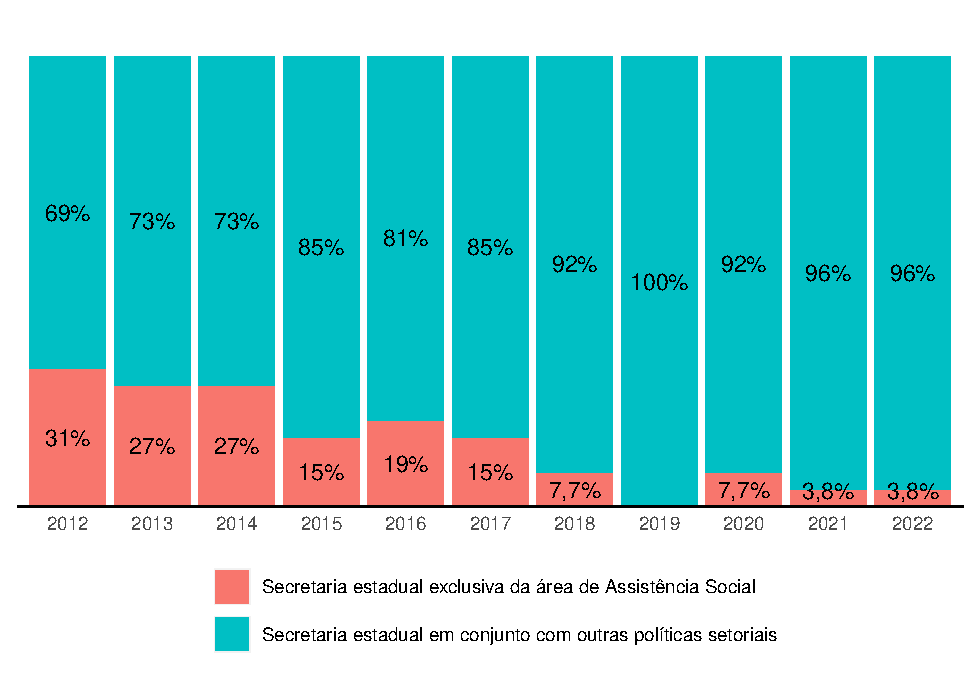
\includegraphics{Censo-SUAS-2022_files/figure-latex/estados_sec_exc-1} \caption[Percentual de Estados quanto a caracteristica de estrutura administrativa - Brasil, 2012 a 2022]{Percentual de Estados quanto a caracteristica de estrutura administrativa - Brasil, 2012 a 2022}\label{fig:estados_sec_exc}\floatfoot{Fonte: MDS, Censo SUAS}
\end{figure}

No que se refere aos municípios, esse cenário nacional se configurou
inverso ao das gestões Estaduais. Observa-se através do
\cref{fig:sec-munic-exc} um aumento de 217 municípios (1,5 pontos
percentuais) com secretarias exclusivas de Assistência Social do período
de 2012 a
2019\footnote{a partir de 2019 essa pergunta foi retirada do formulário de gestão municipal}.

\begin{figure}
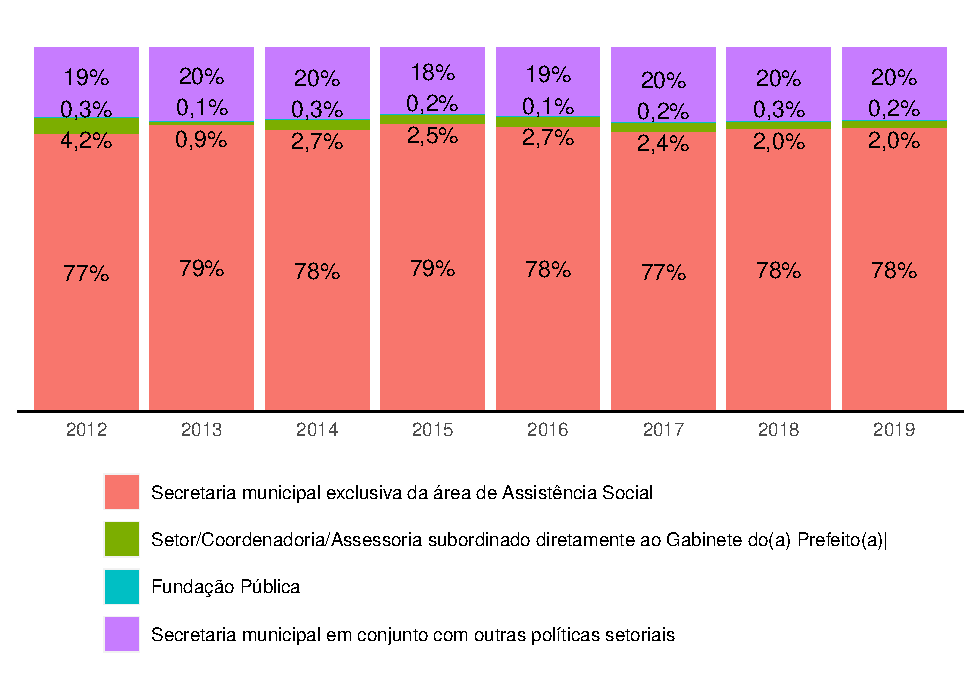
\includegraphics{Censo-SUAS-2022_files/figure-latex/sec-munic-exc-1} \caption[Percentual de Secretarias Municipais quanto a caracteristica de estrutura administrativa - Brasil, 2012 a 2019]{Percentual de Secretarias Municipais quanto a caracteristica de estrutura administrativa - Brasil, 2012 a 2019}\label{fig:sec-munic-exc}\floatfoot{Fonte: MDS, Censo SUAS}
\end{figure}

Alguns órgãos gestores estaduais constituíram as áreas de assistência
social como subdivisões administrativas em sua estrutura, como
superintendências, departamentos, gerências, coordenações, dentre
outras. De acordo com o último Pacto de aprimoramento Estadual do
SUAS\footnote{Resolução CNAS Nº2, de 16 de março de 2017} umas das
prioridades para o aperfeiçoamento institucional é possuir na estrutura
administrativa das seguintes areas:

\begin{enumerate}
\def\labelenumi{\arabic{enumi})}
\tightlist
\item
  Proteção Social Básica;
\item
  Proteção Social Especial de Média e Alta Complexidade;
\item
  Gestão do SUAS, com suas subdivisões de Vigilância Socioassistencial,
  Regulação do SUAS e Gestão do Trabalho; e
\item
  Gestão do Fundo Estadual de Assistência Social - FEAS.
\end{enumerate}

Observa-se avanço em todas as areas formalmente nos últimos 10 anos. As
três áreas mais instituídas são: Proteção Social Básica, Proteção Social
Especial com 88,46\% e Gestão do SUAS com 84,62\% (\Cref{fig:uf_subd}).

\begin{figure}
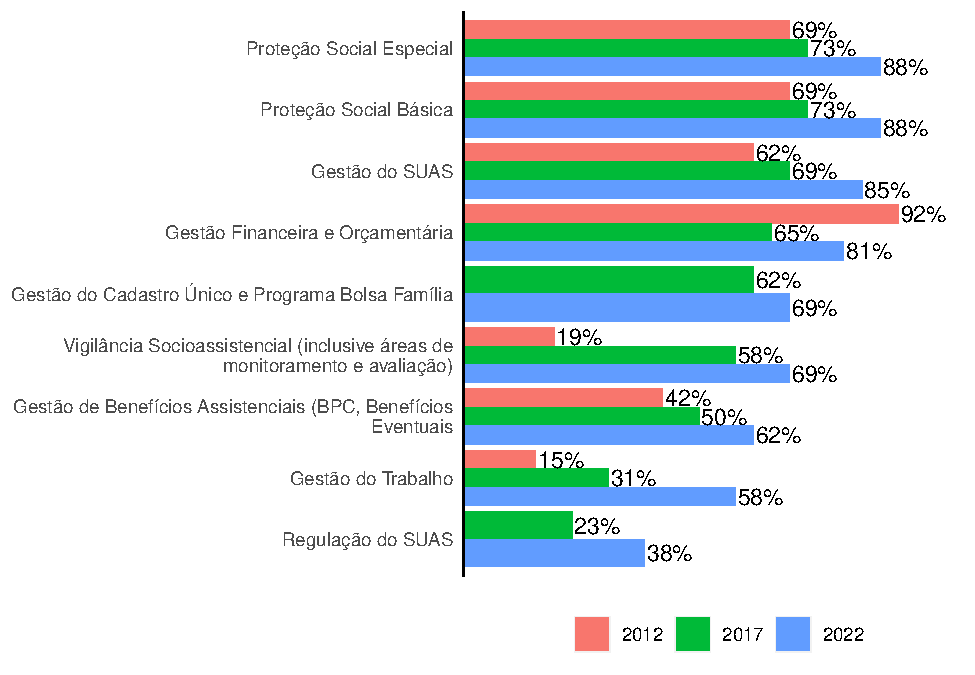
\includegraphics{Censo-SUAS-2022_files/figure-latex/uf_subd-1} \caption[Percentual de estados segundo subdivisões administrativas constituídas na estrutura formal do órgão gestor - Brasil]{Percentual de estados segundo subdivisões administrativas constituídas na estrutura formal do órgão gestor - Brasil; 2012, 2017 e 2022}\label{fig:uf_subd}\floatfoot{Fonte: MDS, Censo SUAS.}
\end{figure}

\begin{figure}
\includegraphics{Censo-SUAS-2022_files/figure-latex/uf_subd_constituidas-1} \caption[Percentual de estados segundo constituição de subdivisões administrativas na estrutura do órgão gestor - Brasil]{Percentual de estados segundo constituição de subdivisões administrativas na estrutura do órgão gestor - Brasil; 2012, 2017 e 2022}\label{fig:uf_subd_constituidas}\floatfoot{Fonte: MDS, Censo SUAS.}
\end{figure}

Quando se observa a regularização destas areas, há um grupo instituídas
informalmente conforme \cref{fig:estados-constituicao-subdivisoes}, e
setores que ainda não estão consituídos em 100\% dos estados, a saber
Gestão do SUAS, Gestão do trabalho e regulação do SUAS.

\begin{figure}
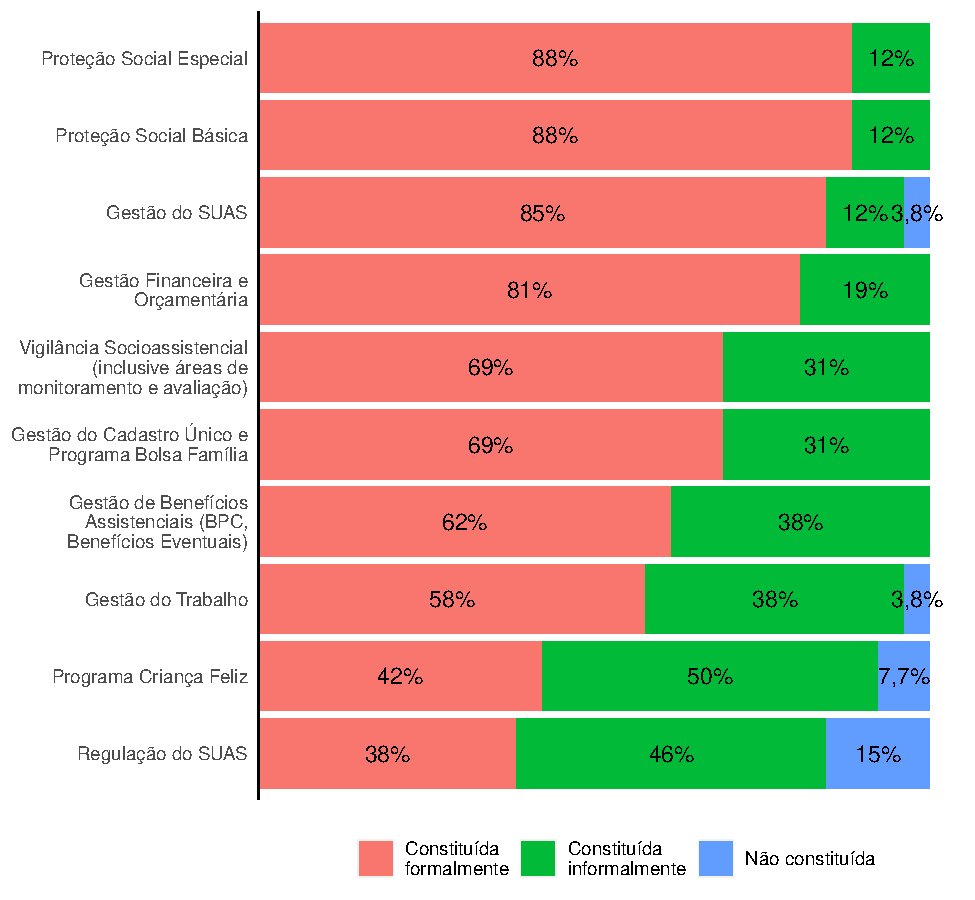
\includegraphics{Censo-SUAS-2022_files/figure-latex/estados-constituicao-subdivisoes-1} \caption[Percentual de estados segundo característica da estrutura administrativa da Secretaria Estadual de Assistência Social - Brasil,  2022]{Percentual de estados segundo característica da estrutura administrativa da Secretaria Estadual de Assistência Social - Brasil,  2022}\label{fig:estados-constituicao-subdivisoes}\floatfoot{Fonte: MDS, Censo SUAS.}
\end{figure}

No que se refere aos municípios, a última pactuação sobre estrutura
administrativa a partir dos portes populacionais dos
municípios\footnote{124ª reunião ordinária da CIT - Pacto de Aprimoramento do SUAS}
prevê:

\begin{itemize}
\item
  \textbf{municípios de pequeno I e II e médio porte:} 100\% dos
  municípios com instituição formal, na estrutura do órgão gestor de
  assistência social, as áreas constituídas de Proteção Social Básica,
  Proteção Social Especial e a área de Gestão do SUAS com competência de
  Vigilância Socioassistencial.
\item
  \textbf{municípios de grande porte e metrópole:} 100\% dos muncípios
  com instituição formal, na estrutura do órgão gestor de assistência
  social, áreas constituídas de Proteção Social Básica, Proteção Social
  Especial, com subdivisão de Média e Alta Complexidade, Gestão
  Financeira e Orçamentária, Gestão de Benefícios Assistenciais e
  Transferência de Renda, área de Gestão do SUAS com competência de:
  Gestão do Trabalho, Regulação do SUAS e Vigilância Socioassistencial.
\end{itemize}

O \cref{fig:munic_sub} mostra crescimento formal de todas as areas
administrativas. As areas do SUAS com maior percentual de constituição
formal\footnote{A regulamentação destas areas essenciais devem estar previstas no organograma. A Lei do SUAS Lei nº 12.435, de 06/07/2011 altera a Lei Organiza da Assistência Social (LOAS) - nº 8.742, de 07/.12.1993}
que dispõe sobre esta organização são respectivamente: Gestão do
Cadastro Único e Bolsa Família, Gestão da Proteção Social Básica e
Gestão do SUAS.

\begin{figure}
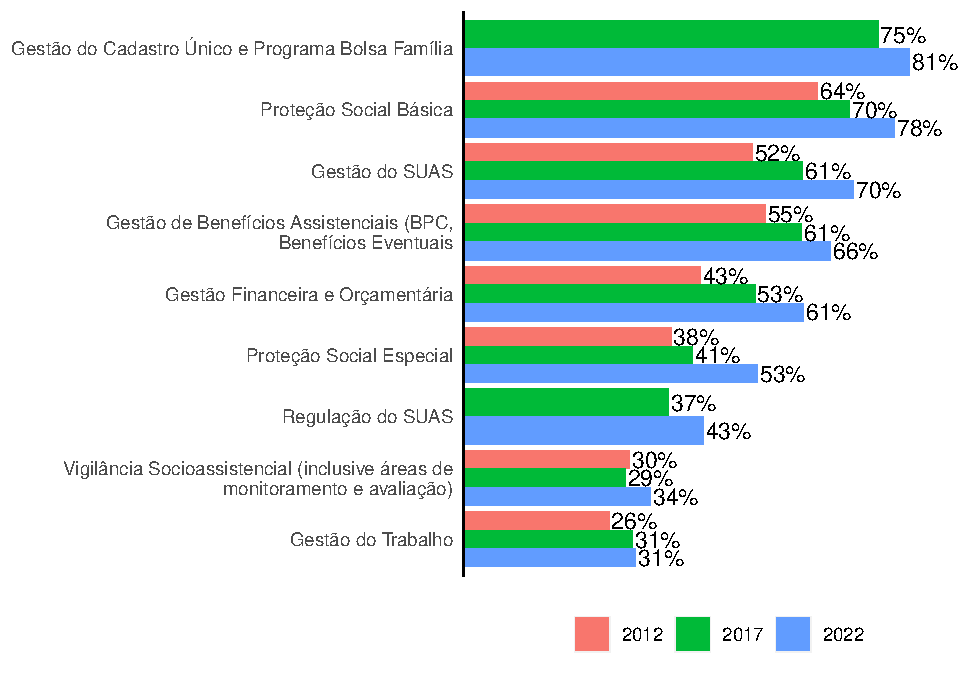
\includegraphics{Censo-SUAS-2022_files/figure-latex/munic_sub-1} \caption[Percentual segundo estrutura administrativa formal da Secretaria Municipal de Assistência Social - Brasil, 2012 - 2017 - 2022]{Percentual segundo estrutura administrativa formal da Secretaria Municipal de Assistência Social - Brasil, 2012 - 2017 - 2022}\label{fig:munic_sub}\floatfoot{Fonte: MDS, Censo SUAS.}
\end{figure}

Ao considerar a instituição informal, o
\cref{fig:municipais-constituicao-subdivisoes} sinaliza que a Gestão do
trabalho e Vigilância Socioassistencial são os mais altos percentuais de
informalidade e não constituição. Destaca-se também a proteção social
especial, area recomendada existir independe da presença de undiades de
CREAS.

\begin{figure}
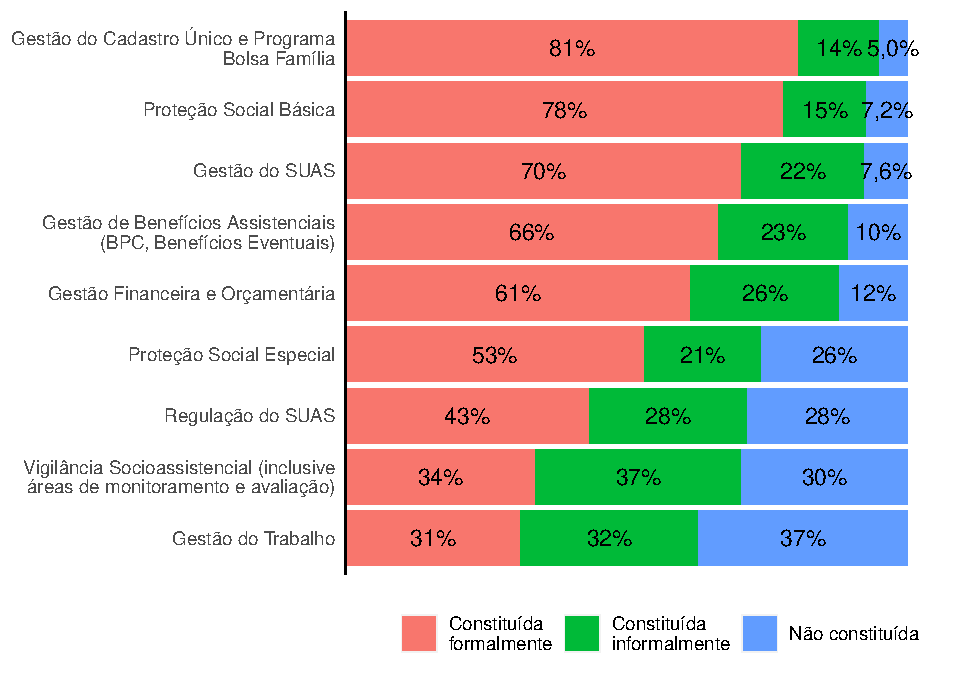
\includegraphics{Censo-SUAS-2022_files/figure-latex/municipais-constituicao-subdivisoes-1} \caption[Distribuição dos órgãos gestores municipais segundo constituição/formalização de subdivisões administrativas - Brasil, 2022]{Distribuição dos órgãos gestores municipais segundo constituição/formalização de subdivisões administrativas - Brasil, 2022}\label{fig:municipais-constituicao-subdivisoes}\floatfoot{Fonte: MDS, Censo SUAS}
\end{figure}

A uniformização da Lei do SUAS dos estados e municpípios em consonâcia
com a LOAS foi deliberação da X Conferência Nacional. Sobre essa
disposição, observa-se que nas gestões estaduais, 58\% dos estados
possuem Lei Estadual de regulamentação do SUAS (total de 15 estados). As
últimas atualizações ocorreram a partir de 2017 (12 estados), com
exceção de Minas Gerais em 2011 Goiás em 2015 e Mato Grosso do Sul em
2016.

Entratando, 11 estados que não possuem Lei do SUAS. Esse número estão
presentes nas seguintes regiões do Brasil: 4 - Nordeste, 3 - Norte, 2 -
Região Sul e 1 - Região Sudeste.
Sudeste\footnote{siglas dos Estado que não possuem Lei do SUAS - Censo SUAS 2022: RR, PA, TO, PI, RN, SE, BA, SP, PR, SC e RS}.

\begin{figure}
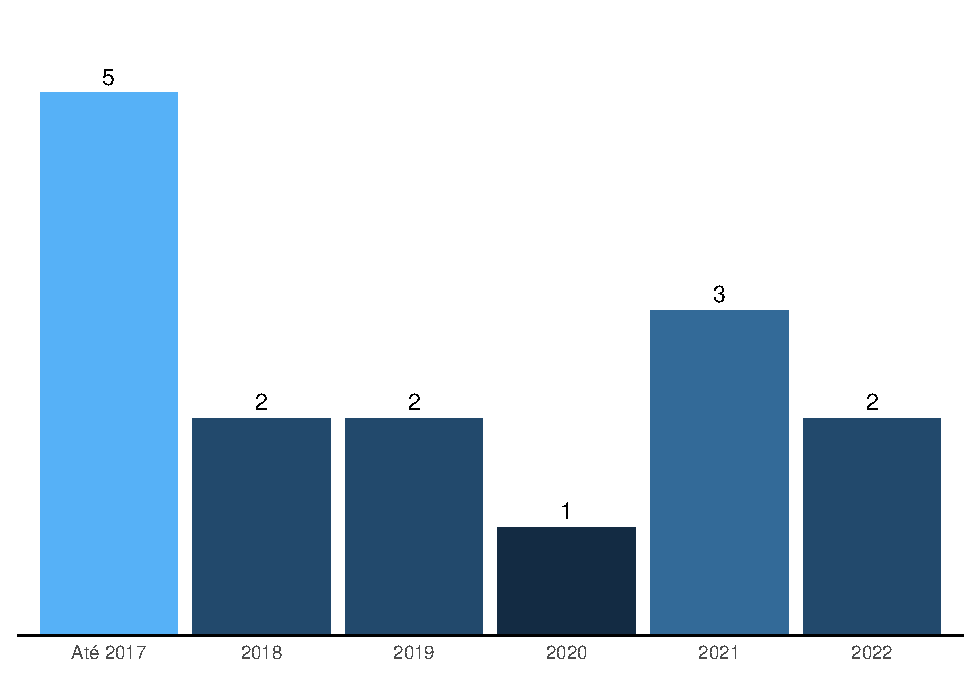
\includegraphics{Censo-SUAS-2022_files/figure-latex/estados-atualizacao-lei-1} \caption[Quantidade de estados segundo último ano de atualização da Lei Estadual de regulamentação do Sistema Único de Assistência Social (SUAS) - Brasil, 2022]{Quantidade de estados segundo último ano de atualização da Lei Estadual de regulamentação do Sistema Único de Assistência Social (SUAS) - Brasil, 2022}\label{fig:estados-atualizacao-lei}\floatfoot{Fonte: MDS, Censo SUAS.}
\end{figure}

Em 2022, 75\% dos municípios possuíam Lei Municipal de regulamentação do
SUAS (4.170). Destes, a maioria, 91\% (3.798) aprovaram/atualizaram após
2013 e 9\% (372) anterior a atualização da Lei
Nacional\footnote{Lei nº 12.435, de 06/07/2011 altera a Lei Organiza da Assistência Social (LOAS) - nº 8.742, de 07/.12.1993}
e a NOB SUAS/2012 conforme detalha o
\cref{fig:municipios-atualizacao-lei}. A inexistência de Lei é
encontrada em 25\% (1.400) dos municípios.

\begin{figure}
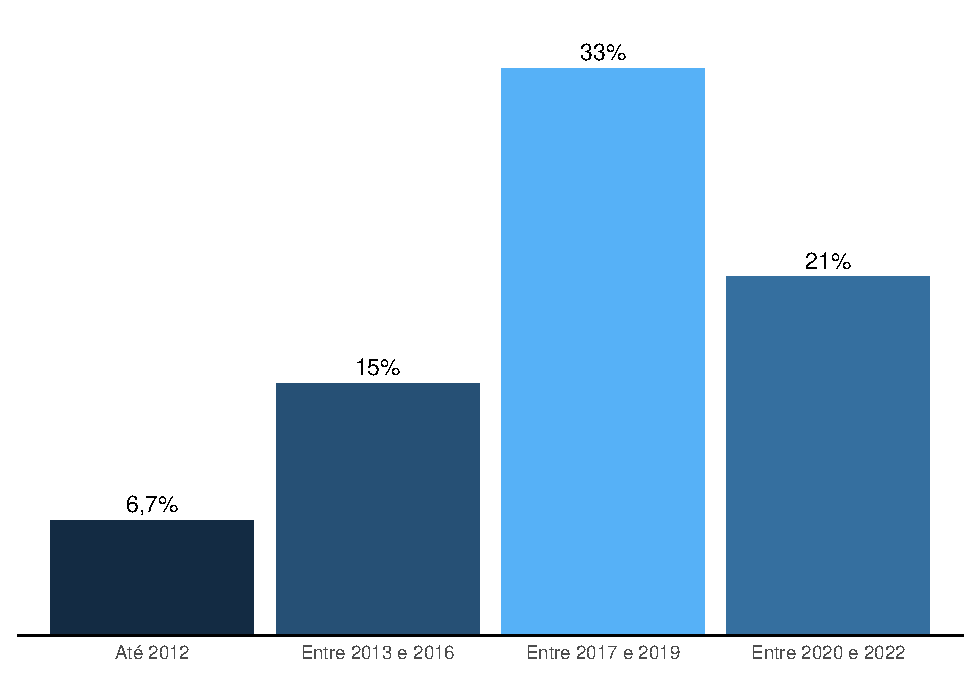
\includegraphics{Censo-SUAS-2022_files/figure-latex/municipios-atualizacao-lei-1} \caption[Percentual de municípios segundo último ano de atualização da Lei Municipal de regulamentação do Sistema Único de Assistência Social (SUAS) - Brasil, 2022]{Percentual de municípios segundo último ano de atualização da Lei Municipal de regulamentação do Sistema Único de Assistência Social (SUAS) - Brasil, 2022}\label{fig:municipios-atualizacao-lei}\floatfoot{Fonte: MDS, Censo SUAS.}
\end{figure}

No que se refere ao Planejamento, trata-se de uma obrigatoriedade para
existência do Sistema Único e repasse de confinanciamento. O Plano
Estadual de Assistência Social (PEAS) deve ser aprovado pelo Conselho
Estadual de Assistência Social (CEAS). Os dados do \cref{fig:PEAS}
sinalizam que a partir de 2020 há um descrecimo desta atualização com
devida aprovação do
conselho\footnote{Para os anos de 2016, 2017, 2018 e 2019 as perguntas alteraram, impossibilitande a linha histórica}\footnote{Para os municípios não foi possivel fazer essa linha histórica em decorrencia de mudanças nas perguntas}.

\begin{figure}
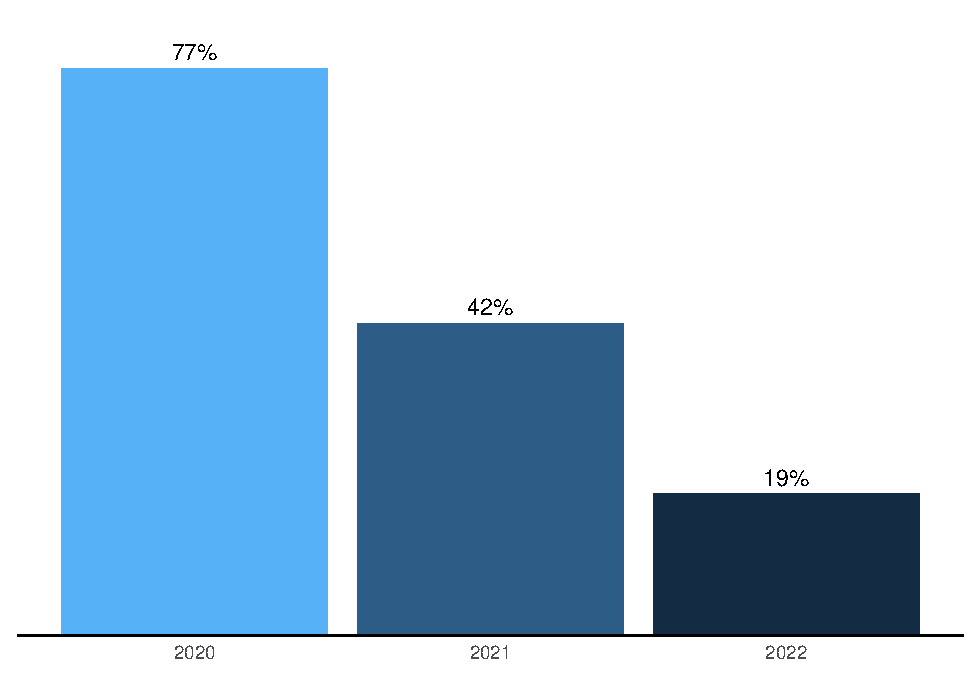
\includegraphics{Censo-SUAS-2022_files/figure-latex/PEAS-1} \caption[Percentual de Estados quanto a atualização do Plano Estadual de Assistência Social no ano do Censo - Brasil, 2020 a 2022]{Percentual de Estados quanto a atualização do Plano Estadual de Assistência Social no ano do Censo - Brasil, 2020 a 2022}\label{fig:PEAS}\floatfoot{Fonte: MDS, Censo SUAS}
\end{figure}

O Plano de apoio técnico aos municípios também é um produto a ser
realizado pelos Estados e previsto no último pacto de aprimoramento
Estadual do SUAS\footnote{Resolução CNAS Nº2, de 16 de março de 2017}.
De acordo com Censo Suas 2022, 57,69\% dos estados possuem este plano
pactuado na CIB. Este percentual reduziu em relação ao ano de 2017, na
qual mais de 76\% dos Estados informaram possuir este documento pactuado
nesta instância de comissão intergestores bipartite (CIB).

\begin{figure}
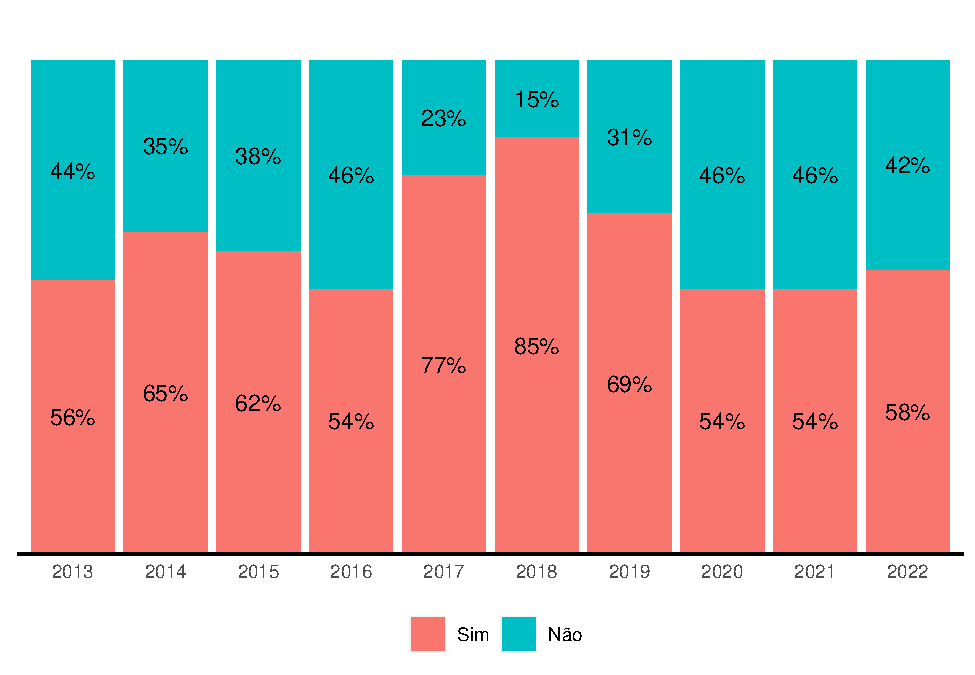
\includegraphics{Censo-SUAS-2022_files/figure-latex/plan_apoio_tec-1} \caption[Percentual de Estados que possuem Plano de Apoio Técnico pactuado na CIB - Brasil, 2013 a 2022]{Percentual de Estados que possuem Plano de Apoio Técnico pactuado na CIB - Brasil, 2013 a 2022}\label{fig:plan_apoio_tec}\floatfoot{Fonte: MDS, Censo SUAS}
\end{figure}

A NOB SUAS 2012 também evidencia o papel dos estados frente as
atribuições de apoio técnico e financeiro aos
municípios\footnote{Capítulo III - NOBSUAS/2012} na qual compreende
ações de:

\begin{enumerate}
\def\labelenumi{\Roman{enumi})}
\tightlist
\item
  Capacitação;
\item
  Elaboração de normas e instrumentos;
\item
  Publicação de materiais informativos e de orientações técnicas;
\item
  Assessoramento e acompanhamento;
\item
  Incentivos financeiros.
\end{enumerate}

Em 2022, todos os estados informaram realizar alguma modalidade de apoio
técnico aos municípios. Os maiores percentuais observados referiam-se ao
Apoio Técnico individualizado a municípios específicos ofertado por
96,2\% dos estados (25). Os menores percentuais eram referentes a
Seminários 46,2\%, (12). Outras formas eram ofertadas por 15,4\% dos
estados (\Cref{fig:estados-formas-apoio}).

Entre 2013 e 2022 o percentual de estados que prestavam assessoramento
técnico a distância aumentou significativamente, passando de 42,3\% (11)
em 2013 para 92,3\% (24) em 2022.

\begin{figure}
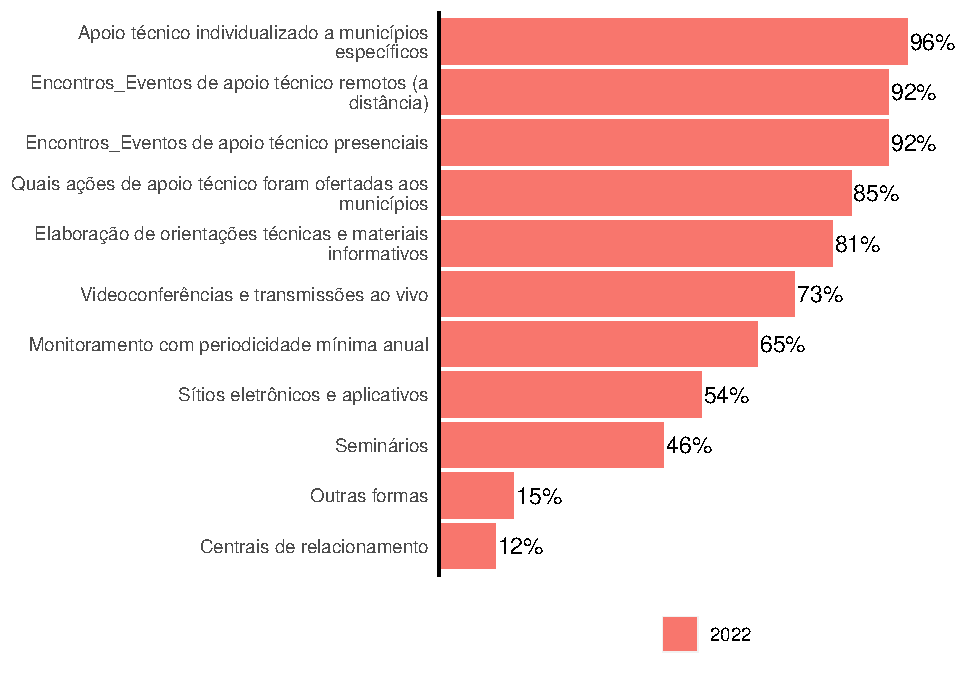
\includegraphics{Censo-SUAS-2022_files/figure-latex/estados-formas-apoio-1} \caption[Percentual de estados segundo formas de apoio técnico aos municípios - Brasil, 2022]{Percentual de estados segundo formas de apoio técnico aos municípios - Brasil, 2022}\label{fig:estados-formas-apoio}\floatfoot{Fonte: MDS, Censo SUAS.}
\end{figure}

No \cref{fig:munic_vit_estadual} os dados percentuais mostram um aumento
gradual dos municípios que informam receber visitas da gestão estadual
para apoio técnico. Entretanto 62,5\% informam não ter recebido visita
de apoio técnico no último ano.

\begin{figure}
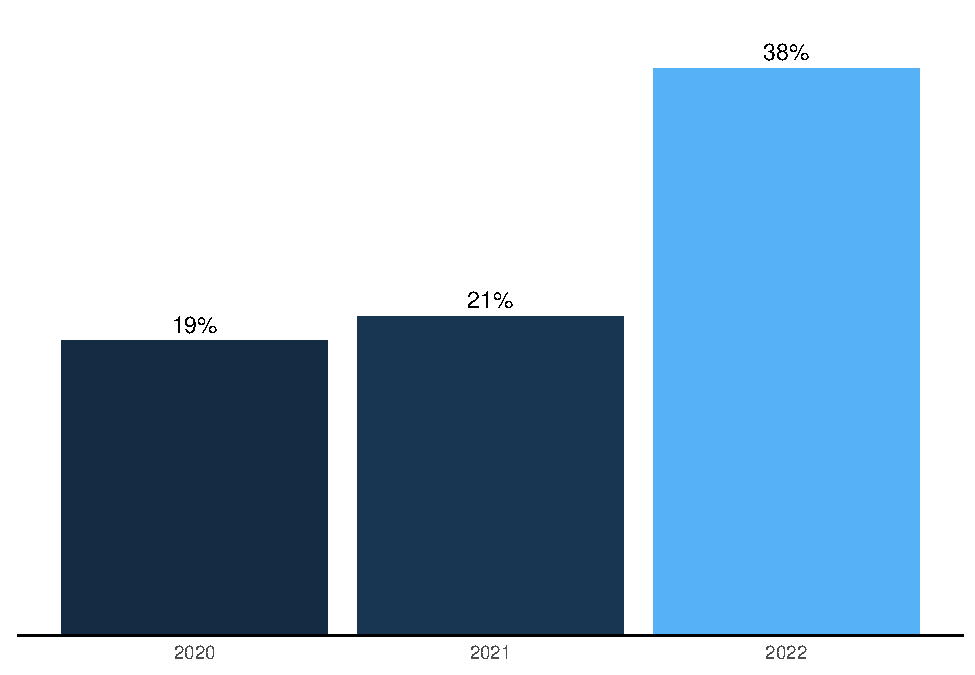
\includegraphics{Censo-SUAS-2022_files/figure-latex/munic_vit_estadual-1} \caption[Percentual de Municipios que informam receber visitas de Apoio Técnico do Estado - Brasil, 2020 a 2022]{Percentual de Municipios que informam receber visitas de Apoio Técnico do Estado - Brasil, 2020 a 2022}\label{fig:munic_vit_estadual}\floatfoot{Fonte: MDS, Censo SUAS}
\end{figure}

O modelo de gestão do SUAS preve cofinanciamento compartilhado entre os
três entes
federados\footnote{Art. 30-A.  O cofinanciamento dos serviços, programas, projetos e benefícios eventuais, no que couber, e o aprimoramento da gestão da política de assistência social no Suas se efetuam por meio de transferências automáticas entre os fundos de assistência social e mediante alocação de recursos próprios nesses fundos nas 3 (três) esferas de governo.}.

Nesta perspetiva, percebe-se um avanço nos últimos 10 anos sobre a
participação dos estados no cofinanciamento estadual com participação de
96,15\% (25) dos estados que informam cofinanciar os municípios
(\Cref{fig:estados-cofinanciamento-municipios}).

A forma de cofinanciamento deve ser viabilizada por meio de
transferência automática regular entre os fundos de assistência social
(Fundo a Fundo). Sobre esse item, observa-se que em 2012, 26,63\% (8)
dos estados realizavam cofinanciamento na modalidade de apenas Fundo a
Fundo e 25,9\% (7) apenas por convenio. Dado que avançou ao longo dos
anos, em 2022, 88,46\% (23) dos estados que realizam cofinanciamneto
regular e automático e nenhum estado apenas por convênio.

Apesar destes avanços, há registros de não cofinanciamento estadual, na
qual caiu de 25,93\% (7) no ano de 2012 para 3,85\% (1) em 2022
(1)\footnote{o Estado do Acre informa que não cofinancia os municípios}.

\begin{figure}
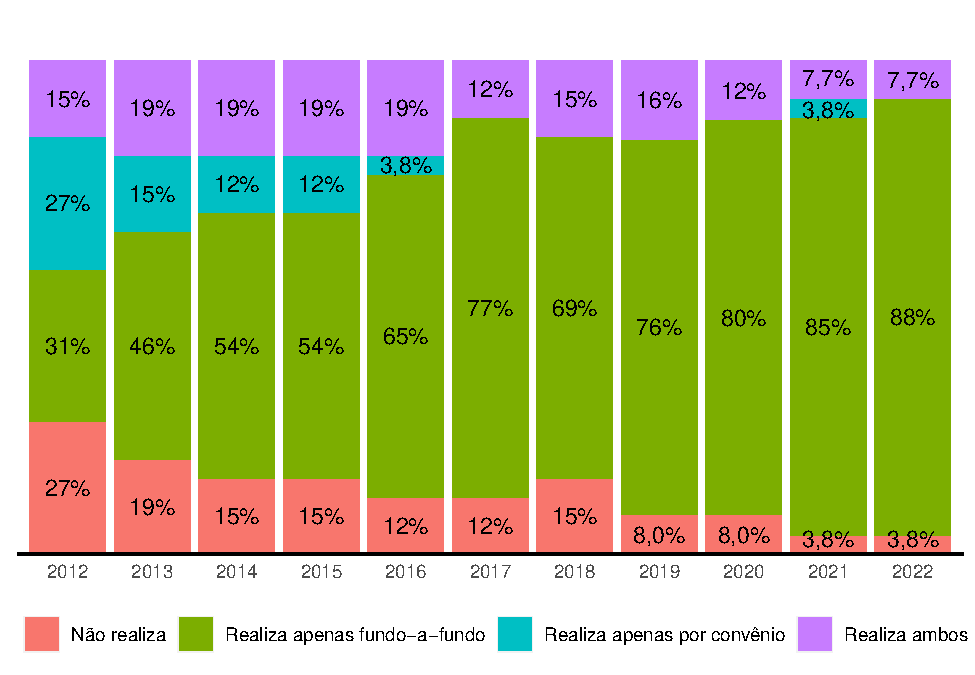
\includegraphics{Censo-SUAS-2022_files/figure-latex/estados-cofinanciamento-municipios-1} \caption[Percentual de estados segundo realização de cofinanciamento aos municípios - Brasil]{Percentual de estados segundo realização de cofinanciamento aos municípios - Brasil; 2012 a 2022}\label{fig:estados-cofinanciamento-municipios}\floatfoot{Fonte: MDS, Censo SUAS.}
\end{figure}

O \cref{fig:estados-blocos-recursos} evidencia a quantidade de estados
quando ao cofinanciamento aos municípios por blocos. Os dados dos
últimos 10 anos, sinaliza que o número de estados que cofinanciam os
municípios vem aumentando. Sobretudo o cofinanciamento da proteção
social especial (Média e Alta Complexoidade), em seguida Benefícios
Eventuais. No que se refere aos últimos 5 anos houve uma redução na
destinação de recursos para proteção social básica e incetivos do SUAS.

\begin{figure}
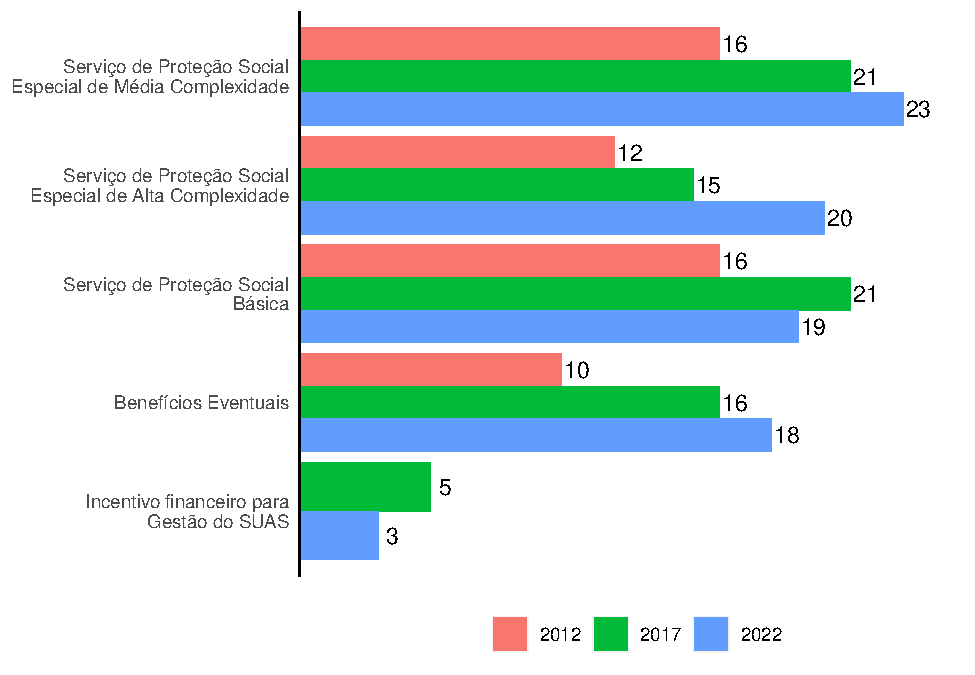
\includegraphics{Censo-SUAS-2022_files/figure-latex/estados-blocos-recursos-1} \caption[Número de estados segundo a destinação dos recursos transferidos aos municípios por blocos de financiamento - Brasil]{Número de estados segundo a destinação dos recursos transferidos aos municípios por blocos de financiamento - Brasil; 2012, 2017 e 2022}\label{fig:estados-blocos-recursos}\floatfoot{Fonte: MDS, Censo SUAS.}
\end{figure}

O ordenador de despesa responde pela emissão de empenho, autorização de
pagamento dos recursos do fundo de assistencia social. Assim,
recomenda-se que este tenha amplo conhecimento sobre a política. O
\cref{fig:estado_ord_despesa} sinaliza que 73\% dos gestores estaduais
são ordenadores de despesa do fundo estadual. Dado que reduziu a partir
de 2018.

\begin{figure}
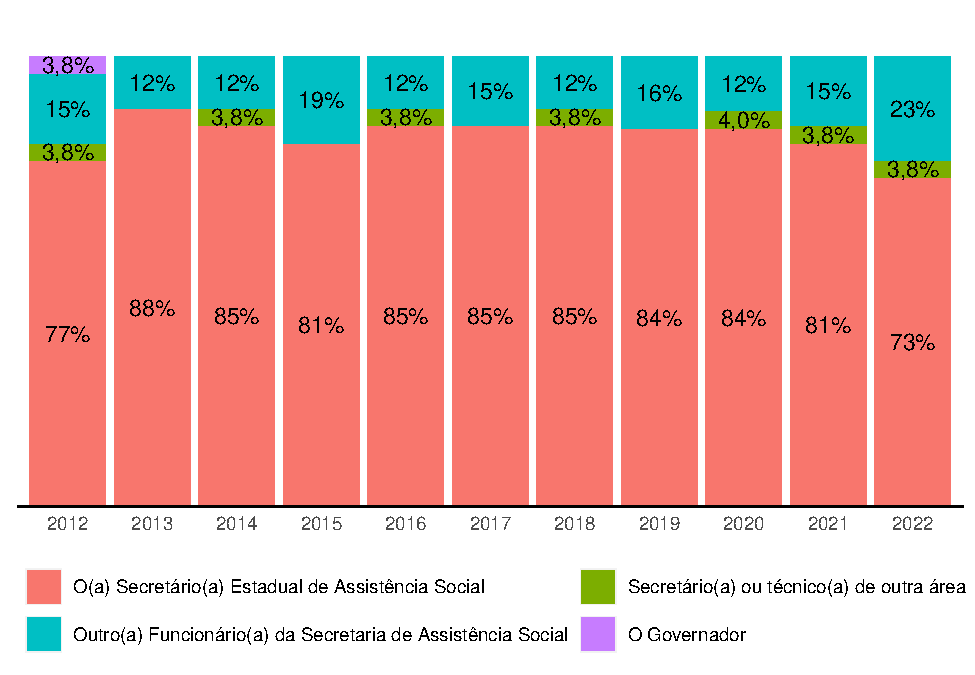
\includegraphics{Censo-SUAS-2022_files/figure-latex/estado_ord_despesa-1} \caption[Percentual de estados quanto a ordenação de despesa do Fundo Estadual - Brasil, 2018-2022]{Percentual de estados quanto a ordenação de despesa do Fundo Estadual - Brasil, 2018-2022}\label{fig:estado_ord_despesa}\floatfoot{Fonte: MDS, Censo SUAS.}
\end{figure}

No que se refere aos municípios, aproximadamente 80\% dos secretários
(as) municipais são ordenadores de despesa do Fundo Municipal. Esse
percentual aumentou a partir de 2016.

O \cref{fig:munic_ord_despesa} também mostra que as/os prefeitas/os
enquanto ordenadores de despesa da política de Assistência Social vem
reduzindo ao longo dos anos. Dado que se revela como positivo, haja
vista o gestor municipal encontra-se no cotidiano do planejamento desta
política pública, sendo mais apropriado para tomar as decisões sobre o
orçamento.

\begin{figure}
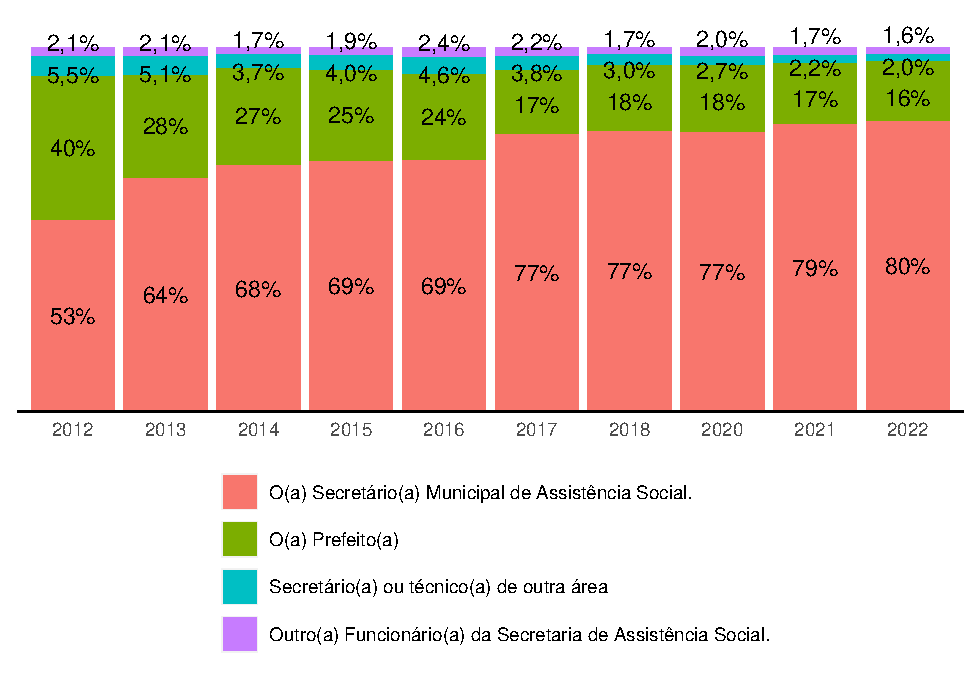
\includegraphics{Censo-SUAS-2022_files/figure-latex/munic_ord_despesa-1} \caption[Percentual de municípios quanto a ordenação de despesa do Fundo Municipal - Brasil, 2013 - 2022]{Percentual de municípios quanto a ordenação de despesa do Fundo Municipal - Brasil, 2013 - 2022}\label{fig:munic_ord_despesa}\floatfoot{Fonte: MDS, Censo SUAS.}
\end{figure}

No que se refere a Educação Permanente, nota-se um aumento dos estados
que possuem Núcleo de Educação Permante (\Cref{fig:NUEP}).

O censo de 2022 sinaliza 88,5\% (23) dos Estados possuem esta instancia
colegiada de maneira formal. Trata-se de um foro contituída pela
participação e cooperação institucionalizada de gestores, trabalhadores,
usuários, conselheiros de assistência social, e instituições de ensino,
pesquisa e extensão. O objetivo é deliberar sobre a implementação
continuada da Política de educação permanente do SUAS.

\begin{figure}
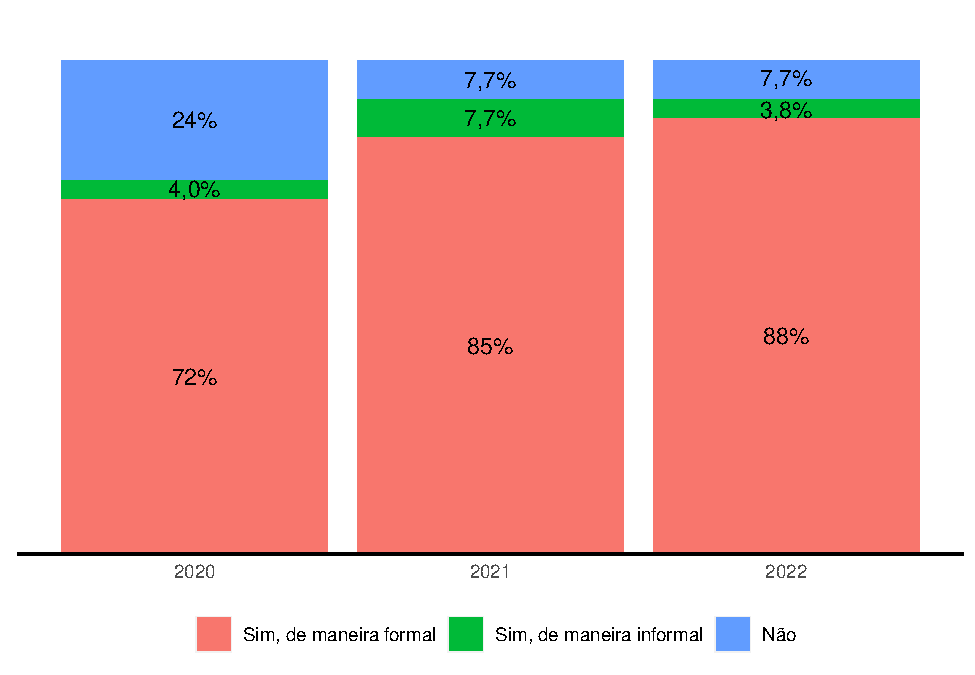
\includegraphics{Censo-SUAS-2022_files/figure-latex/NUEP-1} \caption[Percentual de Estados que possuem Núcleo de Educação Permanente, 2020 a 2022]{Percentual de Estados que possuem Núcleo de Educação Permanente, 2020 a 2022}\label{fig:NUEP}\floatfoot{Fonte: MDS, Censo SUAS}
\end{figure}

Em relação ao Plano de Educação Permanente, de acordo com censo suas de
2021, 13,9\% (769) dos municípios possuem este plano. Esse percentual,
como pode ser observado no \cref{fig:PNEP_Munic}, teve evolução residual
últimos anos\footnote{Para o ano de 2022 essa pergunta foi extinta}.

\begin{figure}
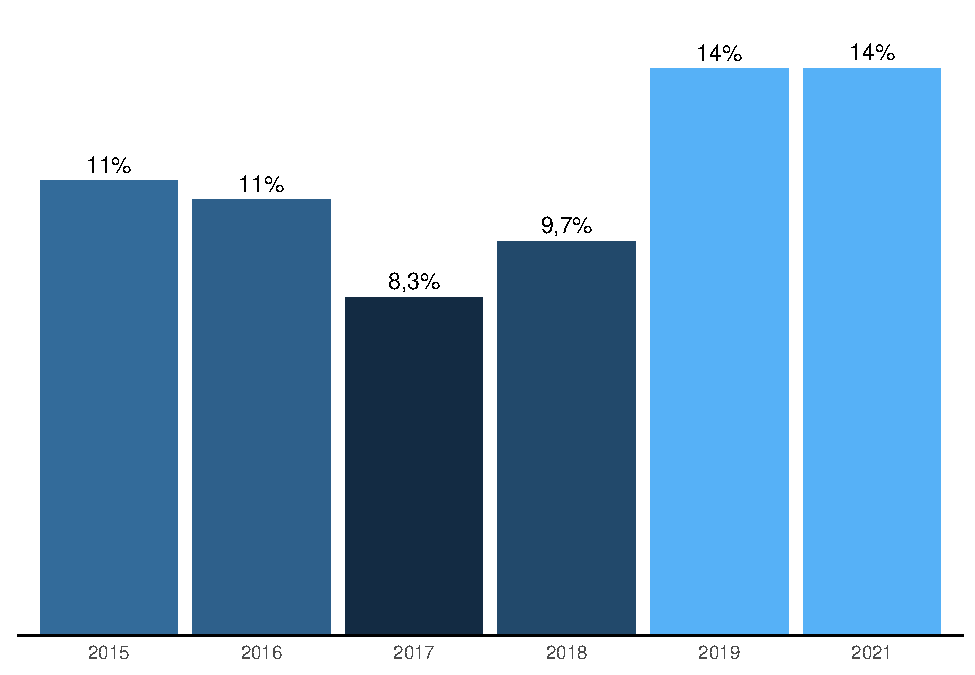
\includegraphics{Censo-SUAS-2022_files/figure-latex/PNEP_Munic-1} \caption[Percentual de municípios que possuem Plano de Capacitação e Educação Permanente, - Brasil]{Percentual de municípios que possuem Plano de Capacitação e Educação Permanente, - Brasil; 2015, 2017 e 2022}\label{fig:PNEP_Munic}\floatfoot{Fonte: MDS, Censo SUAS}
\end{figure}

\hypertarget{programas-de-execuuxe7uxe3o-pruxf3pria-executadas-pelos-estados}{%
\section{Programas de execução própria executadas pelos
estados}\label{programas-de-execuuxe7uxe3o-pruxf3pria-executadas-pelos-estados}}

Em relação aos programas próprios de transferência de renda executados
pelos estados, percebe-se um aumento ao longo dos anos na qual em 2022,
65\% dos estados informaram que possuem conforme o
\cref{fig:be_uf_renda}.

\begin{figure}
\includegraphics{Censo-SUAS-2022_files/figure-latex/be_uf_propria-1} \caption[Percentual de estados que possuem programas de execução própria]{Percentual de estados que possuem programas de execução própria}\label{fig:be_uf_propria}\floatfoot{Fonte: MDS, Censo SUAS}
\end{figure}
\begin{figure}
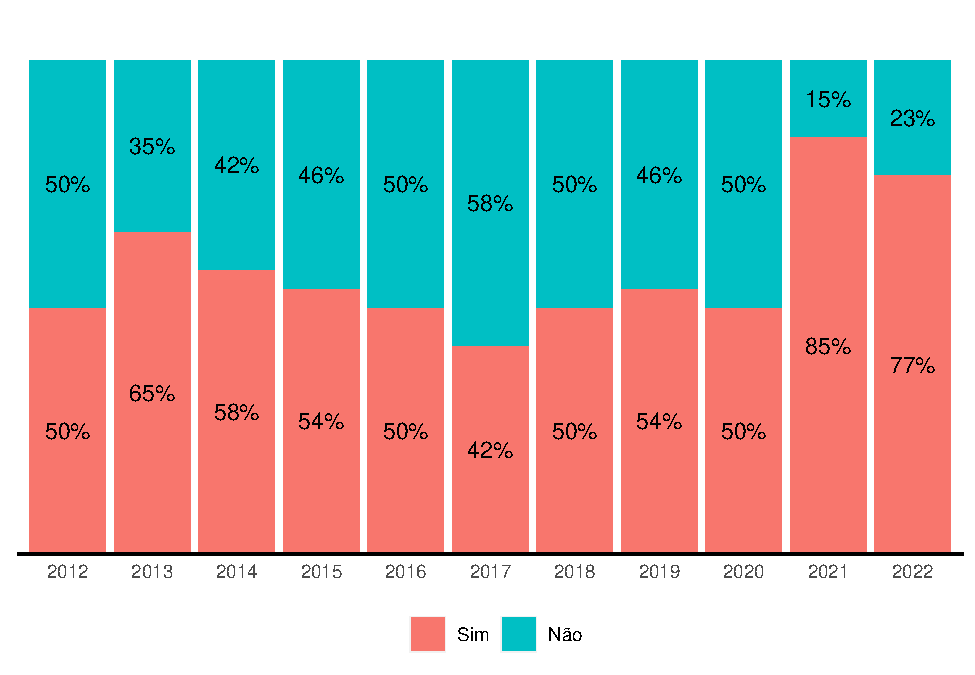
\includegraphics{Censo-SUAS-2022_files/figure-latex/be_uf_renda-1} \caption[Percentual de estados que possuem programa próprio de transferência de renda]{Percentual de estados que possuem programa próprio de transferência de renda}\label{fig:be_uf_renda}\floatfoot{Fonte: MDS, Censo SUAS}
\end{figure}

O Cadastro Único é ferramenta que possibilita inserção a programas
sociais no ambito dos três entes, o grafico abaixo sinaliza evolução dos
estados que usam o cadastro único enquanto respostas de programas
estaduais.

\begin{figure}
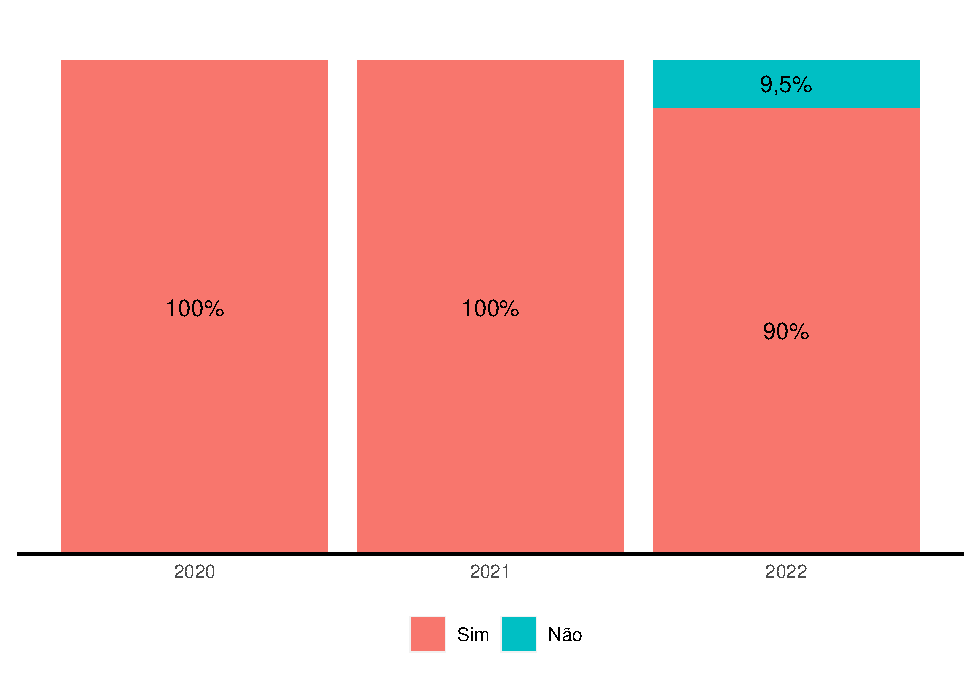
\includegraphics{Censo-SUAS-2022_files/figure-latex/uf_usa_cad-1} \caption[Percentual de estados que possuem programas de execução própria utilizando o Cadastro Único para seleção dos beneficiários]{Percentual de estados que possuem programas de execução própria utilizando o Cadastro Único para seleção dos beneficiários}\label{fig:uf_usa_cad}\floatfoot{Fonte: MDS, Censo SUAS}
\end{figure}

\section[Gestão do Cadastro Único]{Gestão do Cadastro Único\footnote{O formulário do posto do cadastro único foi criado em 2020, assim a maioria das informações disponíveis terão referencia esta data.}}

O Cadastro Único para Programas Sociais do Governo Federal (Cadastro
Único) instituído por meio do art. 6º-F da Lei nº 8.742, de 7 de
dezembro de 1993 (Lei Orgânica da Assistência Social), e regulamentado
por meio do Decreto nº 11.016, de 29 de março de 2022 tem a finalidade
de coletar, sistematizar e disseminar informações que permitem a
identificação e caracterização das condições socioeconômicas das
famílias em situação de vulnerabilidade social, sobretudo para as
famílias de baixa de renda.

O objetivo é conhecer, incluir e aprimorar as políticas sociais através
do acesso a Serviços, Programas, benefícios, identificação das famílias
e territórios vulnerabilizados, bem como ações intersetoriais.

A gestão do Cadastro Único é compartilhada entre união, estados,
municípios e distrito federal na qual cabe aos estados o apoio técnico,
capacitação, monitoramento e avaliação. É nos municípios que estão os
locais de cadastramento e toda gestão territorial da identificação das
famílias neste cadastro público.

As unidades do Cadastro Único podem ser encontradas em locais exclusivos
ou na rede de atendimento socioassistencial de CRAS, CREAS, Centro Pop.
Dados do Censo SUAS mostram uma evolução de locais de cadastramento,
sobretudo a partir de 2017.

Sobre a distribuição destes locais de Cadastro Único, destaca-se que em
2022, 31\% (2.892) são unidades exclusivas de Cadastro Único e 68\%
estão em unidades da rede
socioassistencial\footnote{CRAS, CREAS e CENTRO POP} conforme pode ser
observado na tabela \ref{tab:qtd_unidades}.

\begin{table}[H]
\centering
\caption{Quantidade de Unidades de Cadastro Único}
\label{tab:qtd_unidades}
\begin{tabular}{@{}lcccccc@{}}
\toprule
Unidades             & 2017  & 2018 & 2019 & 2020 &  2021 & 2022            \\ \midrule
CRAS                    & 5.669 & 5.508 & 5.923 & 5.729 & 5.937 & 6.090         \\
CREAS                   & 281 & 174 & 199 & 199 & 208 & 230                     \\
Centro POP              & 112 & 83 & 84 & 108 & 106 & 115                       \\
Postos Cadastro Único   & - & - & - & 2.530 & 2.695 & 2.892                       \\ \bottomrule
\textbf{Total}                   &\textbf{6.062} & \textbf{5.765} & \textbf{6.206} & \textbf{8.566} & \textbf{8.946} & \textbf{9.327}          \\ \bottomrule
\end{tabular}
\floatfoot{Fonte: MDS, Censo SUAS.}
\end{table}

A respeito da estrutura física das unidades exclusivas do Cadastro Único
destacadas acima, 61,0\% encontram-se na sede da Secretaria de
Assistência Social e 24,3\% em estruturas especificas. Os demais
percentuais são encontrados em outra unidade administrativa como, em um
serviço integrado, OSC´s, conselho ou escola.

No que se refere a gestão territorial, cabe as coordenações do Cadastro
Único dos municípios o atendimento, a supervisão, o monitoramento e a
avaliação dos processos de cadastramento, seja em postos específicos ou
integradas as unidades da rede socioassistencial.

O \cref{fig:gestao_cad} sinaliza que, no âmbito da gestão municipal, as
ações de levantamento de famílias para atualização e inclusão cadastral
são a mais realizada. A menor proporção se refere a ações de elaboração
de análises utilizando dados do Cadastro Único
(\Cref{fig:gestao_cad})\footnote{estas informações são do formulário de Gestão Municipal, assim se referem a informações gerais que a gestão informa realizar, destaca-se também que estas informações estão disponíveis a partir do ano de 2020}.

\begin{figure}
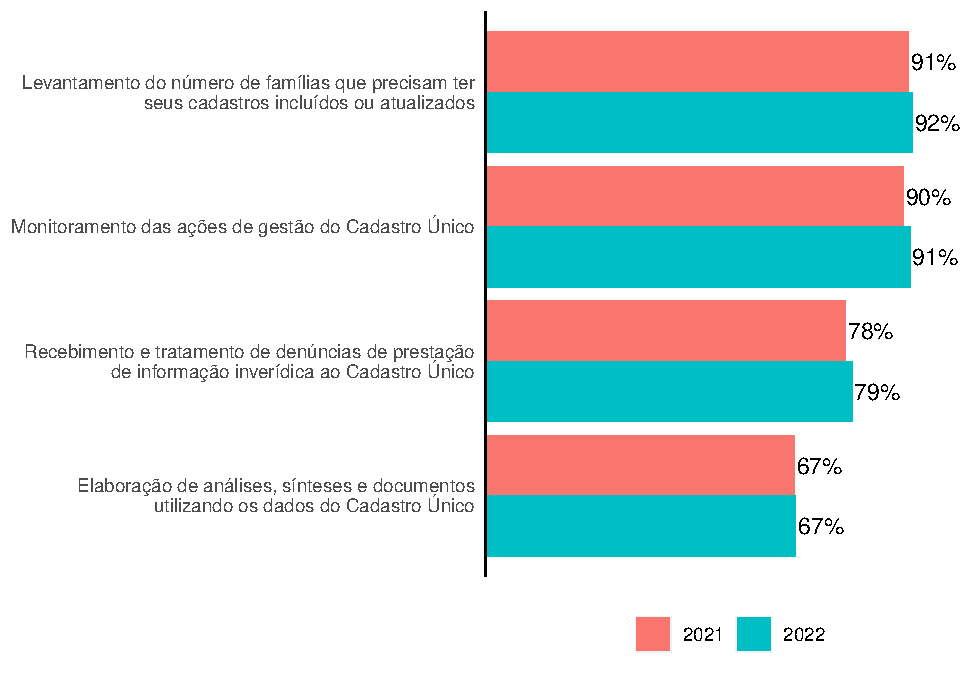
\includegraphics{Censo-SUAS-2022_files/figure-latex/gestao_cad-1} \caption[Ações desenvolvidas no âmbito da Gestão do Cadastro Único - Brasil, 2021 e 2022]{Ações desenvolvidas no âmbito da Gestão do Cadastro Único - Brasil, 2021 e 2022}\label{fig:gestao_cad}\floatfoot{Fonte: MDS, Censo SUAS.}
\end{figure}

O \cref{fig:acoes_cad} sinaliza que as ações de esclarecimento de
dúvidas sobre serviços, programas entre outros são realizadas pela
grande maioria das unidades do cadastro único (96,82\%). Já as ações de
agendamento para atendimento são realizadas por 64,35\% das unidades,
com redução ao longo dos
anos\footnote{estas informações são dos postos que executam exclusivamente atividades do cadastro único}.

\begin{figure}
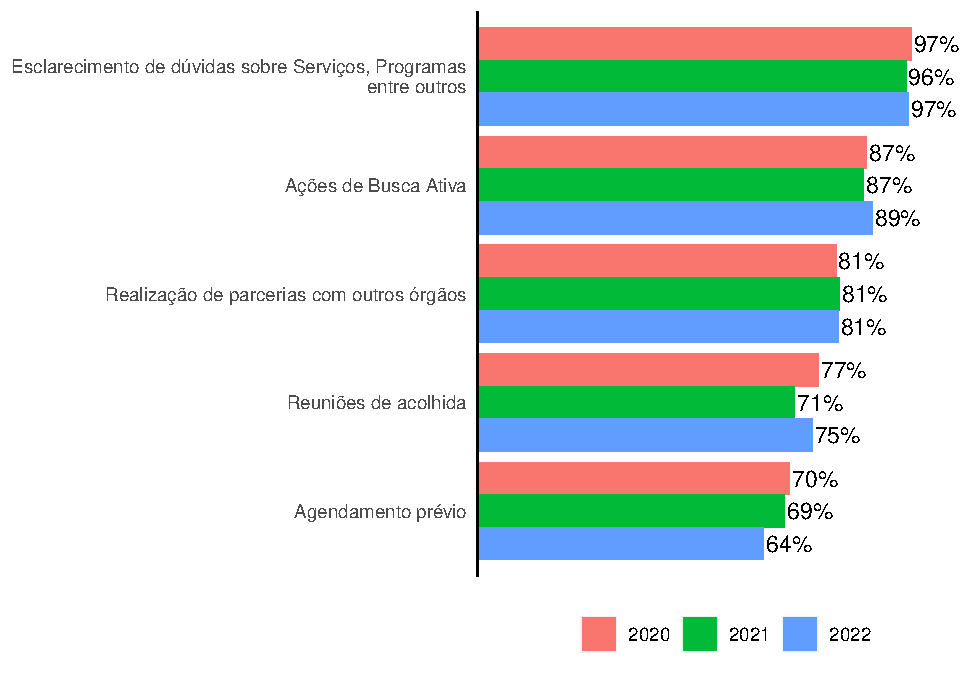
\includegraphics{Censo-SUAS-2022_files/figure-latex/acoes_cad-1} \caption[Ações desenvolvidas pelos postos do Cadastro Único - Brasil, 2020, 2021 e 2022]{Ações desenvolvidas pelos postos do Cadastro Único - Brasil, 2020, 2021 e 2022}\label{fig:acoes_cad}\floatfoot{Fonte: MDS, Censo SUAS.}
\end{figure}

Faz parte de procedimentos de qualificação do Cadastro Único ações de
averiguação e revisão cadastral. A averiguação é um processo de
verificação das informações registradas no Cadastro Único por meio da
comparação dos dados declarados pelas famílias com outros dados e
registros administrativos do governo federal. Já a revisão é um
procedimento de atualização das famílias com registros desatualizados. O
tempo considerado para um cadastro desatualizado é de 24 meses. O
\cref{fig:ave_cad} refere-se as informações de averiguação e revisão
cadastral no âmbito dos postos dos Cadastro Único dos municípios.
Nota-se que ao longo dos anos, essas ações aumentaram,sobretudo as ações
de busca ativa e identificação do público de averiguação e revisão
cadastral como público prioritário.

\begin{figure}
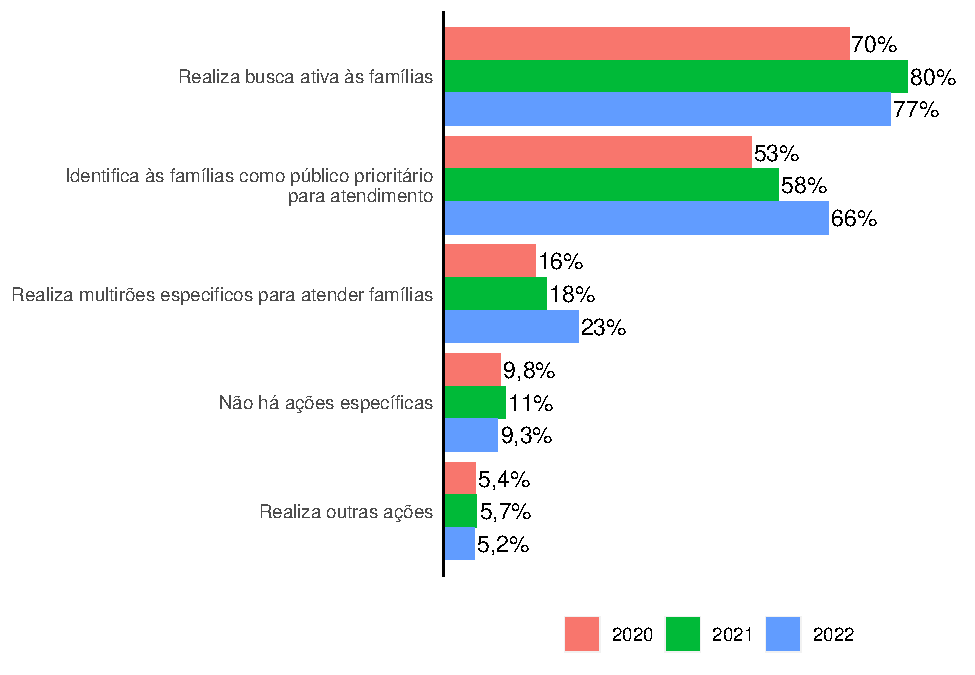
\includegraphics{Censo-SUAS-2022_files/figure-latex/ave_cad-1} \caption[Ações de averiguação e revisão desenvolvidas pelas Unidades do Cadastro Único - Brasil, 2020, 2021 e 2022]{Ações de averiguação e revisão desenvolvidas pelas Unidades do Cadastro Único - Brasil, 2020, 2021 e 2022}\label{fig:ave_cad}\floatfoot{Fonte: MDS, Censo SUAS.}
\end{figure}

Em relação as informações de unidades de Postos do Cadasto Único e o
atendimento de Grupos Populacionais Tradicionais e Específicos - GPTEs,
destaca-se através do \cref{fig:gptes-cadunico} o percentual de unidades
de postos do Cadastro Único que informam atender no período de 2020 a
2022.

\begin{figure}
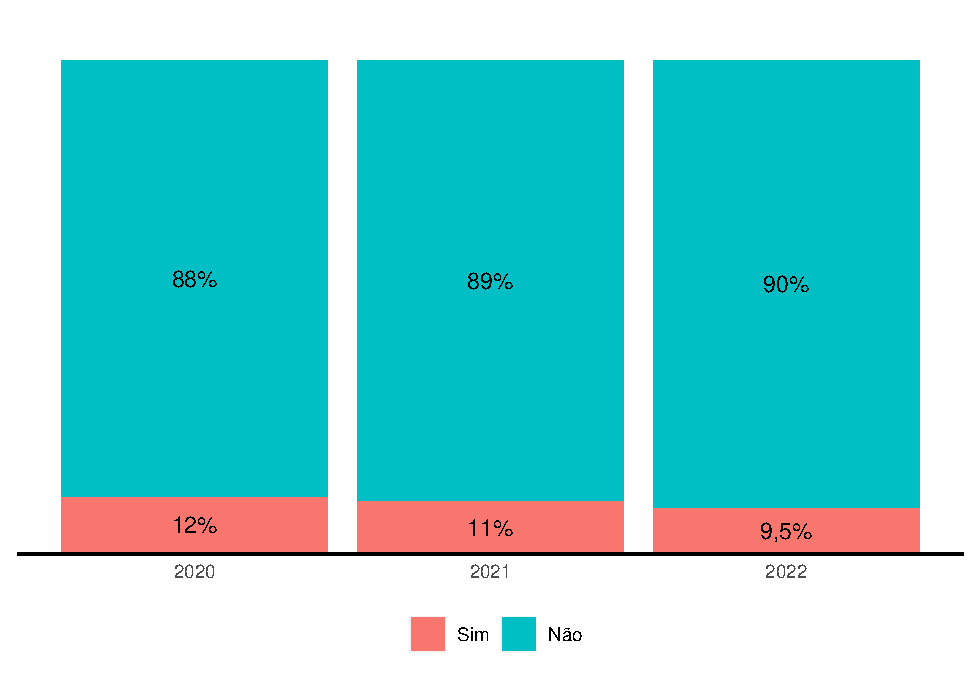
\includegraphics{Censo-SUAS-2022_files/figure-latex/gptes-cadunico-1} \caption[Unidades que realizam cadastramento de famílias pertencentes a Grupos Tradicionais e Específicos (GPTEs) - Brasil, 2020 a 2022]{Unidades que realizam cadastramento de famílias pertencentes a Grupos Tradicionais e Específicos (GPTEs) - Brasil, 2020 a 2022}\label{fig:gptes-cadunico}\floatfoot{Fonte: MDS, Censo SUAS}
\end{figure}

O cadastramento domiciliar permite uma aproximação com aspectos do
cotidiano das famílias, visto que a coleta das informações ocorre por
meio do encontro da gestão até as famílias. Essa ação objetiva assegurar
o acesso a inclusão ou atualização cadastral na residencia das pessoas.
De acordo com informações do \cref{fig:visit_dom} as situações mais
frequentes para visita domiciliar são para averiguação cadastral e
inclusão/atualização de dados do BPC (Benefício de Prestação Continuada
- BPC).

\begin{figure}
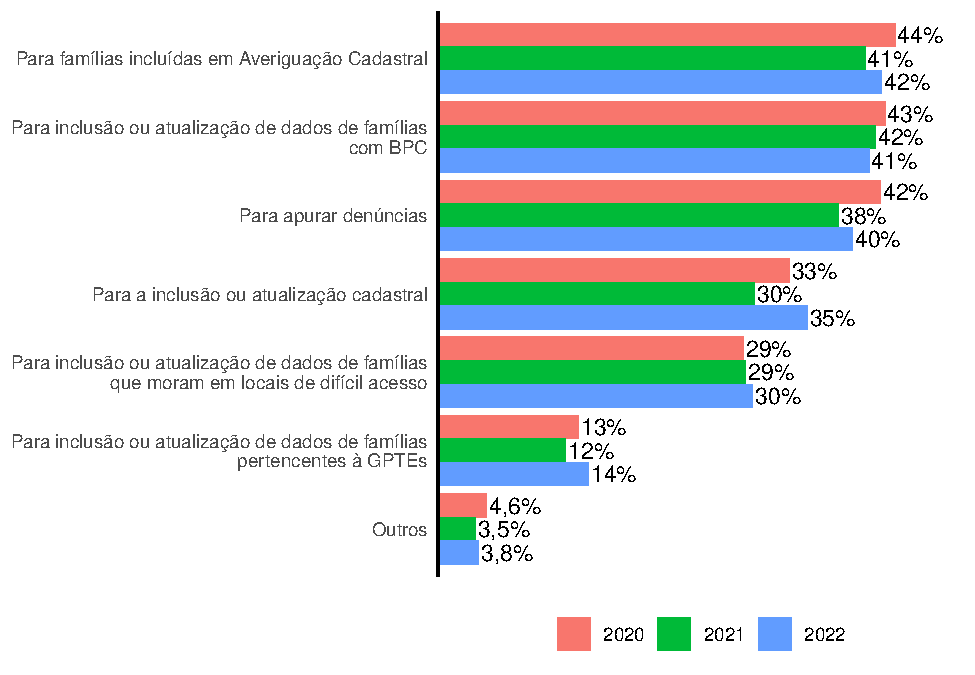
\includegraphics{Censo-SUAS-2022_files/figure-latex/visit_dom-1} \caption[Situações mais frequentes de entrevistas domiciliares no Cadastro Único - Brasil, 2020, 2021 e 2022]{Situações mais frequentes de entrevistas domiciliares no Cadastro Único - Brasil, 2020, 2021 e 2022}\label{fig:visit_dom}\floatfoot{Fonte: MDS, Censo SUAS.}
\end{figure}

Em relação as ações de complementariedade com a rede socioassistencial,
destaca-se que a maioria destas unidades de cadastramento realizam
encaminhamentos para rede socioassistencial de CRAS, CREAS, Centro Pop
entre outros (\Cref{fig:redesuas}).

\begin{figure}
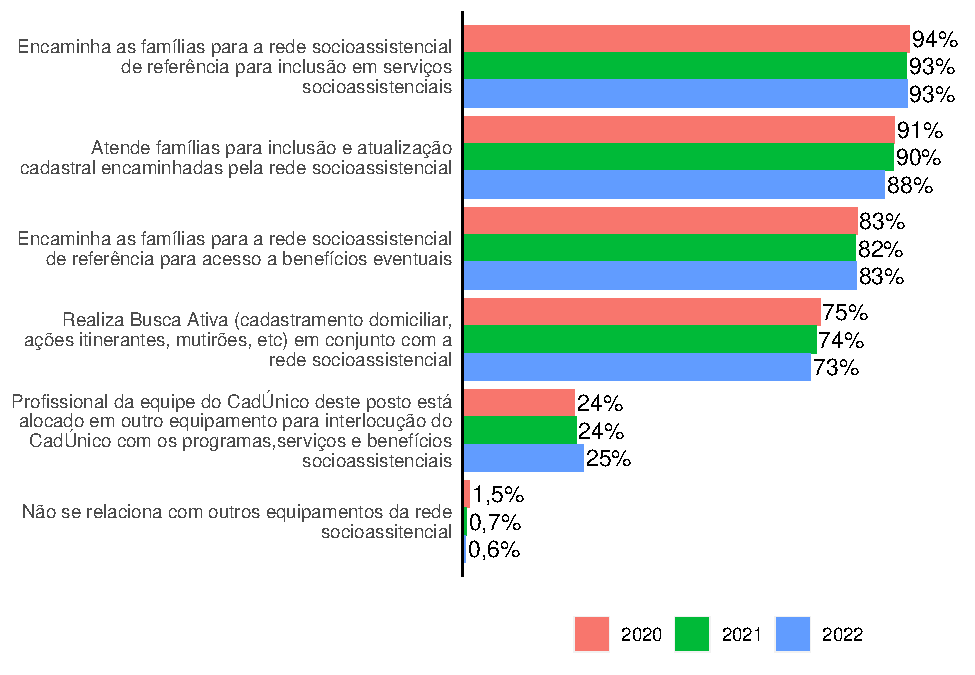
\includegraphics{Censo-SUAS-2022_files/figure-latex/redesuas-1} \caption[Percentual de postos de Cadastro Único segundo relação com os outros equipamentos da rede socioassistencial - Brasil, 2020, 2021 e 2022]{Percentual de postos de Cadastro Único segundo relação com os outros equipamentos da rede socioassistencial - Brasil, 2020, 2021 e 2022}\label{fig:redesuas}\floatfoot{Fonte: MDS, Censo SUAS.}
\end{figure}

O \cref{fig:igdbolsa} sinaliza sobre a existência da participação das
unidades do Cadastro único no planejamento dos recursos recebidos no
âmbito do IGD-PBF (Índice de Gestão Descentralizada da Gestão do Bolsa
Família e Cadastro Único).

Trata-se de um recurso repassado aos estados e municípios para apoio a
gestão do Cadastro Único e Bolsa Família. Esta informação é referente a
respostas do dormulário dos potos de cadastramento em âmbito dos
municípios.

\begin{figure}
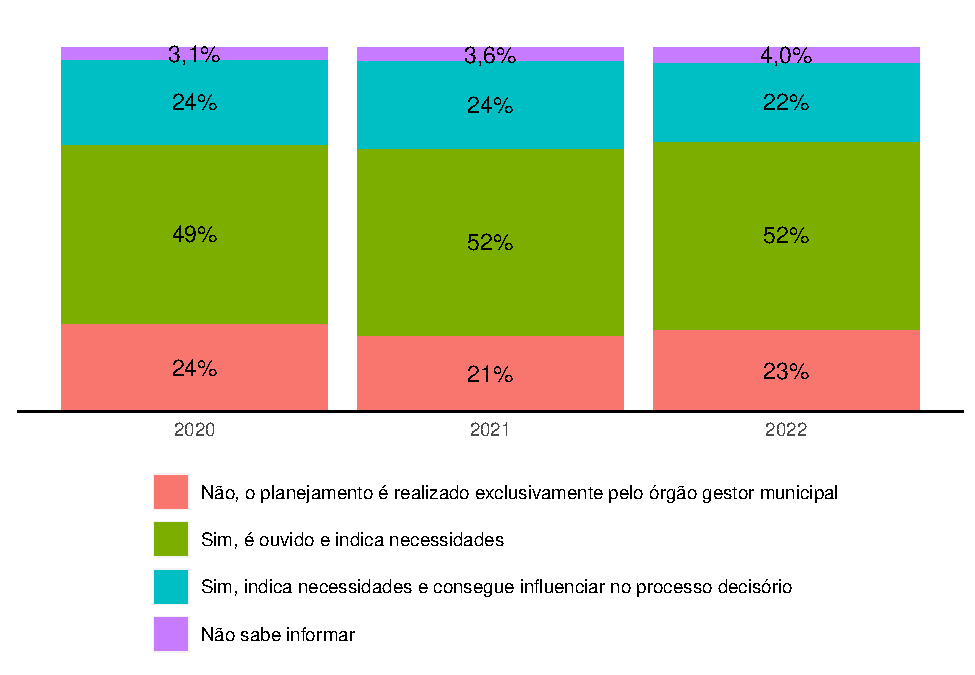
\includegraphics{Censo-SUAS-2022_files/figure-latex/igdbolsa-1} \caption[Unidades de Postos do Cadastro Único quanto a participação no planejamento do IGD Bolsa Família - Brasil, 2020 - 2021 - 2022]{Unidades de Postos do Cadastro Único quanto a participação no planejamento do IGD Bolsa Família - Brasil, 2020 - 2021 - 2022}\label{fig:igdbolsa}\floatfoot{Fonte: MDS, Censo SUAS}
\end{figure}

Em relação a existência de coordenador(a) do Cadastro Único nos postos
de atendimento, o \cref{fig:coord_cadunico} sinaliza aumento nos últimos
anos, em 2022, 31,8\% dos postos do Cadastro Único possuem
coordenador(a).

\begin{figure}
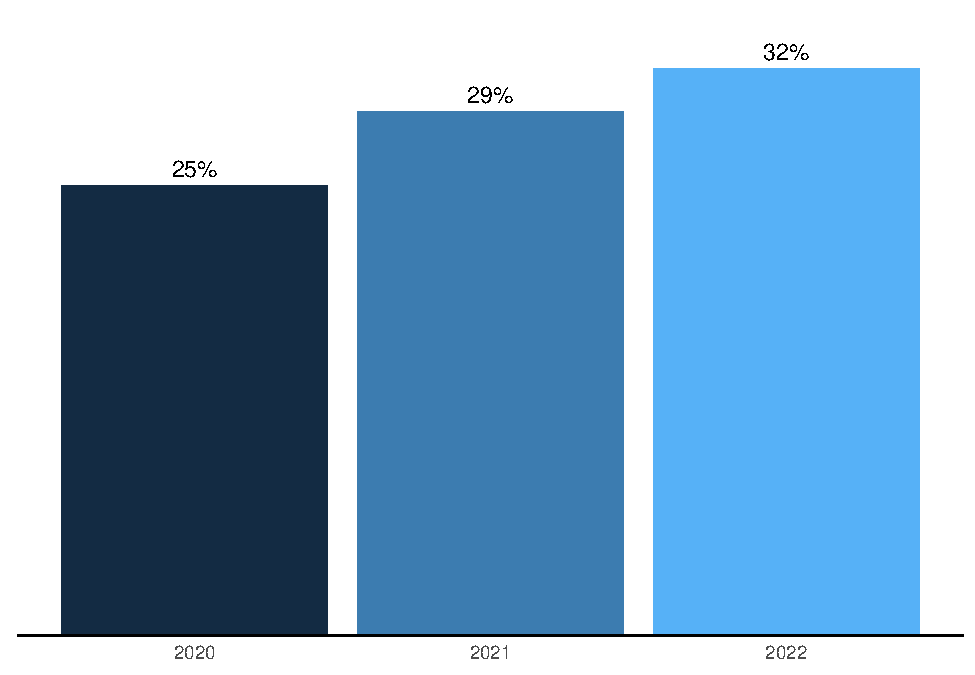
\includegraphics{Censo-SUAS-2022_files/figure-latex/coord_cadunico-1} \caption[Percentual de Postos do Cadastro Único que possuem coordenador - Brasil, 2020 - 2021 - 2022]{Percentual de Postos do Cadastro Único que possuem coordenador - Brasil, 2020 - 2021 - 2022}\label{fig:coord_cadunico}\floatfoot{Fonte: MDS, Censo SUAS}
\end{figure}

\hypertarget{considerauxe7uxf5es-finais-revisar}{%
\section{Considerações Finais
(revisar)}\label{considerauxe7uxf5es-finais-revisar}}

A Assistência Social é uma política de previsibilidade constitucional
reafirmadas por Lei, Normas, decretos, pactos. Assim, faz-se essencial
padrões de gestão e comandos únicos em todos os entes federados. Os
dados históricos sinalizam avanços e desafios para gestão do SUAS.

Os órgãos gestores da assistência social, tanto estaduais quanto
municipais, são estruturas fundamentais para a execução deste política.
O significado do direito caminham junto com o planejamento, ofertas
continuadas, padrões de respostas, comandos unicos etc.

Assim, para consolidação desta política que faz-se universal nos
territórios,é fundamental em todos entes federados estruturas
administrativas indicadas nos pactos, Lei compatível com LOAS, conforme
deliberação das conferencias nacionais, comando único do gestor da pasta
entre outros.

Os dados sinalizam avanços, a respeito das subdivisões administrativas
que apresentavam maior percentual de formalização nos órgãos gestores
estaduais em 88,5\% dos estados. As que apresentavam menores percentuais
de formalização nos órgãos gestores estaduais eram as de Regulação do
SUAS (38,5\%) e de Gestão do Trabalho (57,7\%). Nos municípios,
destaca-se forte presença de formalização das gestões do Cadastro Único
e Bolsa Família, bem como a proteção social básica, com respectivamente
80,68\% e 77,90\% respectivamente.

Os recursos recebidos via transação fundo-a-fundo, garantem maior
qualidade na distribuição, já que estes são fiscalizados pelos órgãos de
controle social e passam pelo crivo das Comissões Intergestores
Bipartite e Tripartite. Sobre o repasse, destacam-se o avanço ao longo
dos anos nesta forma repasse aliado ao cofinanciamento, sendo mais
presente o cofinancimento a Proteção Social Especial.

Destaca-se também um tópico novo e de importancia para gestão de
informação do SUAS. O cadatsro único é uma ferramenta que visa
potencializar as funções de proteção socia, vigilancia socioassitencial
e defesa de direitos, Para isso, os dados promovem acesso a serviços e
progrmas, identificação das fmaílias e leitura dos territórios, bem como
parcerias e ações intersetoriais.

\hypertarget{unidades-do-suas}{%
\chapter{Unidades do SUAS}\label{unidades-do-suas}}

Essa seção apresenta informações sobre as unidades físicas do SUAS e sua
evolução ao longo do tempo. Esse item contempla as seguintes
informações: a) quantidade de unidades administrativas da rede
socioassistencial, b) informações sobre acessibilidade, c) situação do
imovél, d) disponibilidade de equipamentos como computador com acesso a
internet.

\hypertarget{centros-de-referuxeancia-de-assistuxeancia-social-cras}{%
\section{Centros de Referência de Assistência Social
(CRAS)}\label{centros-de-referuxeancia-de-assistuxeancia-social-cras}}

Os Centros de Referência de Assistência Social (CRAS) são definidos pelo
artigo 6º-C da Lei Orgânica de Assistência Social (LOAS) como unidades
públicas municipais destinadas à prestação de serviços, programas de
projetos da proteção social básica às famílias, devendo se localizar em
áreas com maiores índices de vulnerabilidade e risco social.

No Censo SUAS de 2022 foram identificados 8.557 CRAS, em 5.535
municípios brasileiros, o que indica que há pelo menos um CRAS em 99,4\%
dos municípios brasileiros.

O quantitativo de CRAS dobrou entre 2007 e 2022, passando de 4.195
unidades para 8.557. O \cref{fig:quantitativo-CRAS} apresenta a evolução
do quantitativo de CRAS por grandes regiões de desenvolvimento.

\begin{figure}
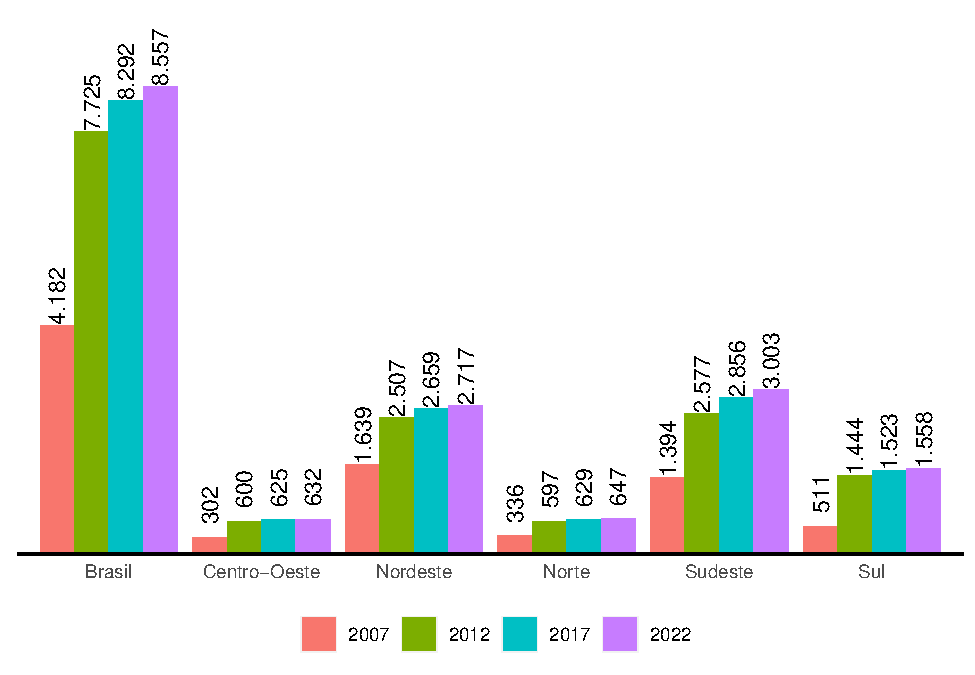
\includegraphics{Censo-SUAS-2022_files/figure-latex/quantitativo-CRAS-1} \caption[Evolução do quantitativo de CRAS, segundo grandes regiões]{Evolução do quantitativo de CRAS, segundo grandes regiões; 2007, 2012, 2017 e 2022}\label{fig:quantitativo-CRAS}\floatfoot{Fonte: MDS, Censo SUAS.}
\end{figure}

A Expansão em todo território nacional do número de CRAS evidencia a
consolidação de uma referencia de equipamento público de Assistêrncia
Social em todo território nacional. De acordo com os dados 99,37\%
municípios possuem CRAS, ou seja apenas 34 municípios no Brasil não
dispõe desta unidade
pública\footnote{estas informações são referentes ao preenchimento do Censo SUAS, é possível que no determinado período esta unidade pública não tenha preenchido o forumulário}.

Ao observar o número de CRAS por municípios, levando-se em conta o porte
populacional, verifica-se que os 35 municípios do país que não possuem
CRAS\footnote{é possível também que alguns deles não tenham respondido ao Censo SUAS}
e estão concentrados em municípios de pequeno porte
(\Cref{fig:CRAS-porte}).

Em relação a concentração de quantidade de CRAS, para os municípios de
pequeno porte I e pequeno porte II, dispõem, em sua maioria de uma
unidade de CRAS como referencia do território, sendo respectivamente
95,2\% e 71,5\%. Os municípios de médio porte, cerca de 67,3\% possuem
de 2 a 3 CRAS. Ja entre os municípios de grande porte, o grupo
majoritário de unidades são entre 4 a 6 CRAS - 52,5\%.

\begin{figure}
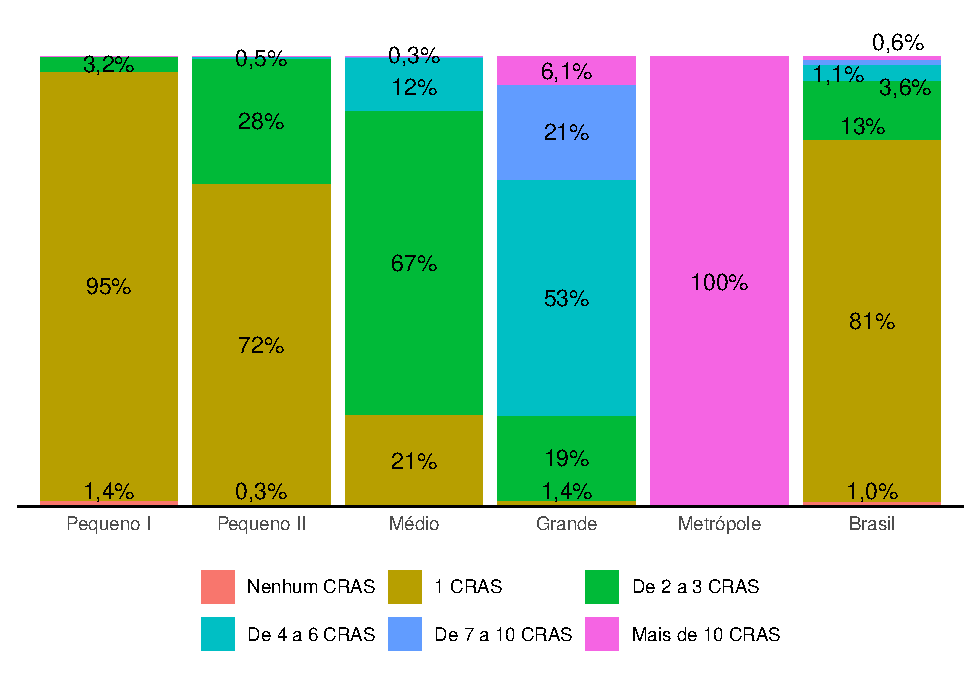
\includegraphics{Censo-SUAS-2022_files/figure-latex/CRAS-porte-1} \caption[Percentual de municípios por número de CRAS no município, segundo porte populacional estimado do município - Brasil, 2017]{Percentual de municípios por número de CRAS no município, segundo porte populacional estimado do município - Brasil, 2017}\label{fig:CRAS-porte}\floatfoot{Fonte: MDS, Censo SUAS; e IBGE, estimativas da população residente para os municípios}
\end{figure}

Os dados de CRAS que funcionam com imóvel próprio evoluiu
significativamente de 2008 a 2022. Destaca-se que o primeiro ano da
série histórica possuia 43,7\% CRAS com imóvel próprio
(\Cref{fig:CRAS-imovel}), dado que chega em 2022 com 59,62\%. Dados com
CRAS que funcionam com imóveis alugados passam por redução de 48,2\%
para 32,2\%.

Observa-se ainda aumento no percentual de CREAS que funcionam em imóveis
cedido: eram 6,8\% em 2008, o maior valor da série histórica chega a
9,1\% conforme o
\cref{fig:CRAS-imovel}\footnote{Para os anos de 2018 e 2019 esse dado não foi computado no Censo SUAS}.

\begin{figure}
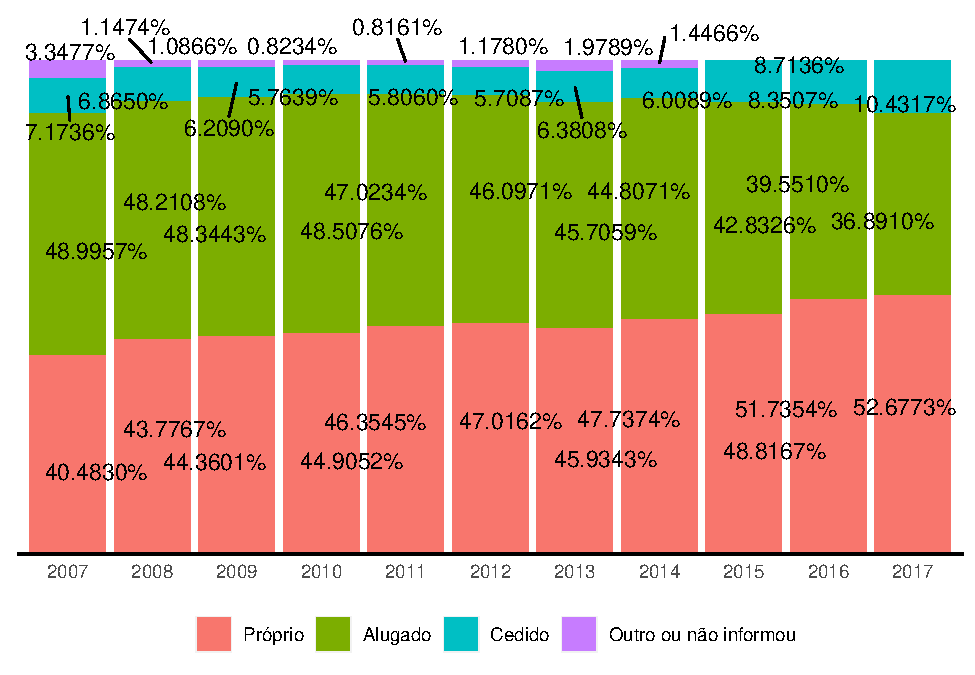
\includegraphics{Censo-SUAS-2022_files/figure-latex/CRAS-imovel-1} \caption[Evolução dos CRAS segundo situação do imóvel – Brasil, 2007 a 2022]{Evolução dos CRAS segundo situação do imóvel – Brasil, 2007 a 2022}\label{fig:CRAS-imovel}\floatfoot{Fonte: MDS, Censo SUAS.}
\end{figure}

A acessibilidade é importante para que os usuários da política consigam
chegar até os serviços oferecidos pelos CRAS. Em 2016, 38,7\% das
unidades declararam ter rota acessível ao banheiro de acordo com a Norma
da ABNT (NBR9050), enquanto que, em 37,8\% havia rota acessível aos
espaços do CRAS de acordo com a referida
Norma\footnote{foram considerados acesso adptado os imóveis que informam possui acessibildiade, de acordo com a norma ABNT ou não}.
Embora nenhuma das adaptações de acordo com a Norma da ABNT tenha estado
presente em mais de 40\% das unidades, todas as categorias relativas à
acessibilidade continuam crescendo percentualmente em relação aos anos
anteriores (\Cref{fig:CRAS-acessibilidade}).

\begin{figure}
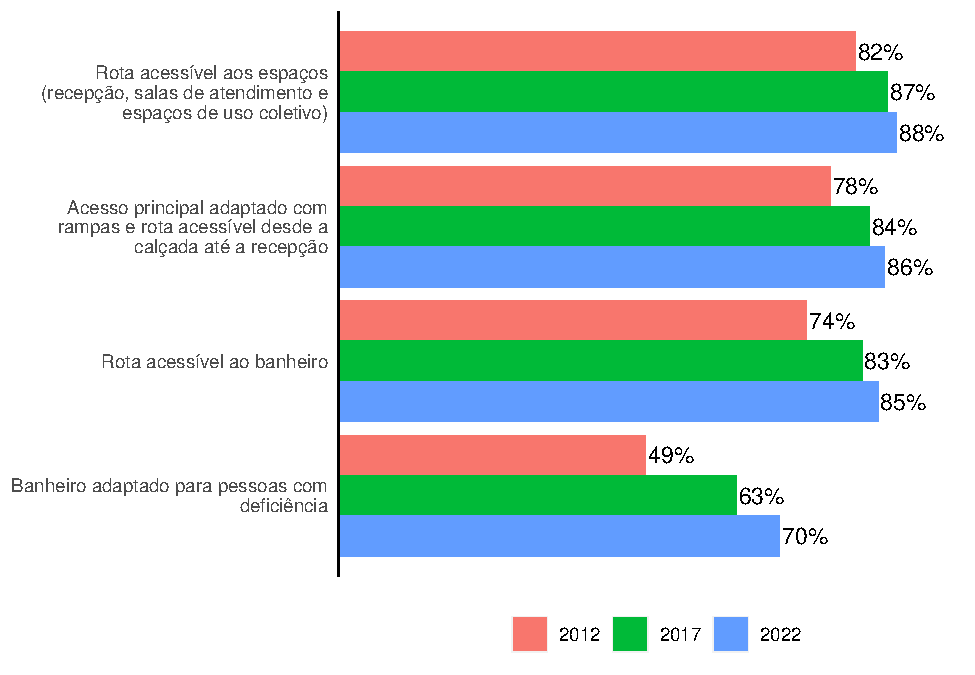
\includegraphics{Censo-SUAS-2022_files/figure-latex/CRAS-acessibilidade-1} \caption[Evolução percentual de CRAS com condições de acessibilidade - Brasil]{Evolução percentual de CRAS com condições de acessibilidade - Brasil; 2012, 2017 e 2022}\label{fig:CRAS-acessibilidade}\floatfoot{Fonte: MDS, Censo SUAS.}
\end{figure}

Os CRAS são considerados a porta de entrada da Assistência Social, sendo
uma referência para a população no território. Nesse sentido, podem se
articular com a rede de proteção social e com demais serviços ofertados
no município, de forma a garantir o acesso da população aos direitos
sociais.

Em 2016, verificou-se que as condições de acessibilidade em CRAS
localizados em imóveis próprios eram melhores que nas unidades situadas
em imóveis alugados ou cedidos. Entre os 4.263 CRAS que estavam
instalados em imóveis próprios, 51,9\% (2.212 unidades) possuíam
banheiro adaptado para pessoas com deficiência de acordo com a Norma
ABNT (NBR9050) e 53,2\% (2.267) rotas acessíveis ao banheiro. Dos 3.259
CRAS que funcionavam em imóveis alugados, 16,9\% (522 unidades) possuíam
banheiro adaptado para pessoas com deficiência e 21,3\% (694 unidades)
rota cessível ao banheiro. Entre os cedidos os percentuais eram 30,8 e
31,3, respectivamente, considerando o total de 718 Unidades
(\Cref{fig:CRAS-acessibilidade-situacao}).

Considerando a totalidade dos CRAS (8.240), 27,5\% dos CRAS que tinham
rota acessível ao banheiro de acordo com a Norma ABNT estavam instalados
em imóveis próprios, contra 8,4\% em imóveis alugados.

De todos os CRAS em imóveis próprios, apenas 3,0\% informaram não ter
nenhuma condição de acessibilidade, ainda que em desacordo com a norma
ABNT. Para os CRAS localizados em imóveis alugados esse percentual foi
de 11,6\% e em imóveis cedidos de 8,4\%.

\begin{figure}
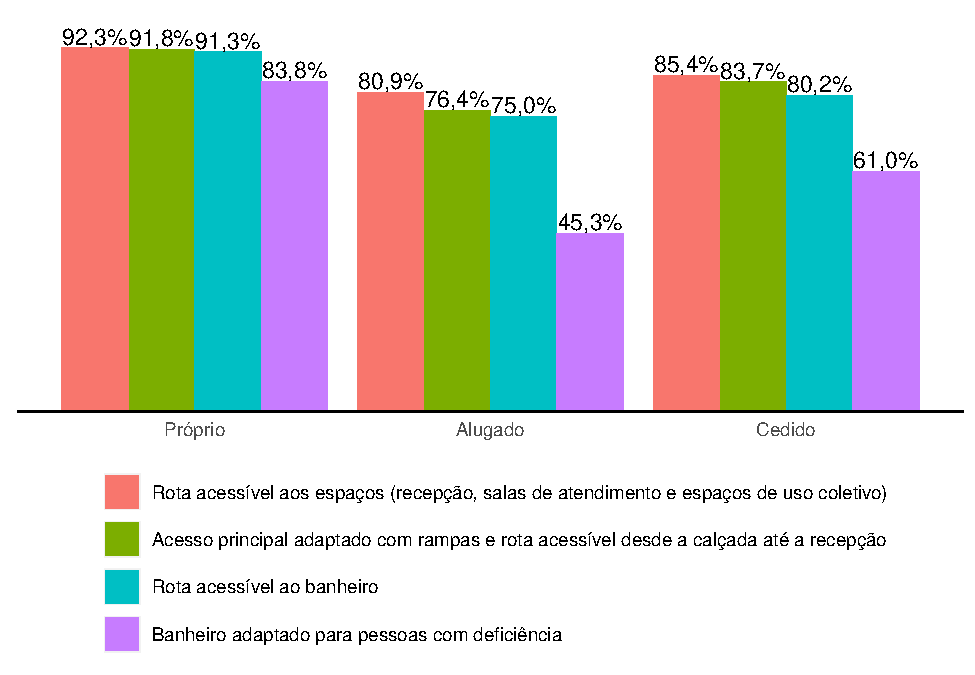
\includegraphics{Censo-SUAS-2022_files/figure-latex/CRAS-acessibilidade-situacao-1} \caption[Percentual de CRAS com condições de acessibilidade por situação do imóvel – Brasil, 2022]{Percentual de CRAS com condições de acessibilidade por situação do imóvel – Brasil, 2022}\label{fig:CRAS-acessibilidade-situacao}\floatfoot{Fonte: MDS, Censo SUAS.}
\end{figure}

O número absoluto e o percentual de CRAS com acesso à internet aumentam
desde 2007 chegando no último ano desta série com mais de 99\% das
unidades com computadores com acesso a internet conforme o
\cref{fig:CRAS-internet-percentual}.

\begin{figure}
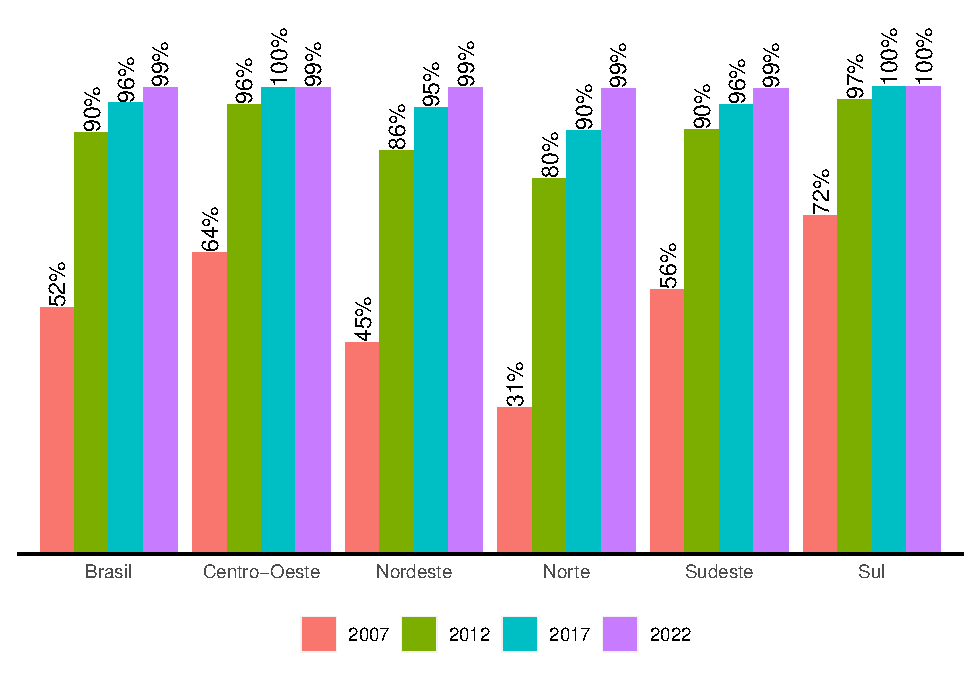
\includegraphics{Censo-SUAS-2022_files/figure-latex/CRAS-internet-percentual-1} \caption[Evolução percentual de CRAS com computadores com acesso à internet – Brasil]{Evolução percentual de CRAS com computadores com acesso à internet – Brasil; 2007, 2012, 2017 e 2022}\label{fig:CRAS-internet-percentual}\floatfoot{Fonte: MDS, Censo SUAS.}
\end{figure}

Em relação a CRAS com locais para Cadastro Único, o dado abaixo trás o
percentual destas informações e a disposição de equipes para esta
finalidade. Nota-se o aumento ao longo dos anos com CRAS que possuem
Cadastro Único com equipe exclusiva (\Cref{fig:equip-cadunico-cras}).

\begin{figure}
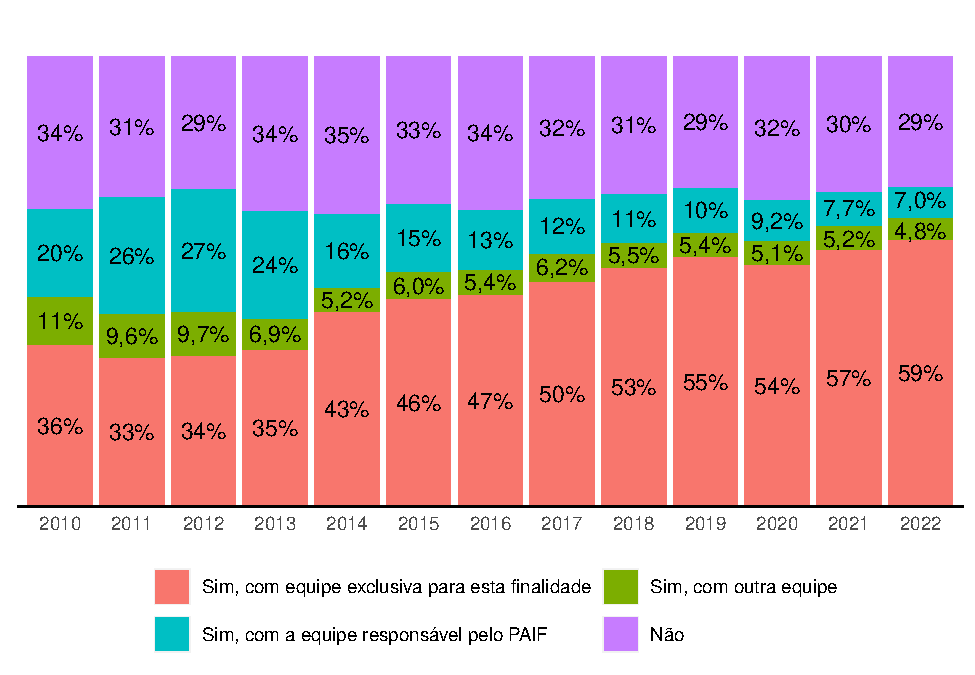
\includegraphics{Censo-SUAS-2022_files/figure-latex/equip-cadunico-cras-1} \caption[Percentual de CRAS com locais para CadÚnico - 2017 - 2022]{Percentual de CRAS com locais para CadÚnico - 2017 - 2022}\label{fig:equip-cadunico-cras}\floatfoot{Fonte: MDS, Censo SUAS}
\end{figure}

\hypertarget{centros-de-convivuxeancia}{%
\section{Centros de Convivência}\label{centros-de-convivuxeancia}}

Os Centros de Convivência, juntamente com os Centros de Referência de
Assistência Social (CRAS), são unidades que executam o Serviço de
Convivência e Fortalecimento de Vínculos e compõem a Rede de Proteção
Social Básica. Desde 2014 o número de Centros de Convivência no Brasil
aumentou, passando de 7.882 unidades em 2014 para 8.454 em 2016, em um
acréscimo de 572 unidades. A região Norte tem a menor quantidade de
unidades (238 ou 2,8\% do total), seguida do Centro-Oeste com 568
Unidades (ou 6,7\% do total). A região Sudeste tem o maior número de
Centros de Convivência, com 4.035 Unidades (47,7\% do total)

Os Centros de Convivência podem ser unidades públicas ou vinculadas a
entidades de assistência social, inscritas nos Conselhos de Assistência
Social do município ou do DF. Em 2016, 44,7\% dos Centros de Convivência
eram governamentais (total de 3.781 unidades) e 55,3\% das unidades eram
não governamentais (4.672 unidades). Desde 2014, o percentual de
unidades de natureza não governamental vem se reduzindo, passando de
57,4\% (4.521 unidades) para 55,3\% (4.672 unidades) em 2016 (Gráfico
29).

\begin{figure}
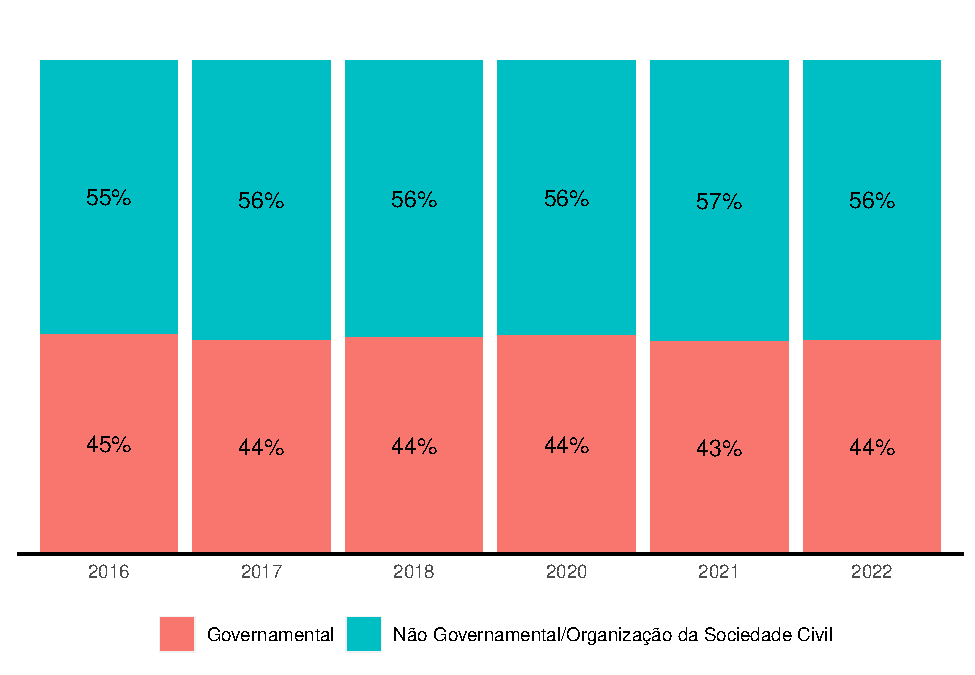
\includegraphics{Censo-SUAS-2022_files/figure-latex/centro-conv-natureza-1} \caption[Quantitativo de Centros de Convivência por Natureza da Unidade - BRASIL]{Quantitativo de Centros de Convivência por Natureza da Unidade - BRASIL; 2016 a 2022}\label{fig:centro-conv-natureza}\floatfoot{Fonte: MDS, Censo SUAS.}
\end{figure}

Em 2016, 31,2\% dos Centros de Convivência (2.636 unidades) possuíam
rota acessível ao banheiro de acordo com a norma da ABNT (NBR9050),
sendo a adaptação mais observada nas unidades. Todas as condições de
acessibilidade melhoraram em relação aos anos anteriores, e o maior
aumento foi verificado no percentual de Centros de Convivência com
banheiros adaptados para pessoas com deficiência: estavam presentes em
24,3\% das unidades em 2014 (1.918) e passaram a ser observados em
28,3\% das unidades em 2016 (2.389) (Gráfico 30).

\hypertarget{centro-de-referuxeancia-especializada-de-assistuxeancia-social-creas}{%
\section{Centro de Referência Especializada de Assistência Social --
CREAS}\label{centro-de-referuxeancia-especializada-de-assistuxeancia-social-creas}}

Os Centros de Referência Especializados de Assistência Social (CREAS)
são unidades públicas estatais que ofertam serviços da Proteção Social
Especial a pessoas e famílias em situação de risco pessoal ou social
e/ou em situação de violação de direitos.

O Censo SUAS 2022 registrou 2.846 CREAS no país: um incremento de 679
novas unidades em relação aos últimos 10 anos. O
\cref{fig:creas-quantitativo} sinaliza esta evolução por Regiões do
país.

\begin{figure}
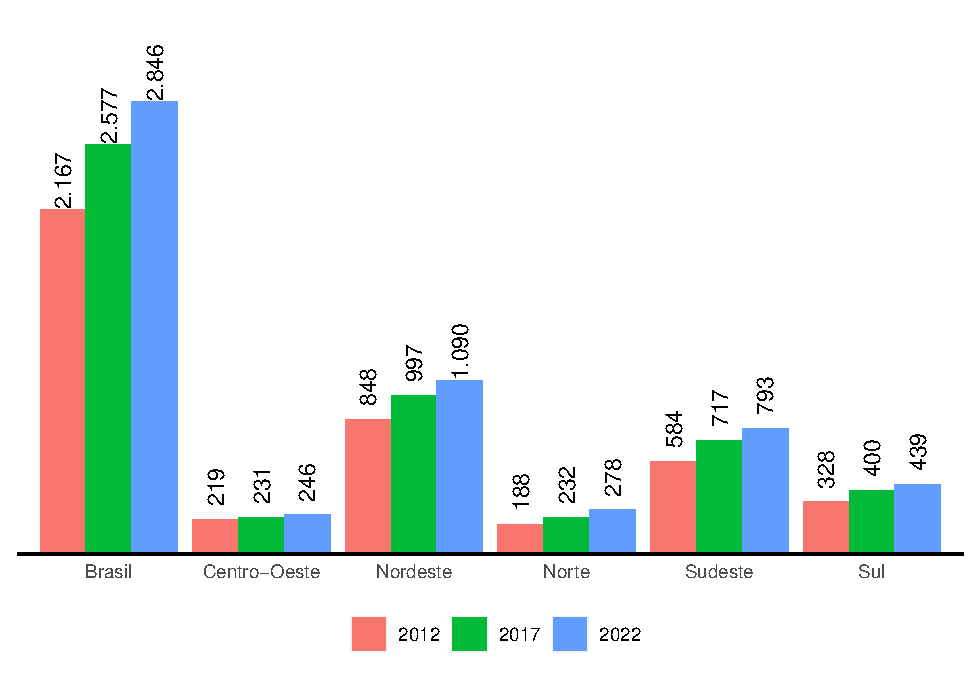
\includegraphics{Censo-SUAS-2022_files/figure-latex/creas-quantitativo-1} \caption[Evolução do quantitativo de CREAS, segundo grandes regiões]{Evolução do quantitativo de CREAS, segundo grandes regiões; 2012, 2017 e 2022}\label{fig:creas-quantitativo}\floatfoot{Fonte: MDS, Censo SUAS.}
\end{figure}

De acordo com os dados do \cref{fig:CREAS-porte} na qual sinaliza o
número de CREAS por município, levando-se em conta o porte populacional,
verifica-se que 54\% dos municípios não possuem CREAS. Eeles estão
concetrados nos municípios de Pequeno Porte I e II respectivamente com
77\% e 5,3\% dos municípios que não possuem esta unidade especializada.

\begin{figure}
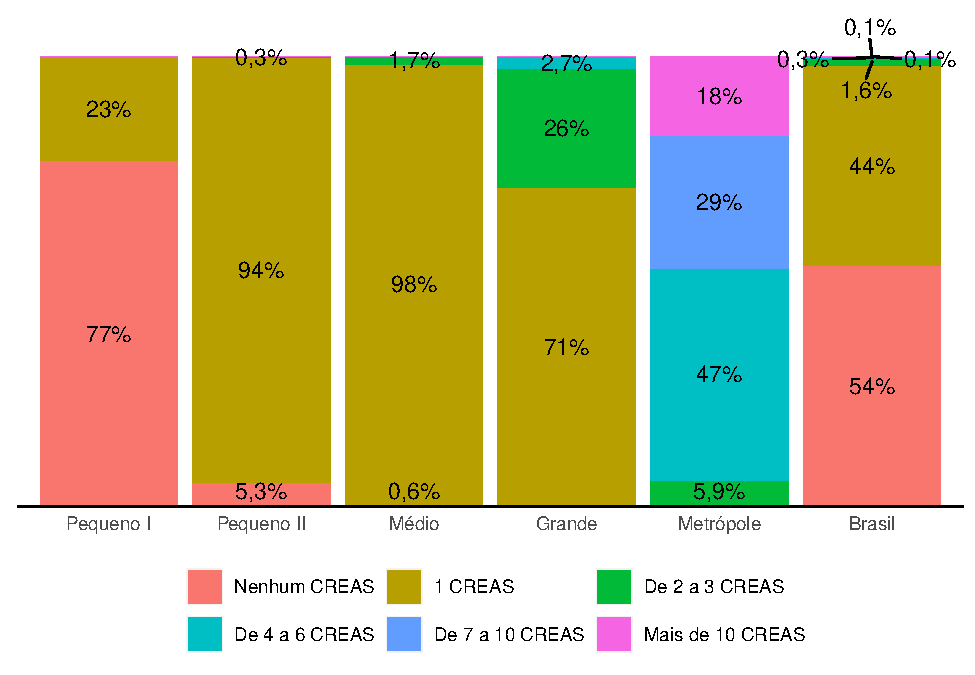
\includegraphics{Censo-SUAS-2022_files/figure-latex/CREAS-porte-1} \caption[Percentual de municípios por número de CREAS, segundo porte populacional - Brasil, 2022]{Percentual de municípios por número de CREAS, segundo porte populacional - Brasil, 2022}\label{fig:CREAS-porte}\floatfoot{Fonte: MDS, Censo SUAS; e IBGE, estimativas da população residente para os municípios}
\end{figure}

Ao observar a série histórica do \cref{fig:creas-situacao}, é possível
perceber que os imovéis próprios vem aumentando ao longo do tempo. Em
2012 eram 27\% das unidades e, chegam em 2022 com 37\%. Ao passo que os
imóveis próprios aumentam em 10\% pontos percentuais, os imovéis
alugados descrecem neste mesmo ponto computado no censo suas de 2022 com
57\% das undiades alugadas.Há também registros de imoveis cedidos na
qual ao longo dos anos sinalizam um leva
aumento\footnote{Para os anos de 2018 e 2019 esse dado não foi computado no Censo SUAS}.

\begin{figure}
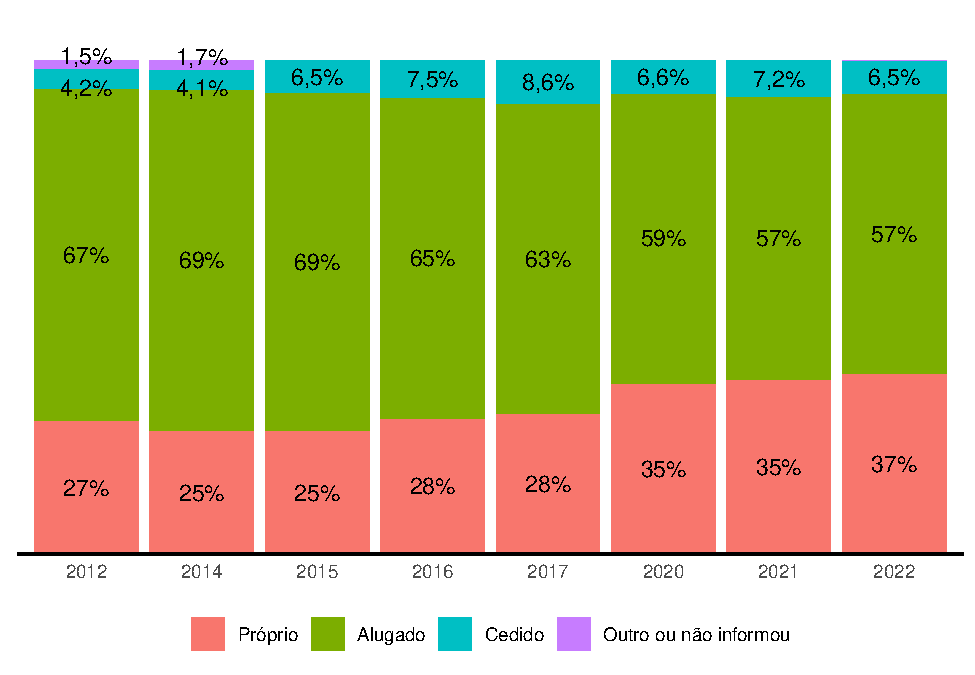
\includegraphics{Censo-SUAS-2022_files/figure-latex/creas-situacao-1} \caption[Evolução dos CREAS segundo situação do imóvel – Brasil]{Evolução dos CREAS segundo situação do imóvel – Brasil; 2012, 2017 e 2022}\label{fig:creas-situacao}\floatfoot{Fonte: MDS, Censo SUAS.}
\end{figure}

De acordo com os dados do Censo SUAS de 2012, 33\% dos CREAS possuíam
banheiro adaptado para pessoas com mobilidade reduzida. Em 2022 há um
crescimento de 22 pontos percentuais em relação ao ano de 2012, com 55\%
dos CREAS com essa estrutura
adptada\footnote{foram considerados acesso adptado os imóveis que informam possui acessibildiade, de acordo com a norma ABNT ou não}.

A presença de acesso principal adaptado com rota ascessível aos espaços
(recepção, salas de atendimento e espaços de uso coletivo) é a mais
presente nas unidades de CREAS com destaque para 83\% no CENSO SUAS de
2022.

O \cref{fig:creas-acessibilidade} referencia outras adpções como com
rampas, rota acessível e calçada e de rota acessível ao banheiro. todas
essas adaquações amliaram a acessibildiade ao longo dos anos.

\begin{figure}
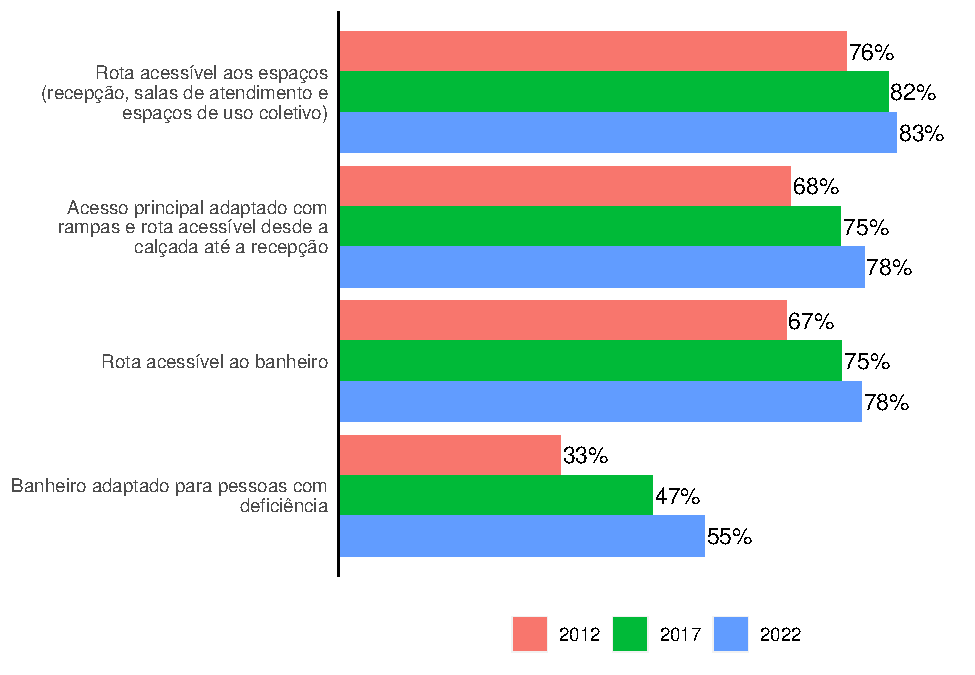
\includegraphics{Censo-SUAS-2022_files/figure-latex/creas-acessibilidade-1} \caption[Evolução percentual de CREAS com condições de acessibilidade - Brasil]{Evolução percentual de CREAS com condições de acessibilidade - Brasil; 2012, 2017 e 2022}\label{fig:creas-acessibilidade}\floatfoot{Fonte: MDS, Censo SUAS.}
\end{figure}

O \cref{fig:CREAS-acessibilidade-situacao} através do Censo SUAS 2022
apurou a situação do imóvel com a presença das condições de
acessibilidade. Os dados sinalizam que a acessibilidade é mais presente
em imovéis próprios.

\begin{figure}
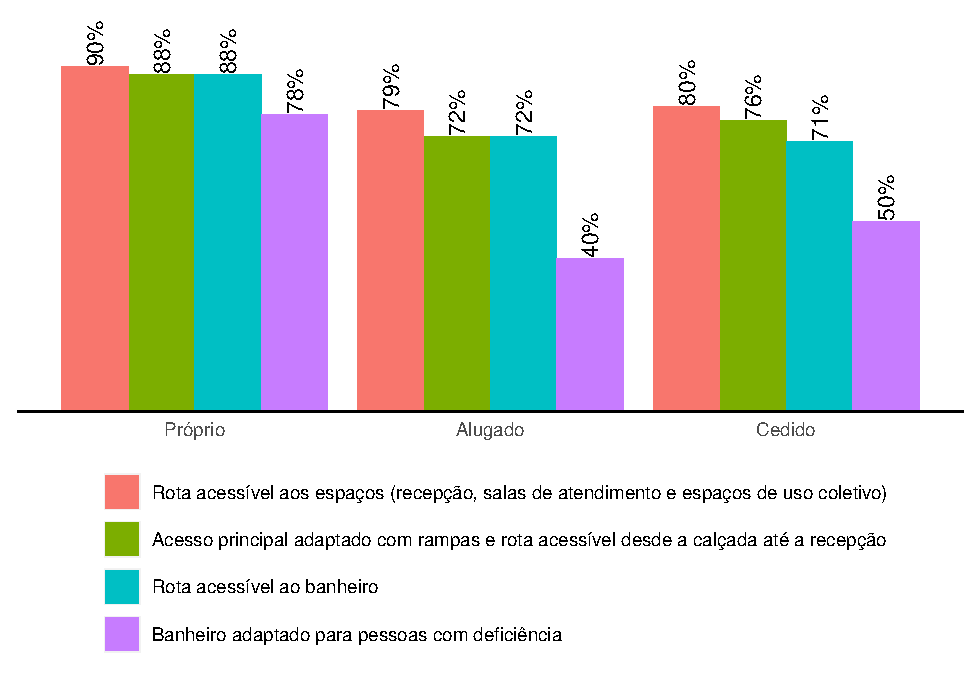
\includegraphics{Censo-SUAS-2022_files/figure-latex/CREAS-acessibilidade-situacao-1} \caption[Evolução percentual de CREAS com condições de acessibilidade por situação do imóvel – Brasil, 2022]{Evolução percentual de CREAS com condições de acessibilidade por situação do imóvel – Brasil, 2022}\label{fig:CREAS-acessibilidade-situacao}\floatfoot{Fonte: MDS, Censo SUAS.}
\end{figure}

A existência de computadores com acesso à internet é um importante
aspecto a ser observado quando se avalia a infraestrutura dos CREAS. Em
2022, 99\% dos CREAS possuem computadores com acesso à internet conforme
o \cref{fig:CREAS-internet-percentual}. Números que avançou em todas as
regiões, em especial, na Região Norte conforme linha histórica desta
evolução apresentada no gráfico abaixo.

\begin{figure}
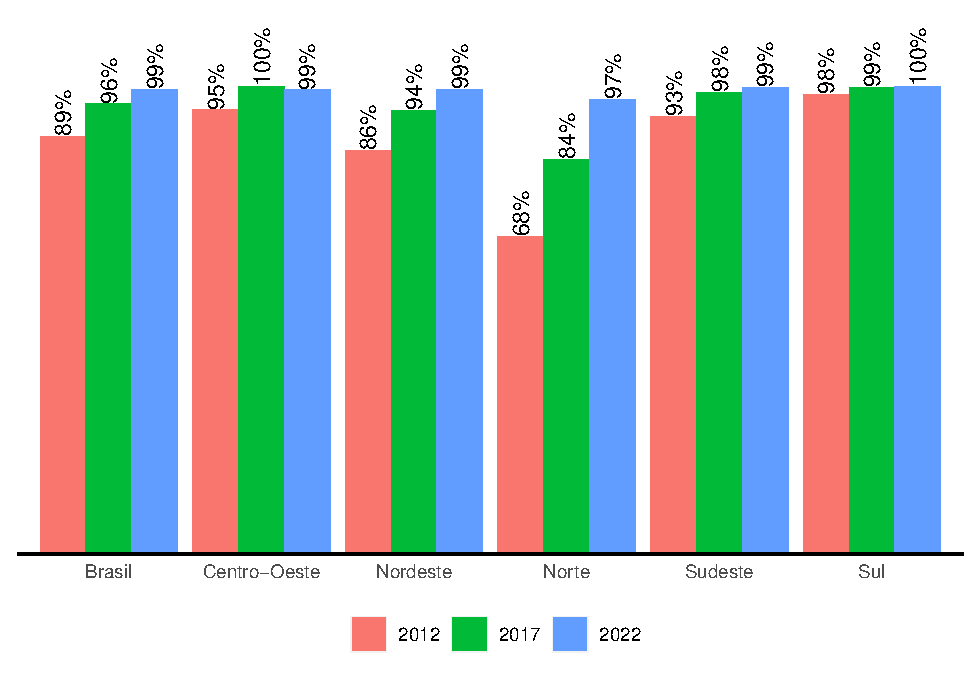
\includegraphics{Censo-SUAS-2022_files/figure-latex/CREAS-internet-percentual-1} \caption[Evolução percentual de CREAS com computadores com acesso à internet – Brasil]{Evolução percentual de CREAS com computadores com acesso à internet – Brasil; 2012, 2017 e 2022}\label{fig:CREAS-internet-percentual}\floatfoot{Fonte: MDS, Censo SUAS.}
\end{figure}

\begin{figure}
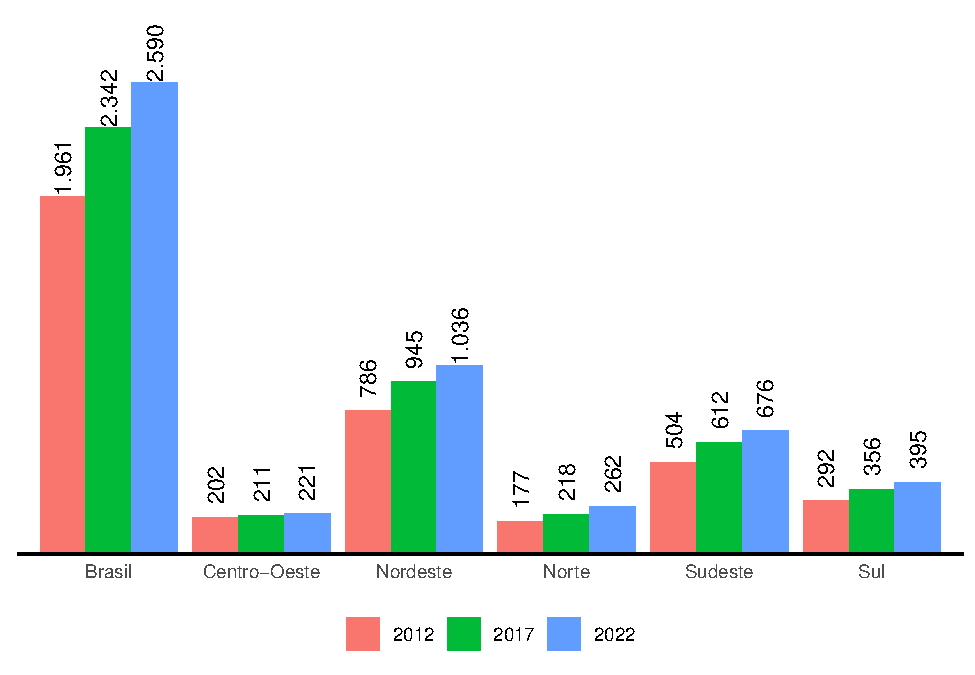
\includegraphics{Censo-SUAS-2022_files/figure-latex/CREAS-quantidade-municipios-1} \caption[Evolução do quantitativo de municípios com CREAS, Brasil e grandes regiões - 2012, 2017 e 2022]{Evolução do quantitativo de municípios com CREAS, Brasil e grandes regiões - 2012, 2017 e 2022}\label{fig:CREAS-quantidade-municipios}\floatfoot{Fonte: MDS, Censo SUAS}
\end{figure}

A oferta regionalizada de CREAS é uma estratégia que objetiva garantir a
universalização do acesso e integralidade do antendimento da proteção
socioassistencia especializada. Estar prevista através da Resolução
31/2013 do CNAS. Essa composição é organziada através dos entes
estaduais e o \cref{fig:creas-regionais} sinaliza a evolução dessa
oferta.

\begin{figure}
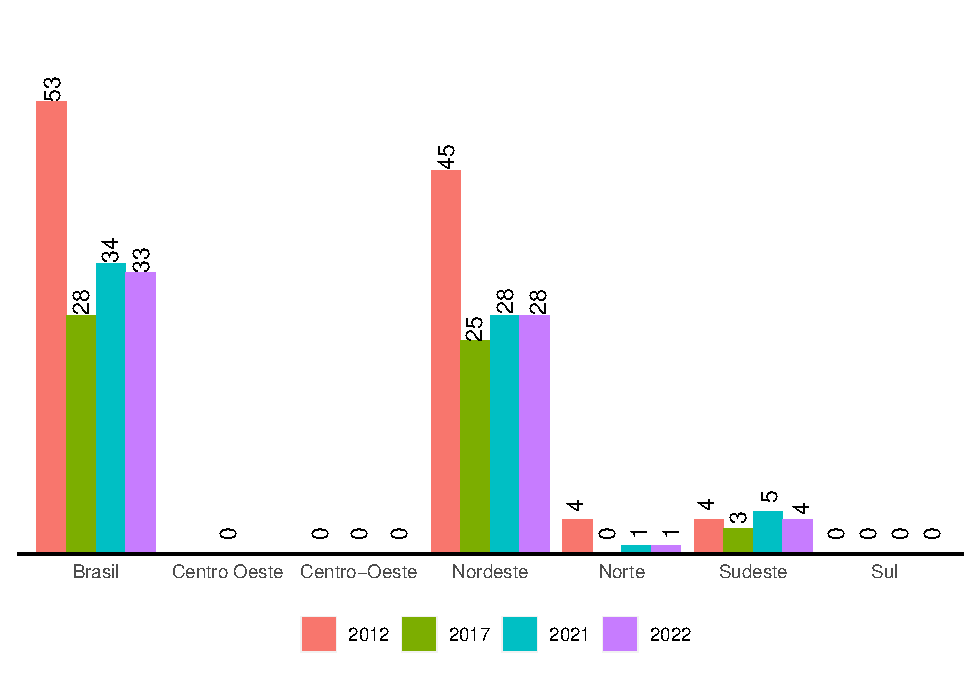
\includegraphics{Censo-SUAS-2022_files/figure-latex/creas-regionais-1} \caption[Evolução do quantitativo de CREAS Regionais, Brasil e grandes regiões - 2012, 2017 e 2022]{Evolução do quantitativo de CREAS Regionais, Brasil e grandes regiões - 2012, 2017 e 2022}\label{fig:creas-regionais}\floatfoot{Fonte: MDS, Censo SUAS.}
\end{figure}

\hypertarget{centro-de-referuxeancia-especializado-para-populauxe7uxe3o-em-situauxe7uxe3o-de-rua-centro-pop}{%
\section{Centro de Referência Especializado para População em Situação
de Rua -- Centro
POP}\label{centro-de-referuxeancia-especializado-para-populauxe7uxe3o-em-situauxe7uxe3o-de-rua-centro-pop}}

Os Centros de Referência Especializados para População em Situação de
Rua (Centros POP) são unidades públicas que oferecem atendimento
especializado para a população em situação de rua, no âmbito da proteção
social especial de média complexidade.

Entre 2012 e 2022 o número de Centros POP cresceu, passando de 105
unidades para 237 no período. O \cref{fig:quantitativo-CentroPop}
sinaliza a essa evolução na escala de a cada 5 anos por Regiões do
Brasil.

\begin{figure}
\includegraphics{Censo-SUAS-2022_files/figure-latex/quantitativo-CentroPop-1} \caption[Evolução do quantitativo de Centro Pop, 2012 a 2022]{Evolução do quantitativo de Centro Pop, 2012 a 2022}\label{fig:quantitativo-CentroPop}\floatfoot{Fonte: MDS, Censo SUAS}
\end{figure}

Os Centro Pop estão presentes em municípios de grande porte e
metrópoles, o \cref{fig:cpop-porte} sinaliza que 59\% dos municípios de
grande porte possui pelo menos uma unidade, e para metropoles 100\%
possuem unidades de centro pop, sendo 59\% entre duas a três unidades,
24\% uma unidade e 18\% de 4 a 6 undiades de Centro Pop. Há presenta
também em múnicípios de médio porte, com destaque para 5,9\% dos
municípios.

\begin{figure}
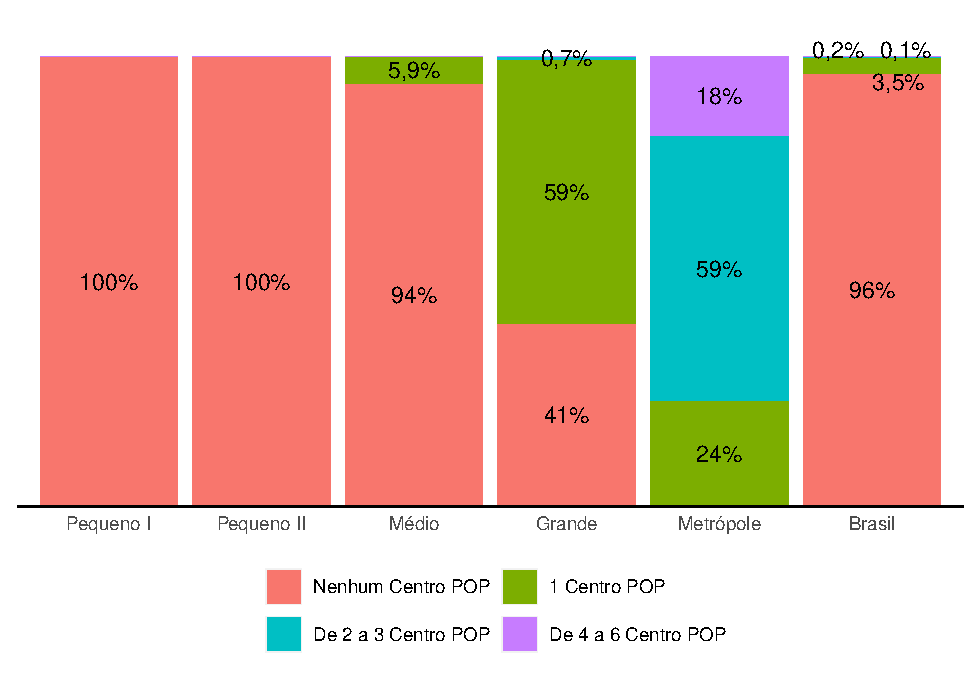
\includegraphics{Censo-SUAS-2022_files/figure-latex/cpop-porte-1} \caption[Percentual de municípios por número de Centro POP, segundo porte populacional - Brasil, 2022]{Percentual de municípios por número de Centro POP, segundo porte populacional - Brasil, 2022}\label{fig:cpop-porte}\floatfoot{Fonte: MDS, Censo SUAS; e IBGE, estimativas da população residente para os municípios}
\end{figure}

Em relação a acessibilidade dos Centro Pop o
\cref{fig:cpop-acessibilidade-situacao} relaciona esta adaptação com a
situação do imóvel. No geral todoas as adaptações de acessibildiade são
superiores ao serem relacionadas com os imóveis alugados. Em relação aos
imóveis cedidos, a adaptação de banheiro se sobressai em relação as
demais situações dos imóveis.

\begin{figure}
\includegraphics{Censo-SUAS-2022_files/figure-latex/cpop-acessibilidade-situacao-1} \caption[Percentual de Centros POP com condições de acessibilidade segundo situação do imóvel – Brasil, 2022]{Percentual de Centros POP com condições de acessibilidade segundo situação do imóvel – Brasil, 2022}\label{fig:cpop-acessibilidade-situacao}\floatfoot{Fonte: MDS, Censo SUAS.}
\end{figure}

Em 2016,95\% dos Centros Pop destacam computador com acesso à internet
em 2022. O \cref{fig:cpop-internet-percentual} referencia essa evolução
por Regiões do Brasil, as regiões Centro Oeste e Sul possuem 100\% das
undiades com acesso a internet e a região Norte com maior desafio de
acesso, com 75\% das unidades de Centro Pop com acesso a internet.

\begin{figure}
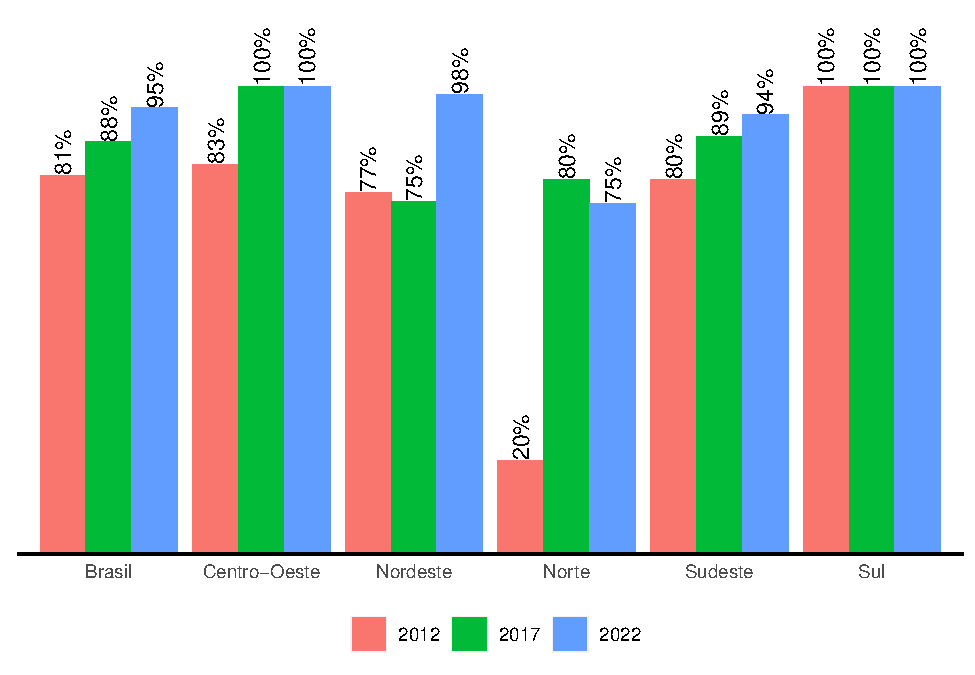
\includegraphics{Censo-SUAS-2022_files/figure-latex/cpop-internet-percentual-1} \caption[Percentual de Computadores nos Centro Pop com acesso a internet, 2012 a 2022]{Percentual de Computadores nos Centro Pop com acesso a internet, 2012 a 2022}\label{fig:cpop-internet-percentual}\floatfoot{Fonte: MDS, Censo SUAS.}
\end{figure}

\hypertarget{centro-dia}{%
\section{Centro-Dia}\label{centro-dia}}

Centro Dia são unidades públicas especializadas para qtender pessoas com
deficiência e suas famílias. Ela estar inserida no ambito da proteção
social espceial de média complexidade. No ano de 2015 identifica-se no
Brasil 1.340 unidades. Em 2022 há um crescimento de 40,7\% destas
unidades conforme pode ser observada no
\cref{fig:quantitativo-Centrodia}.

\begin{figure}
\includegraphics{Censo-SUAS-2022_files/figure-latex/quantitativo-Centrodia-1} \caption[Evolução do quantitativo de Centro dia, segundo grandes regiões]{Evolução do quantitativo de Centro dia, segundo grandes regiões; 2015 a 2022}\label{fig:quantitativo-Centrodia}\floatfoot{Fonte: MDS, Censo SUAS.}
\end{figure}

Em relação a natureza destas unidades, o \cref{fig:cdia-natureza}
sinaliza a frequencia histórica de unidades referenciadas pelas
Organizações da Sociedade Civil (OSCs). Das undiades destacadas no Censo
SUAS 2022, 92,8\% são ofertadas por OSCs.

\begin{figure}
\includegraphics{Censo-SUAS-2022_files/figure-latex/cdia-natureza-1} \caption[Quantitativo de Centros Dia por Natureza da Unidade - BRASIL, 2015 a 2022]{Quantitativo de Centros Dia por Natureza da Unidade - BRASIL, 2015 a 2022}\label{fig:cdia-natureza}\floatfoot{Fonte: MDS, Censo SUAS.}
\end{figure}

Em relação a acessibilidade destas unidades, o banheiro acessivel é a
adaptação mais presentes nestas unidades chegando nos registros do Censo
SUAS de 2022 com 73\%. Como trata-se de unidades especializadas para
atenção a pessoas com deficiência, esse item é de funmental importância
para assegurar acolhida e segurança a este público e suas famílias. O
\cref{fig:cdia-acessibilidade} sinaliza os locais e composição de
acessibilidade, estes dados sinalizam um desafio para garantir as
condições físicas de acesso ao público de pessoas com deficiência nas
undiades de Centro Dia.

\begin{figure}
\includegraphics{Censo-SUAS-2022_files/figure-latex/cdia-acessibilidade-1} \caption[Evolução percentual de Centro Dia com condições de acessibilidade - Brasil]{Evolução percentual de Centro Dia com condições de acessibilidade - Brasil; 2015, 2018 e 2022}\label{fig:cdia-acessibilidade}\floatfoot{Fonte: MDS, Censo SUAS.}
\end{figure}

Além disto, há outras adaptações importantes netsas undiades, coo
tecnologias assistidas, suportes com materiais em Braile, profissionais
com conhecimento em Libras entre outros destacados no grafico abaixo:

\begin{figure}
\includegraphics{Censo-SUAS-2022_files/figure-latex/cdia_adaptações-1} \caption[Quantidade de Centro Dia, segundo outras adaptações - Brasil, 2015, 2018 e 2022]{Quantidade de Centro Dia, segundo outras adaptações - Brasil, 2015, 2018 e 2022}\label{fig:cdia_adaptações}\floatfoot{Fonte: MDS, Censo SUAS.}
\end{figure}

\hypertarget{unidades-de-alta-complexidade}{%
\section{Unidades de Alta
Complexidade}\label{unidades-de-alta-complexidade}}

As Unidades de Acolhimento tem o objetivo de ofertar serviços de
Proteção Social Especial de Alta Complexidade, com atenção a pessoas
e/ou famílias com vínculos rompidos ou fragilizados, ou que estejam em
situação de abandono, ameaça ou violação de direitos, de forma a
garantir sua proteção integral.

As informações sobre as Unidades de Acolhimento que são tipificadas,
sinalizam um crescimento em todos os
públicos.\footnote{Resolução CNAS 109/2009}. Através do
\cref{fig:unac-publico} destaca-se as seguintes informações sobre as
Unidades de Acolhimento Institucional:

\begin{itemize}
\item
  Crianças e Adolescentes: há 2.916 Unidades, no período entre 2014 e
  2022 houve um crescimento de 6\% no Brasil;
\item
  Pessoas Iodsas: há 2.059 Unidades, no período entre 2014 e 2022 houve
  um crescimento de 42\% no Brasil;
\item
  Adultos e Famílias: há 997 Unidades, no período entre 2014 e 2022
  houve um crescimento de 64\% no Brasil;
\item
  Exclusivamente Pessoas Adultas com Deficiência: há 362 Unidades, no
  período entre 2014 e 2022 houve um crescimento de 83\% no
  Brasil\footnote{As unidades de Residência Inclusiva são as unidades tipificadas para atendimento de jovens e adultos com deficiência. Assim, entende-se a característica do público de unidades exclusivas para pessoas Adultas com Deficiência deve estar alinhado esta caracterisica de unidade de acolhimento}.
\item
  Mulheres em Situação de Violência Doméstica ou Familiar: há 112
  Unidades, no período entre 2014 e 2022 houve um crescimento de 14\% no
  Brasil;
\item
  Jovens Egressos dos Serviços de Acolhimento: há 67 Unidades, no
  período entre 2014 e 2022 houve um crescimento de 72\% no
  Brasil\footnote{O Serviços de República é a descrição tipificada para prioritariamente público de 18 a 21 anos após desligamento de serviços de acolhimento insitucional}.
\end{itemize}

No que se refere a unidades de atenção exclusiva para crianças com
deficiência não é uma unidade tipificada, sendo a orientação deste
público estar em unidades de acolhimento para Crianças e Adolescentes.
Como destaca o \cref{fig:unac-publico} trata-se de uma unidade que vem
reduzindo ao longo do tempo.

\begin{figure}
\includegraphics{Censo-SUAS-2022_files/figure-latex/unac-publico-1} \caption[Quantidade de Unidades de Acolhimento por principal público atendido  - 2014 - 2022]{Quantidade de Unidades de Acolhimento por principal público atendido  - 2014 - 2022}\label{fig:unac-publico}\floatfoot{Fonte: MDS, Censo SUAS.}
\end{figure}

No que se refere a quantidade total destas unidades de acolhimento por
porte populacional, destaca-se que há concentração nos municípios de
grande porte e metrópole. Todas as metrópoles possuem registro de mais
de 10 unidades. O \cref{fig:unac-porte} também sinaliza que 74\% dos
municípios de pequeno porte I não dispõem de serviços de alta
complexidade.

Para os municípios menores a Resolução 31/2013 do CNAS sinaliza sobre a
oferta regionalizada sobre a expansão qualificada dos serviços de Alta
Complexidade para Criança e Adolescentes. Para esses municípios, faz-se
importante diagnóstico para analise de oferta regionalizada desta
unidade de Alta Complexidade.

\begin{figure}
\includegraphics{Censo-SUAS-2022_files/figure-latex/unac-porte-1} \caption[Quantidade de Unidades de Acolhimento, segundo porte populacional - Brasil, 2022]{Quantidade de Unidades de Acolhimento, segundo porte populacional - Brasil, 2022}\label{fig:unac-porte}\floatfoot{Fonte: MDS, Censo SUAS; e IBGE, estimativas da população residente para os municípios}
\end{figure}

A maioria das Unidades de Acolhimento são executadas por Organizações da
Sociedade Cívil (Osc). Esse percentual teve uma redução entre 2012 e
2022. Em 2012 estes dados sinalizam percentual de 66,4\% das unidades de
acolhimento com execução de OSC, registrando em 2022 63,4\% conforme o
\cref{fig:acolh_nat}

\begin{figure}
\includegraphics{Censo-SUAS-2022_files/figure-latex/acolh_nat-1} \caption[Quantitativo de Acolhimento Institucional por Natureza da Unidade - BRASIL, 2012 a 2022]{Quantitativo de Acolhimento Institucional por Natureza da Unidade - BRASIL, 2012 a 2022}\label{fig:acolh_nat}\floatfoot{Fonte: MDS, Censo SUAS.}
\end{figure}

No que se refere às condições de acessibilidade, é possível notar
melhorias no percentual dos quatro quesitos de acessibilidade. A
adaptação mais observada é a rota acessível ao banheiro, presente em
50,9\% das Unidades, e a menos observada é o acesso principal adaptado
com rampas e rota acessível desde a calçada até o interior da unidade,
presentes em 49,2\% das Unidades. O banheiro adaptado para pessoas com
deficiência e/ou mobilidade reduzida, presente em 47,9\% das unidades em
2022 e no que se refere ao acesso principal adaptado com rampas e e rota
acessivel para o censo suas 2022 observa-se presente em 45,6\% das
unidades conforme o \cref{fig:unac_acessibilidade}.

\begin{figure}
\includegraphics{Censo-SUAS-2022_files/figure-latex/unac_acessibilidade-1} \caption[Evolução percentual de Unidades de Acolhimento Municipais com condições de acessibilidade - Brasil]{Evolução percentual de Unidades de Acolhimento Municipais com condições de acessibilidade - Brasil; 2017 e 2022}\label{fig:unac_acessibilidade}\floatfoot{Fonte: MDS, Censo SUAS}
\end{figure}

Em relação ao acesso a internet, observa-se uma evolução nos últimos 10
anos. Em 2012 62,2\% das unidades possuem acesso a internet, o censo
suas de 2022 destaca que 100\% dos computadores das undiades possuem
acesso a internet conforme o \cref{fig:unac-internet}.

\begin{figure}
\includegraphics{Censo-SUAS-2022_files/figure-latex/unac-internet-1} \caption[Percentual de Computadores nas unidades de Acolhimento com acesso a internet, 2012, 2017 e 2022]{Percentual de Computadores nas unidades de Acolhimento com acesso a internet, 2012, 2017 e 2022}\label{fig:unac-internet}\floatfoot{Fonte: MDS, Censo SUAS.}
\end{figure}

\hypertarget{cadastro-uxfanico}{%
\section{Cadastro Único}\label{cadastro-uxfanico}}

Quanto a presença das unidades do Cadastro Único, os dados do Censo SUAS
2022 indicam a existência de 2.892 Postos do Cadastro Único. Número que
vem crescendo numa média Nacional de 14\% nos últimos 2 anos. Destaca-se
a Região do Centro Oeste na qual teve crescimento de 25\% neste mesmo
período.

Em relação ao local onde estão estas unidades,
\Cref{fig:posto_cadunico}. A maioria destas unidades, 60,9\% encontra-se
na secretaria de assistencia social. A segunda proporção são postos
exclusivos, com detaque para algumas undiades presentes em escolas,
conselhos e OSCS.

\begin{figure}
\includegraphics{Censo-SUAS-2022_files/figure-latex/posto_cadunico-1} \caption[Distribuição dos Postos do Cadastro Único - Brasil, 2020 a 2022]{Distribuição dos Postos do Cadastro Único - Brasil, 2020 a 2022}\label{fig:posto_cadunico}\floatfoot{Fonte: MDS, Censo SUAS.}
\end{figure}

A acessibilidade possui um leve avanço nos últimos anos, com execeção da
rota ascessivel aos principais espaços os demais itens de acessbilidade
avançaram conforme pode ser observado através do
\cref{fig:postcad-acessibilidade}.

\begin{figure}
\includegraphics{Censo-SUAS-2022_files/figure-latex/postcad-acessibilidade-1} \caption[Evolução percentual de postos do Cadastro Único com condições de acessibilidade - Brasil]{Evolução percentual de postos do Cadastro Único com condições de acessibilidade - Brasil; 2020, 2021 e 2022}\label{fig:postcad-acessibilidade}\floatfoot{Fonte: MDS, Censo SUAS.}
\end{figure}

Em relação aos espaços de acessibilidade comparada a situação do imóvel,
destaca-se que os postos do Cadastro Único próprios ou cedidos, possuem
significativamente mais ascessibilidade que os imóveis alugados
(\Cref{fig:postcad-acessibilidade-situacao}).

\begin{figure}
\includegraphics{Censo-SUAS-2022_files/figure-latex/postcad-acessibilidade-situacao-1} \caption[Percentual de Postos do Cadastro Único com condições de acessibilidade segundo situação do imóvel – Brasil, 2022]{Percentual de Postos do Cadastro Único com condições de acessibilidade segundo situação do imóvel – Brasil, 2022}\label{fig:postcad-acessibilidade-situacao}\floatfoot{Fonte: MDS, Censo SUAS.}
\end{figure}

Em relação a computadores com acesso a internet, os dados do censo suas
2022 sinaliza que 99\% das unidades dispõe de equipamentos com esta
estrutura conforme pode ser observado no
\cref{fig:postcad-internet-percentual}.

\begin{figure}
\includegraphics{Censo-SUAS-2022_files/figure-latex/postcad-internet-percentual-1} \caption[Evolução percentual de Postos do Cadastro Único com computadores com acesso à internet – Brasil]{Evolução percentual de Postos do Cadastro Único com computadores com acesso à internet – Brasil;  2020, 2021 e 2022}\label{fig:postcad-internet-percentual}\floatfoot{Fonte: MDS, Censo SUAS.}
\end{figure}

Os Serviços do SUAS são oferta continuadas \ldots{}

Busca garantir acesso a direitos sociais a quem necessitam. A
centralidade na família é \Cref{fig:quantitativo-CRAS}

\#Considerações Finais

Esta versão do Censo SUAS 2022 analisou xx unidades da Assistência
Social. Observa-se que no ambito a Proteção Básica existiu um
crescimento de 11\% nos últimos 10 anos. Acessibilidade: melhora
sobretudo os que possuem imóvel próprio que chegam a ter 28 pontos
percentuais de diferença em relação aos imóveis alugados.

No que se refere ao CREAS, observa-se um crescimento de 31\% destas
unidades nos últimos 10 anos. As condições de Acessibilidade dos CREAS
também evoluem, sobretudo os que possuem imóvel próprio com 28,4\% de
diferença em relação aos imovéis alugados.

Os Centro Pop crescem 126\% ao longo dos últimos 10 anos (confirmar)

Em relação as Unidades de Acolhimento Institucional 45\% delas são da
modalidade de Criança e Adolescente, em seguida para públicos de pessoas
Idosas e Adultos e Famílias.

\hypertarget{serviuxe7os-e-benefuxedcios-ofertados-pelo-suas}{%
\chapter{Serviços e Benefícios ofertados pelo
SUAS}\label{serviuxe7os-e-benefuxedcios-ofertados-pelo-suas}}

A Proteção remonta um conjunto de direitos que é viabilizado através do
acesso a serviços, benefícios programas voltados ao atendimento de
demandas de Proteção Social. A atuação deve estar integrada as funções
de Vigilância Socioassistencial, Proteção Social e Defesa de direitos. O
objetivo desta seção é abordar um panorama geral dos principais serviços
e Benefícios do SUAS.

\hypertarget{proteuxe7uxe3o-social}{%
\section{Proteção Social}\label{proteuxe7uxe3o-social}}

A assistência social organiza-se por dois tipos de proteção: a proteção
social básica, definida no artigo 6º-A da Lei Orgânica da Assistência
Social (LOAS) como um ``conjunto de serviços, programas, projetos e
benefícios da assistência social que visa a prevenir situações de
vulnerabilidade e risco social por meio do desenvolvimento de
potencialidades e aquisições e do fortalecimento de vínculos familiares
e comunitários'' e a proteção social especial, definida como ``conjunto
de serviços, programas e projetos que tem por objetivo contribuir para a
reconstrução de vínculos familiares e comunitários, a defesa de direito,
o fortalecimento das potencialidades e aquisições e a proteção de
famílias e indivíduos para o enfrentamento das situações de violação de
direitos''\footnote{Lei nº 8.742, de 7 de dezembro de 1993 (Lei Orgânica da Assistência Social): Dispõe sobre a organização da Assistência Social e dá outras providências (\url{http://www.planalto.gov.br/ccivil_03/Leis/L8742compilado.htm}).}.

Nesse contexto, este eixo de equipamentos, serviços e benefícíos da
Assistência Social tem o objetivo de apresentar informações sobre a
oferta dos equipamentos da Proteção Social Básica e Especial do SUAS
integrada aos serviços e benefícios desta política.

Para isso, os dados históricos desta publicação nos ajudam a identificar
os avanços e tendências ao longo dos anos em relação a estrutura física
destes equipamentos, oferta dos serviços e benefícios, demanda e perfis
de públicos atendidos, oferta regionalizada a partir da resolução CIT
33/2013, integração com Cadastro Único para programas sociais, natureza
da oferta das unidades. Este conteúdo está dividido por proteções a
saber:

\begin{itemize}
\item
  \textbf{Proteção Social Básica:} PAIF (Serviço de Proteção e
  Atendimento Integral à Família), SCFV (Serviços de Convivência e
  Fortalecimento de Vínculos), Proteção Social Básica no Domicílio para
  pessoas idosas e com deficiência,
\item
  \textbf{Proteção Social Especial Média Complexidadade:} PAEFI (Serviço
  de Atendimento Especializado a Famílias e Indivíduos),Proteção Social
  Especial no Domicílio para pessoas idosas e com Deficiência, Abordagem
  Social, MSE (Medidas Socioeducativas em meio aberto), Serviço para
  situações de emergência e/ou calamidade pública.
\item
  \textbf{Proteção Social Especial Alta Complexidade:} Tipos de unidades
  de Serviço de Acolhimento Institucional, oferta de Serviços de Família
  Acolhedora, bem como do Programa de Família Guardiã ou Extensa,
  Serviçso ofertado em Centro Dia.
\end{itemize}

\hypertarget{proteuxe7uxe3o-social-buxe1sica}{%
\section{Proteção Social Básica}\label{proteuxe7uxe3o-social-buxe1sica}}

A Proteção Social Básica possui uma atuação protetiva, proativa e
preventiva. O objetivo é antecipar possíveis desproteções sociais a que
está sujeita a coletividade.

\hypertarget{serviuxe7o-de-proteuxe7uxe3o-e-atendimento-integral-uxe0-famuxedlia-paif}{%
\subsection{Serviço de Proteção e Atendimento Integral à Família
(PAIF)}\label{serviuxe7o-de-proteuxe7uxe3o-e-atendimento-integral-uxe0-famuxedlia-paif}}

O PAIF compõe um conjunto de atenções conjugada a seguranças sociais
referenciadas a undiade de CRAS. De acordo com Tipificação Nacional dos
Serviços Socioassistenciais, o PAIF ``consiste no trabalho social com
família, de caráter contínuado, com a finalidade de fortalecer as função
protetiva das famílias, prevenir a ruptura dos seus vínculos, promover
seu acesso e usufruto do direito''.

A respeito das principais ações desenvolvidas no ambito do PAIF, destaca
que as três atividades mais realizadas pelas unidades são visitas
domiciliares, encaminhamento para o Cadastro Único e acolhida
particularizada. O \Cref{fig:paif_cras} tambémn destaca que 91\% das
unidades informam que usam Prontuário para acompanhamento das famílias.
Destaca-se que o registro do acompanhamento familiar é obrigatório
através de
Prontuário\footnote{Manual de instruções para utilização do Prontuário SUAS}.
Ainda conforme as atividades do PAIF destaca-se que a acolhida em grupo
é a atividade que possuem menor percentual em relação a esse grupo de
atividades mencionadas no
gráfico\footnote{o \Cref{fig:paif_cras} possui esse conjunto de informações a partir do ano de 2015}.

\begin{figure}
\includegraphics{Censo-SUAS-2022_files/figure-latex/paif_cras-1} \caption[Atividades desenvolvidas pelos PAIF/CRAS - Brasil, 2015 e 2022]{Atividades desenvolvidas pelos PAIF/CRAS - Brasil, 2015 e 2022}\label{fig:paif_cras}\floatfoot{Fonte: MDS, Censo SUAS.}
\end{figure}

.

Em relação as especifidades de Povos e comunidades Tradicionais
atendidos pelo PAIF e PAEFI, destaca-se que dos seis povos e comunidades
destacadas, os maiores registros de atendimento no PAIF são Públicos de
comnunidades quilombolas com 72\% dos CRAS e Ribeirinhos com registros
de 70\% das undiades conforme pode ser observado no
\Cref{fig:CRAS-tradicionais}.

No que se refere as regiões, destaca que o Nordeste, Sudeste e Sul
registram maior demanda de atendimento do público de comunidades
quilombolas sendo respectivamente 78\%, 70\% e 67\% das undiades com
registros deste publico. A Região Norte e Centro Oeste tem maior número
de atendimento a públicos de comunidades ribeirinhas com 72\% e 64\%
respectivamente .

\begin{figure}
\includegraphics{Censo-SUAS-2022_files/figure-latex/CRAS-tradicionais-1} \caption[Percentual de CRAS que atendem povos e comunidades tradicionais -  por grupos , Região - 2022]{Percentual de CRAS que atendem povos e comunidades tradicionais -  por grupos , Região - 2022}\label{fig:CRAS-tradicionais}\floatfoot{Fonte: MDS, Censo SUAS.}
\end{figure}

\hypertarget{serviuxe7os-de-convivuxeancia-e-fortalecimento-de-vuxednculos-scfv}{%
\subsection{Serviços de Convivência e Fortalecimento de Vínculos
(SCFV)}\label{serviuxe7os-de-convivuxeancia-e-fortalecimento-de-vuxednculos-scfv}}

A tônica do vínculo é um fator de Segurança Social. O SCFV no ambito do
SUAS é um serviço tipificado e realizado através de grupos na qual
objetiva garantir aquisições progressivas aos cidadãos usuários do SUAS.
Trata-se de serviço que afirma da natureza relacional no processo de
proteção e complementar ao trabalho social com família e atua de forma
preventiva a ocorrências de situações de risco social. De acordo com o
\Cref{fig:CRAS-SCFV}, 82\% dos CRAS possuem a oferta deste serviço na
sua unidade. Há também esta oferta por meio de Unidades de Centro de
Convivência conforme já mencionado.

\begin{figure}
\includegraphics{Censo-SUAS-2022_files/figure-latex/CRAS-SCFV-1} \caption[Percentual de CRAS que executavam diretamente os Serviços de Convivência e Fortalecimento de Vínculos - Brasil, 2014 a 2022]{Percentual de CRAS que executavam diretamente os Serviços de Convivência e Fortalecimento de Vínculos - Brasil, 2014 a 2022}\label{fig:CRAS-SCFV}\floatfoot{Fonte: MDS, Censo SUAS}
\end{figure}

\hypertarget{serviuxe7os-de-proteuxe7uxe3o-social-buxe1sica-no-domicuxedlio-para-pessoas-idosas-e-com-deficiuxeancia}{%
\subsection{Serviços de Proteção Social Básica no domicílio para Pessoas
Idosas e com
Deficiência}\label{serviuxe7os-de-proteuxe7uxe3o-social-buxe1sica-no-domicuxedlio-para-pessoas-idosas-e-com-deficiuxeancia}}

Em relação ao Serviços de Proteção Social Básica no domicílio para
Pessoas Idosas e com Deficiência, estar previsto na Tipificação dos
Serviços Socioassistenciais. Recetemente com a resolução CNAS Nº
117/2023 atualzia a tipificação incluindo crianças e gestantes como
público alvo da modalidade deste serviços.
\footnote{RESOLUÇÃO CNAS/MDS Nº 117, DE 28 DE AGOSTO DE 2023}. Os dados
do (\Cref{fig:CRAS-PSB})sinaliza um aumento de 3 pontos percentuais no
periodo de 2018 e 2022. \footnote{essa pergunta surge a partir de 2018}.
Atualmente 73\% das unidades informam possui a oferta deste serviço.

\begin{figure}
\includegraphics{Censo-SUAS-2022_files/figure-latex/CRAS-PSB-1} \caption[Percentual de CRAS que executavam diretamente os Serviços de Proteção Social Básica nos domicílios - Brasil, 2014 a 2022]{Percentual de CRAS que executavam diretamente os Serviços de Proteção Social Básica nos domicílios - Brasil, 2014 a 2022}\label{fig:CRAS-PSB}\floatfoot{Fonte: MDS, Censo SUAS}
\end{figure}

\hypertarget{serviuxe7os-de-proteuxe7uxe3o-social-especial-muxe9dia-compexidade}{%
\section{Serviços de Proteção Social Especial -- Média
Compexidade}\label{serviuxe7os-de-proteuxe7uxe3o-social-especial-muxe9dia-compexidade}}

A Proteção Social Especial de Média Complexidade organiza a oferta de
serviços, programas e projetos de caráter especializado que requerem
maior estruturação técnica e operativa, com competências e atribuições
definidas, destinados ao atendimento a famílias e indivíduos em situação
de risco pessoal e social, por violação de direitos.

É ofertada pelos Centros de Referência Especializados de Assistência
Social (CREAS), pelos Centros de Referência Especializados para
População em Situação de Rua (Centro POP), e pelos Centro-Dia. No nível
de Média Complexidade, são ofertados o Serviço de Proteção e Atendimento
Especializado a Famílias e Indivíduos (PAEFI); o Serviço de Proteção
Social a Adolescentes em Cumprimento de Medida Socioeducativa de
Liberdade Assistida e de Prestação de Serviços à Comunidade; o Serviço
Especializado em Abordagem Social; o Serviço de Proteção Social Especial
para Pessoas com Deficiência, Idosos e suas Famílias e o Serviço
Especializado para Pessoas em Situação de Rua.

\hypertarget{serviuxe7o-de-proteuxe7uxe3o-e-atendimento-e-atendimento-especializado-a-famuxedlias-e-indivuxedduos-paefi}{%
\subsection{Serviço de Proteção e Atendimento e Atendimento
Especializado a Famílias e Indivíduos
(PAEFI)}\label{serviuxe7o-de-proteuxe7uxe3o-e-atendimento-e-atendimento-especializado-a-famuxedlias-e-indivuxedduos-paefi}}

O PAEFI é definido na Tipificação Nacional de Serviços
Socioassistenciais como sendo o ``serviço de apoio, orientação e
acompanhamento a famílias com um ou mais de seus membros em situação de
ameaça ou violação de direitos. Compreende atenções e orientações
direcionadas para a promoção de direitos, a preservação e o
fortalecimento de vínculos familiares, comunitários e sociais e para o
fortalecimento da função protetiva das famílias diante do conjunto de
condições que as vulnerabilizam e/ou as submetem a situações de risco
pessoal e social.''

Essa seção se dedica a identificar as situações atendidas pelo PAEFI em
relação aos as situações de violências e violações de direitos
relacionadas aos ciclos de vida, trabalho, Gênero e discriminações por
raça e etnia e situações de pessoas com deficiência.
\footnote{todos os gráficos são a partir do ano de 2019 em decorrência do início da modalidade da pergunta no formulário do Censo SUAS}

O (\Cref{fig:paefi_creas}) mostra que os principais atendimentos, entre
o período de 2019 a 2022, são os seguintes: abuso e violência sexual,
violência contra mulher, crianças e adolescentes, situações de
negligência e abandono.

\begin{figure}
\includegraphics{Censo-SUAS-2022_files/figure-latex/paefi_creas-1} \caption[Atendimentos realizados pelo PAEFI/CREAS por situações de riscos em decorrencia de situações e ciclos de vida - Brasil  2022]{Atendimentos realizados pelo PAEFI/CREAS por situações de riscos em decorrencia de situações e ciclos de vida - Brasil  2022}\label{fig:paefi_creas}\floatfoot{Fonte: MDS, Censo SUAS.}
\end{figure}

Em relação a violação decorrente de trabalho análogo a escravidão é
definida como toda atividade forçada desenvolvida sob condições
degradantes ou em jornadas exaustivas e quando a pessoa é impedida de
deixar o seu local de trabalho \footnote{Artigo 149 do Código Penal}. O
(\Cref{fig:paefi2_creas}) também tráz as situações de trabalho infantil.
Observa-se que a maior demanda atendida pelos CREAS, entre o período de
2020 e
2022,\footnote{esse gráfico é a partir do ano de 2020 em decorrência do início da pergunta no formulário do Censo SUAS}
através do PAEFI é trabalho infantil presente em 68\% dos CREAS.
Entretanto as situações de situações de trabalho análogo a escravidão é
presente em média 13\% dos CREAS.

\begin{figure}
\includegraphics{Censo-SUAS-2022_files/figure-latex/paefi2_creas-1} \caption[Atendimentos realizados pelo PAEFI/CREAS por situações de riscos em decorrência trabalho analogo a escravidão e trabalho infantil - Brasil  2022]{Atendimentos realizados pelo PAEFI/CREAS por situações de riscos em decorrência trabalho analogo a escravidão e trabalho infantil - Brasil  2022}\label{fig:paefi2_creas}\floatfoot{Fonte: MDS, Censo SUAS.}
\end{figure}

As situações de imigração / refúgio vem crescendo no ambito das demandas
do PAEFI, os dados do período de 2020 e 2022
\footnote{esse gráfico é a partir do ano de 2020 em decorrência do início da pergunta no formulário do Censo SUAS}
(\Cref{fig:paefi6_creas}) sinaliza que todos os públicos aumentam ao
longo destes dois anos.

\begin{figure}
\includegraphics{Censo-SUAS-2022_files/figure-latex/paefi6_creas-1} \caption[Atendimentos realizados pelo PAEFI/CREAS - Pessoas em situação de imigração / refúgio - Brasil  2022]{Atendimentos realizados pelo PAEFI/CREAS - Pessoas em situação de imigração / refúgio - Brasil  2022}\label{fig:paefi6_creas}\floatfoot{Fonte: MDS, Censo SUAS.}
\end{figure}

No que se refere ao atendimento de violências e violações a povos e
comunidades tradicionais o (\Cref{fig:creas-tradicionais}) destaca-se
que dos seis povos e comunidades destacadas, as maiores demandas estão
para os públicos de comunidades quilombolas com 36\%, povos indígenas
com 35\% e ribeirinhos com 29\%.

As regiões Sul e Centro Oeste possuem maior demanda de atendimento do
público povos indígenas sendo respectivamente 72\% e 59\%
respectivamente. A região Nordeste se destaca com atendimento de
comundiades quilombolas com 55\% e a Região Norte com 74\% de demandas
de comunidades ribeirinhas.

\begin{figure}
\includegraphics{Censo-SUAS-2022_files/figure-latex/creas-tradicionais-1} \caption[Percentual de CREAS que atendem povos e comunidades tradicionais -  por grupos , Região - 2022]{Percentual de CREAS que atendem povos e comunidades tradicionais -  por grupos , Região - 2022}\label{fig:creas-tradicionais}\floatfoot{Fonte: MDS, Censo SUAS.}
\end{figure}

\hypertarget{serviuxe7o-de-proteuxe7uxe3o-social-a-adolescentes-em-cumprimento-de-medida-socioeducativa-de-liberdade-assistida-la-e-de-prestauxe7uxe3o-de-serviuxe7os-uxe0-comunidade-psc}{%
\subsection{Serviço de Proteção Social a Adolescentes em Cumprimento de
Medida Socioeducativa de Liberdade Assistida (LA) e de Prestação de
Serviços à Comunidade
(PSC)}\label{serviuxe7o-de-proteuxe7uxe3o-social-a-adolescentes-em-cumprimento-de-medida-socioeducativa-de-liberdade-assistida-la-e-de-prestauxe7uxe3o-de-serviuxe7os-uxe0-comunidade-psc}}

O Serviço de Proteção Social a Adolescentes em Cumprimento de Medida
Socioeducativa de Liberdade Assistida (LA) e de Prestação de Serviços à
Comunidade (PSC), segundo definido na Tipificação Nacional de Serviços
Socioassistenciais, ``tem por finalidade prover atenção
socioassistencial e acompanhamento a adolescentes e jovens em
cumprimento de medidas socioeducativas em meio aberto, determinadas
judicialmente. Deve contribuir para o acesso a direitos e para a
resignificação de valores na vida pessoal e social dos adolescentes e
jovens. Para a oferta do serviço faz-se necessário a observância da
responsabilização face ao ato infracional praticado, cujos direitos e
obrigações devem ser assegurados de acordo com as legislações e
normativas específicas para o cumprimento da medida.

'' 19 Em 2016, 37,5\% dos municípios atendiam a adolescentes em
cumprimento de Medida Socioeducativa de Liberdade Assistida (LA) e de
Prestação de Serviços à Comunidade (PSC) no CREAS do município, enquanto
35,7\% dos municípios encaminhava o atendimento desses adolescentes para
o CRAS. Constatou-se ainda que 16,3\% dos municípios atendiam esses
adolescentes pela equipe de referência da proteção social especial do
município (órgão gestor) e que 9,9\% dos municípios não atendiam
adolescentes em cumprimento de LA e de PSC (Gráfico 115). Gráfico 115:
Percentual de municípios segundo forma de atendimento a adolescentes em
cumprimento de Medida Socioeducativa de Liberdade Assistida (LA) e de
Prestação de Serviços à Comunidade (PSC) - Brasil, 2016 Fonte: MDS,
Censo SUAS.

\hypertarget{serviuxe7o-de-proteuxe7uxe3o-social-especial-para-pessoas-com-deficiuxeancia-e-pessoas-idosas-e-suas-famuxedlias}{%
\subsection{Serviço de Proteção Social Especial para Pessoas com
Deficiência e Pessoas Idosas e suas
famílias}\label{serviuxe7o-de-proteuxe7uxe3o-social-especial-para-pessoas-com-deficiuxeancia-e-pessoas-idosas-e-suas-famuxedlias}}

O Serviço de Proteção Social Especial para Pessoas com Deficiência e
Pessoas Idosas e suas famílias é definido na Tipificação Nacional de
Serviços Socioassistenciais como sendo o ``serviço para a oferta de
atendimento especializado a famílias com pessoas com deficiência e
idosos com algum grau de dependência, que tiveram suas limitações
agravadas por violações de direitos, tais como: exploração da imagem,
isolamento, confinamento, atitudes discriminatórias e preconceituosas no
seio da família, falta de cuidados adequados por parte do cuidador, alto
grau de estresse do cuidador, desvalorização da
potencialidade/capacidade da pessoa, dentre outras que agravam a
dependência e comprometem o desenvolvimento da autonomia.''

As ações e atividades no ambito do
CREAS,\footnote{gráficos são a partir do ano de 2018 em decorrência do início da modalidade da pergunta no formulário do Censo SUAS}
de acordo com (\Cref{fig:creas-pse-domicilio}) sinaliza que a quantidade
de Serviço de Proteção Social Especial para Pessoas com Deficiência e
Pessoas Idosas com equipe específica para sua execução reduz. Em
concomitante, aumenta a oferta sem equipe exclusiva. Os dados também
destacam que há redução em relação aos municípios que deixam de ofertar
este serviços que vai de 20\% em 2018 para 31\% em 2022. Outro movimento
é o aumento dos municípios que realizam a oferta do serviço em outra
unidade além do CREAS.

\begin{figure}
\includegraphics{Censo-SUAS-2022_files/figure-latex/creas-pse-domicilio-1} \caption[Percentual de CREAS que realizam Serviço de Proteção Pocial Especial para Pessoas com Deficiência, Idosas e suas Famílias, 2018 a 2022]{Percentual de CREAS que realizam Serviço de Proteção Pocial Especial para Pessoas com Deficiência, Idosas e suas Famílias, 2018 a 2022}\label{fig:creas-pse-domicilio}\floatfoot{Fonte: MDS, Censo SUAS.}
\end{figure}

\hypertarget{serviuxe7o-especializado-em-abordagem-social}{%
\subsection{Serviço Especializado em Abordagem
Social}\label{serviuxe7o-especializado-em-abordagem-social}}

O Serviço Especializado em Abordagem Social consiste na identificação,
por equipes de educadores sociais, de pessoas e famílias em situação de
risco pessoal nos ambientes públicos. Dentre as situações de risco
enquadram-se o trabalho infantil, situação de rua, uso abusivo de
drogas, exploração sexual de crianças e adolescentes, dentre outras. A
abordagem é realizada em praças, feiras, locais de intensa circulação de
pessoas e com existência de comércio, ruas, prédios abandonados, dentre
outros espaços, e tem por objetivo garantir direitos por meio de
inclusão em rede de serviços socioassistenciais e em outras políticas
públicas.

De acordo com (\Cref{fig:CREAS-abordagem-social})
\footnote{gráfico a partir do ano de 2018 em decorrência do início da modalidade da pergunta no formulário do Censo SUAS}
observa-se uma redução da oferta deste serviço entre o período de 2018 a
2022. Dados sinalizam que aumenta o número de CREAS que deixam de
ofertar este serviço nesta unidade, esse evolui de 14\% para 17\% das
unidades. O número de municípios que deixam de ofertar este serviços,
também aumenta de 20\% para 31\%. Concomitante a estas informações,
reduz-se os números de municípios que ofertan, seja com equipe ou sem
equipe exclusiva para execução do serviços.

\begin{figure}
\includegraphics{Censo-SUAS-2022_files/figure-latex/CREAS-abordagem-social-1} \caption[Quantidade de CREAS que realizam o Serviço Especializado em Abordagem Social, 2018 - 2020 e 2022]{Quantidade de CREAS que realizam o Serviço Especializado em Abordagem Social, 2018 - 2020 e 2022}\label{fig:CREAS-abordagem-social}\floatfoot{Fonte: MDS, Censo SUAS}
\end{figure}

\hypertarget{proteuxe7uxe3o-social-especial-de-alta-complexidade}{%
\section{Proteção Social Especial de Alta
Complexidade}\label{proteuxe7uxe3o-social-especial-de-alta-complexidade}}

Os Serviços de Proteção Social Especial de Alta Complexidade destinam-se
a famílias e/ou indivíduos afastados temporariamente do núcleo familiar
e/ou comunitário de origem. Estes Serviços são organizados em diferentes
regulamentações, modalidades e públicos conforme foi destacado no
(\Cref{fig:unac-publico}). Os públicos dos serviços tipificados são:

Crianças e Adolescentes: Unidade residencial e unidades institucional
Pessoas Idosas: Unidade residencial e unidades institucional Adultos e
famílias: Unidade residencial tipo de residência e unidade institucional
e passagem Jovens e Adultos com deficiência: residência Inclusiva
Mulheres: Unidade residencial

\hypertarget{serviuxe7o-de-acolhimento-em-famuxedlia-acolhedora}{%
\subsection{Serviço de Acolhimento em Família
Acolhedora}\label{serviuxe7o-de-acolhimento-em-famuxedlia-acolhedora}}

O Serviço de Acolhimento em Família Acolhedora ``organiza o acolhimento
de crianças e adolescentes, afastados da família por medida de proteção,
em residência de famílias acolhedoras cadastradas. É previsto até que
seja possível o retorno à família de origem ou, na sua impossibilidade,
o encaminhamento para adoção. O serviço é o responsável por selecionar,
capacitar, cadastrar e acompanhar as famílias acolhedoras, bem como
realizar o acompanhamento da criança e/ou adolescente acolhido e sua
família de origem.''

No território Nacional há 54\% dos municípios informam que possuem este
serviço conforme dados de 2022. Essa proporção cresceu em relação ao ano
de 2017 conforme pode ser observado (\Cref{fig:fam_acolhedora}). O
gráfico também referencia a oferta destes serviços por grandes regiões,
as regiões Sul e Sudeste se destacam como o maior número quantitativo e
a Região Nordeste em termos de crescimento proporcional neste período.
AS regiões Centro Oeste e Norte foram as que menos tiveram crescimento
da oferta do Serviço de Acolhimento em Família Acolhedora no ambito dos
municípios.

.

\begin{figure}
\includegraphics{Censo-SUAS-2022_files/figure-latex/fam_acolhedora-1} \caption[Percentual de municípios com Serviços de Família Acolhedora - Região, 2017 a 2022]{Percentual de municípios com Serviços de Família Acolhedora - Região, 2017 a 2022}\label{fig:fam_acolhedora}\floatfoot{Fonte: MDS, Censo SUAS.}
\end{figure}

\hypertarget{considerauxe7uxf5es-finais}{%
\chapter{Considerações Finais}\label{considerauxe7uxf5es-finais}}

Considerações Finais Os dados do Censo SUAS 2022 .

.

\hypertarget{benefuxedcios-eventuais}{%
\section{Benefícios Eventuais}\label{benefuxedcios-eventuais}}

Os Benefícios Benefícios Eventuais, são previsões do SUAS e suas ofertas
devem ser garantidas ``em sua integralidade -- benefícios, serviços e
programas -- de forma que a capacidade protetiva do Estado seja
efetivada de forma a fortalecer a autonomia das famílias, garantindo os
encaminhamentos necessários''.
\footnote{Orientações técnicas sobre Benefícios Eventuais no 
SUAS, acesso através: https://www.sigas.pe.gov.br/files/01282019120030-orientacoes.tecnias.sobre.beneficios.eventuais.no.suas.pdf}

São concedidos em casos de nascimento, morte, situações de
vulnerabilidade provisória e de calamidade pública.

Em 2016, 97,0\% dos 5.481 municípios que responderam ao Censo SUAS
concederam Auxílio Funeral, 93,2\% concederam outros benefícios
eventuais para famílias em situação de vulnerabilidade temporária,
75,5\% concederam benefício eventual para a situação de calamidade
pública e 70,7\% concederam Auxílio Natalidade (Gráfico 108). Gráfico
108: Percentual de municípios que concederam benefícios eventuais,
segundo tipo de benefício ofertado - Brasil, 2016 Fonte: MDS, Censo
SUAS.

Dados de 2022 informa que 98\% dos municípios concedem este Benefício
Eventual para situações de Vulerabildiade temporária e de Morte. Em
seguida, 90\% dos entes municipais informam para situações de calamidade
pública e 87\% dos municípios em situação de natalidade conforme o
(\Cref{fig:be-munic}).

\begin{figure}
\includegraphics{Censo-SUAS-2022_files/figure-latex/be-munic-1} \caption[Percentual de municípios que concedem Benefícios Eventuais - 2022]{Percentual de municípios que concedem Benefícios Eventuais - 2022}\label{fig:be-munic}\floatfoot{Fonte: MDS, Censo SUAS.}
\end{figure}

Em relação ao local da oferta destes Benefícios Eventuais, destaca-se
através (\Cref{fig:be-local}) que há três locais descritos pelos
gestores municipais, são eles: oferta na sede do orgão gestor, oferta
nas unidades da rede socioassistencial e, em ambos. Para as situações de
morte, os dados apontam que 40\% desta oferta é realizada no orgão
gestor municipal. Em caso de nascimento e situação de vulnerabilidade
temporária a maior proporção encontra-se nas unidades da rede
socioassistencial com 42\% e 37\% respectivamente.

\begin{figure}
\includegraphics{Censo-SUAS-2022_files/figure-latex/be-local-1} \caption[Percentual de local onde os benefícios eventuais são concedidos nos municípios - 2022]{Percentual de local onde os benefícios eventuais são concedidos nos municípios - 2022}\label{fig:be-local}\floatfoot{Fonte: MDS, Censo SUAS.}
\end{figure}

\hypertarget{gestuxe3o-do-trabalho-e-recursos-humanos-no-suas}{%
\chapter{Gestão do Trabalho e Recursos Humanos no
SUAS}\label{gestuxe3o-do-trabalho-e-recursos-humanos-no-suas}}

A qualidade da oferta de serviços, programas e benefícios da assistência
social está diretamente ligada a uma adequada gestão do trabalho no
âmbito do SUAS. O dimensionamento das equipes, a capacitação dos
profissionais e a estruturação das condições de trabalho são
fundamentais nesse sentido. Um importante normativo para a gestão do
trabalho é Norma Operacional Básica de Recursos Humanos do SUAS
(NOB-RH/SUAS), que traz orientações e diretrizes, além de detalhamentos
importantes sobre as equipes de referência, planos de carreira, cargos e
salários, cofinanciamento, educação permanente, entre outros aspectos
relevantes. A NOB SUAS 2012 em seu capítulo VIII também descreve sobre a
Gestão do Trabalho no SUAS no âmbito da União, dos Estados, do Distrito
Federal e dos Municípios.
\footnote{acesso através:\url{ https://www.mds.gov.br/webarquivos/public/NOBSUAS_2012.pdf}}

Esta seção apresenta um panorama geral da situação das trabalhadoras e
trabalhadores do SUAS, tanto nos equipamentos da assistência social
quanto nas gestões municipais e estaduais, apresentando informações
sobre quantitativo, tipo de vínculo trabalhista, escolaridade, entre
outros aspectos referentes à gestão do trabalho, e sua evolução ao longo
dos anos.

A quantidade de trabalhadoras (es) nas Secretarias Estaduais de
Assistência Social em 2012 era de 16.742 profissionais, considerando
trabalhadores lotados na sede do órgão gestor e nas unidades públicas
que ofertam serviços socioassistenciais. Esse quantitativo vem caindo,
em 2022 passou a ter 4.275, redução de 12.467 trabalhadoras (es) neste
período de 10 anos.

\begin{figure}
\includegraphics{Censo-SUAS-2022_files/figure-latex/qtd-trab-uf-1} \caption[Evolução da quantidade de trabalhadores nas Secretarias Estaduais de Assistência Social - Brasil e grandes regiões, 2012, 2017 e 2022]{Evolução da quantidade de trabalhadores nas Secretarias Estaduais de Assistência Social - Brasil e grandes regiões, 2012, 2017 e 2022}\label{fig:qtd-trab-uf}\floatfoot{Fonte: MDS, Censo SUAS.}
\end{figure}

.

.

Os dados do (\Cref{fig:uf_trab_vin}) traz dados sobre o tipo de vínculo
dos trabalhadores e trabalhadoras das Secretarias Estaduais de
Assistência Social. Observa-se uma redução dos servidores estatutários e
empregados(as) públicos (CLT). O percentual de Servidores caem de 54\%
no ano de 2012 para 46\% em 2022. Enquanto empregados(as) públicos
reduzem de 16\% em 2012 para 3,3\% em 2022. Houve aumento de cargos
comissionados 13 pontos percentuais, de 16\% em 2012 para 29\% em 2022.
Em relação a outros vínculos
\footnote{outros vínculos são considerados agentes temporários como terceirizados, outros vínculos,trabalhadores de empresa entre outros}
o número também aumentou em 6 pontos percentuais.

.

\begin{figure}
\includegraphics{Censo-SUAS-2022_files/figure-latex/uf_trab_vin-1} \caption[Percentual de trabalhadores nas Secretarias Estaduais de Assistência Social, segundo tipo de vínculo - Brasil, 2010 a 2022]{Percentual de trabalhadores nas Secretarias Estaduais de Assistência Social, segundo tipo de vínculo - Brasil, 2010 a 2022}\label{fig:uf_trab_vin}
\end{figure}

.

.

Quanto a escolaridade dos trabalhadores (as) das Secretarias Estaduais
de Assistência Social observa-se um aumento significativo dos
profissionais de nível superior com avanço de 32\% em 2012 para 63\% em
2022. Em relação reduz o número proporção de profissionais de nível
fundamental e médio. A soma deste grupo representava 68\% em 2012 e
chega em 2022 com 37,2\% conforme pode ser analisada através do
(\Cref{fig:uf_trab_form}).

\begin{figure}
\includegraphics{Censo-SUAS-2022_files/figure-latex/uf_trab_form-1} \caption[Percentual de trabalhadores (as) nas Secretarias Estaduais de Assistência Social, segundo escolaridade - Brasil]{Percentual de trabalhadores (as) nas Secretarias Estaduais de Assistência Social, segundo escolaridade - Brasil; 2012, 2017 e 2022}\label{fig:uf_trab_form}
\end{figure}

Em 2016, 15,2\% dos trabalhadores da gestão municipal tinham nível
fundamental de escolaridade (36.494 pessoas), 47,2\% nível médio
(113.112) e 37,6\% nível superior (90.209). Da totalidade de servidores
com nível fundamental de escolaridade, 43,1\% eram estatutários. Entre
os que tinham nível superior, 42,8\% eram estatutários, e entre os
trabalhadores de nível médio 40,5\% eram de outros vínculos (Gráfico
62). Gráfico 62: Percentual de trabalhadores nas Secretarias Municipais
de Assistência Social, segundo tipo de vínculo e escolaridade -- Brasil,
2016 Fonte: MDS, Censo SUAS.

.

Dos 3.407 trabalhadores das Secretarias Estaduais de Assistência Social
que informaram sua formação superior em 2016, 999 (29,3\%) eram
assistentes sociais, 344 eram psicólogos (10,1\%), 310 eram pedagogos
(9,1\%) e 274 eram advogados (8,0\%). Existiam 863 trabalhadores de
outras formações de nível superior além das listadas (25,3\%) (Gráfico
69). Gráfico 69: Formação profissional dos trabalhadores de nível
superior nas Secretarias Estaduais de Assistência Social -- Brasil, 2016
Fonte: MDS, Censo SUAS.

\begin{figure}
\includegraphics{Censo-SUAS-2022_files/figure-latex/uf_trab_prof-1} \caption[Percentual de trabalhadores/as de nível superior nas Secretarias Estaduais de Assistência Social, segundo área de formação - Brasil]{Percentual de trabalhadores/as de nível superior nas Secretarias Estaduais de Assistência Social, segundo área de formação - Brasil; 2012, 2017 e 2022}\label{fig:uf_trab_prof}
\end{figure}

Dos 85.011 trabalhadores das Secretarias Municipais de Assistência
Social que informaram sua formação superior em 2016, 33.559 (39,5\%)
eram assistentes sociais, 15.702 eram psicólogos (18,5\%) e 10.069 eram
pedagogos (11,8\% do total). Existiam 14.992 profissionais de outras
formações de nível superior além das listadas (17,6\% do total) (Gráfico
63). Gráfico 63: Formação profissional dos trabalhadores de nível
superior nas Secretarias Municipais de Assistência Social -- Brasil,
2016 Fonte: MDS, Censo SUAS.

O Artigo 6º da Lei Orgânica de Assistência Social (LOAS) estabelece que
os recursos do cofinanciamento do SUAS poderão ser aplicados no
pagamento dos profissionais que integrarem as equipes de referência.

Em 2012 havia 68.275 trabalhadores (as) nos CRAS. Embora nesse ano
existissem 37.346 trabalhadores a mais que em 2010 nos CRAS, foi
observada redução na quantidade desses em relação aos dois anos
anteriores: 2.927 profissionais a menos em relação a 2015 e 6.287 em
relação a 2014, ano no qual foi registrado o maior número de
trabalhadoras e trabalhadores nos CRAS (Gráfico 70). Gráfico 70:
Evolução da quantidade de trabalhadores dos CRAS - Brasil, 2010 a 2016
Fonte: MDS, Censo SUAS.

Em 2016, dos 89.038 trabalhadores do CRAS, 34,3\% eram servidores
estatutários, 6,6\% celetistas e 9,4\% comissionados. A categoria
``Outros Vínculos'', que representa 49,8\% do total, incluiu Servidores
temporários (30,9\% do total), terceirizados (4,8\%), trabalhador de
empresa/ cooperativa/ entidade prestadora de serviços (1,7\%),
trabalhadores sem vínculo (1,2\%), voluntários (0,1\%), além de outros
vínculos não permanentes (11,1\%). O percentual de trabalhadores
estatutários cresceu desde 2014 e o de servidores de outros vínculos se
reduziu no mesmo período (Gráfico 71). Gráfico 71: Percentual de
trabalhadores nos CRAS, segundo tipo de vínculo -- Brasil, 2012 a 2016
Fonte: MDS, Censo SUAS.

\begin{figure}
\includegraphics{Censo-SUAS-2022_files/figure-latex/trab-unidades-1} \caption[ Evolução da quantidade de trabalhadores dos CRAS, CREAS e Centro POP - Brasil]{ Evolução da quantidade de trabalhadores dos CRAS, CREAS e Centro POP - Brasil; 2012, 2017 e 2022}\label{fig:trab-unidades}
\end{figure}

O percentual de trabalhadores de nível fundamental tem caído desde 2012,
passando de 12,5\% em 2012 para 10,1\% em 2016. A maior proporção de
profissionais de nível superior foi observada em 2012 (49,3\% do total),
que se reduziu até 2014, atingindo 44,1\% e passou a aumentar em 2015 e
em 2016. Em 2016, 46,3\% dos trabalhadores tinham nível superior
completo, sendo que 40,2\% tinham apenas ensino superior, 5,8\%
especialização, e 0,4\% mestrado ou doutorado. Os trabalhadores de nível
fundamental eram 10,1\% do total, sendo 0,2\% sem escolaridade, 3,7\%
com nível fundamental incompleto, 3,7\% fundamental completo e 2,5\% com
ensino médio incompleto (Gráfico 72). Gráfico 72: Percentual de
trabalhadores nos CRAS, segundo escolaridade-- Brasil, 2012 a 2016
Fonte: MDS, Censo SUAS.

Em 2016, o grupo sem formação profissional seguiu como a maior categoria
de trabalhadores nos Centros de Referência de Assistência Social (CRAS),
totalizando 22.618 pessoas, seguido de profissionais de nível médio
(22.543) e assistentes sociais (17.551). O número de assistentes sociais
e de psicólogos permaneceu praticamente estável desde 2014, enquanto o
de profissionais de nível médio e de trabalhadores sem formação
profissional caiu desde o mesmo ano. A categoria ``Outras formações de
nível superior'' totalizou 7.548 profissionais em 2016, sendo: 127
terapeutas ocupacionais, 11 antropólogos, 691 administradores, 45
economistas, 54 analistas de sistemas, 4 programadores, 76 sociólogos,
119 fisioterapeutas, 88 nutricionistas, 78 enfermeiros, 4 médicos, 3
cientistas políticos e 6.248 profissionais de outras formações
superiores (Gráfico 73). Gráfico 73: Formação profissional dos
trabalhadores dos CRAS - Brasil, 2012 a 2016 Fonte: MDS, Censo SUAS. (*)
A categoria engloba os outros profissionais de nível superior, incluindo
terapeuta ocupacional, antropólogo, administrador, economista, analista
de sistema, programador, sociólogo, fisioterapeuta, nutricionista,
enfermeiro, médico e cientista político.

Em 2016, no que se refere à quantidade de trabalhadores segundo a função
que exerciam nos CRAS, 24.886 profissionais atuavam como Técnicos de
nível superior (27,9\% do total) e 18.124 como Educadores Sociais
(20,4\% do total). Entre as funções categorizadas, as menos observadas
foram a de estagiário, com 1.830 trabalhadores (2,1\% do total) e de
cadastrador, com 2.430 trabalhadores (2,7\% do total). A função de
coordenador(a) era exercida por 7.907 profissionais em 2016 (8,9\% do
total) (Gráfico 74). Em 70,1\% dos CRAS, o Coordenador exercia
exclusivamente a função, enquanto em 18,6\% das unidades o coordenador
acumulava as funções com outra atividade da Secretaria Municipal de
Assistência Social, e em 18,6\% acumulavam as funções de coordenador e
de técnico no CRAS. Em 3,3\% das unidades não havia coordenador. Gráfico
74: Quantidade de funcionários por CRAS segundo a função exercida -
Brasil, 2016 Fonte: MDS, Censo SUAS.

Em 2016, foram registrados 65.233 trabalhadoras/es nos Centros de
Convivência. Entre 2014 e 2015 houve uma redução de 33.884 trabalhadores
nas unidades. Já em 2016 foi observado um aumento de 5.009 profissionais
em relação ao ano anterior, quando foram registrados 60.224
trabalhadores (Gráfico 75). Gráfico 75: Evolução da quantidade de
trabalhadores dos Centros de Convivência - Brasil, 2014 a 2016 Fonte:
MDS, Censo SUAS.

Em 2016, 28.234 trabalhadores dos Centros de Convivência eram empregados
celetistas do setor privado (43,3\% do total), 7.646 eram servidores
estatutários (11,7\%) e 3.692 eram empregados públicos celetistas
(5,7\%). Dos 5.008 profissionais a mais registrados em 2016 em relação a
2015, 2.378 (47,5\%) eram empregados celetistas do setor privado, e 704
(14,1\%) servidores estatutários (Gráfico 76). Gráfico 76: Quantidade de
trabalhadores dos Centros de Convivência segundo tipo de vínculo -
Brasil, 2015 e 2016 Fonte: MDS, Censo SUAS.

Dos profissionais dos Centros de Convivência no ano de 2016, 40,2\%
tinham nível superior: 34,4\% (22.467 trabalhadores) tinham ensino
superior completo, 5,1\% (3.345) especialização, 0,5\% (339) mestrado e
0,1\% (74) doutorado. Os trabalhadores de nível fundamental eram 17,4\%
do total (11.344 trabalhadores), sendo 0,5\% (353) sem escolaridade,
6,5\% (4.224) com nível fundamental incompleto, 6,5\% (4.269) com nível
fundamental completo e 3,8\% (2.498) com nível médio incompleto. A maior
porcentagem foi observada para profissionais de nível médio (42,4\% do
total de trabalhadores): 31,1\% tinham ensino médio completo e 11,3\%
ensino superior incompleto (Gráfico 77). Gráfico 77: Percentual de
trabalhadores dos Centros de Convivência segundo escolaridade - Brasil,
2015 e 2016 Fonte: MDS, Censo SUAS.

No que se refere às profissões dos trabalhadores nos Centros de
Convivência, 18.517 (28,4\%) não tinham formação profissional e 17.362
(26,6\%) eram profissionais de nível médio. A formação de nível superior
com maior número de trabalhadores foi de pedagogo, com 6.378
profissionais (que representavam 9,8\% do total), seguidos de
assistentes sociais (4.463 ou 6,8\% do total) e de psicólogos (2.626 ou
4,0\%) (Gráfico 78). Não houve variações expressivas em relação ao ano
de 2015. Gráfico 78: Formação profissional dos trabalhadores dos Centros
de Convivência - Brasil, 2015 e 2016 Fonte: MDS, Censo SUAS.

Quanto a função exercida pelos trabalhadores dos Centros de Convivência
em 2016, 19.184 desempenhavam a função de educador(a) social (29,4\% do
total), e 9.961 de serviços gerais (15,3\%). Havia 5.164
coordenadores(as), o que representava 7,9\% do total de trabalhadores. A
função com o menor número de trabalhadores foi a de estagiário (1.130
trabalhadores, ou 1,7\% do total) (Gráfico 79). Gráfico 79: Quantidade
de trabalhadores dos Centros de Convivência segundo a função exercida -
Brasil, 2016 Fonte: MDS, Censo SUAS.

Quanto a equipe de recursos humanos dos CREAS observa-se desde 2010 que
o número de profissionais vem aumentando progressivamente, passando de
14.575 para 22.680 em 2016, o que representa um acréscimo de 8.105
trabalhadores ao longo do período e 392 a mais em relação ao ano
anterior (Gráfico 80). Gráfico 80: Evolução da quantidade de
trabalhadores dos CREAS - Brasil, 2010 a 2016 Fonte: MDS, Censo SUAS.

Desde 2012 observou-se um aumento na quantidade de trabalhadores
estatutários nos CREAS, que passaram de 6.549 em 2012 (32,9\% do total)
para 9.233 em 2016 (40,7\% do total), uma diferença de 2.684
estatutários a mais no período, o que corresponde a 95,7\% do acréscimo
de 2.804 ao total de trabalhadores observado entre os anos de 2012 e
2016. Em 2016, os 9.233 servidores estatutários representavam 40,7\% do
total, sendo o grupo mais numeroso. Eram seguidos dos 5.906 temporários
(26,0\%), e de 2.061 trabalhadores de outros vínculos não permanentes
(9,1\%). Os grupos menos numerosos eram voluntários (24 trabalhadores ou
0,1\%) e sem vínculo (219 trabalhadores ou 1,0\%) (Gráfico 81). Gráfico
81: Quantidade de trabalhadores nos CREAS segundo tipo de vínculo -
Brasil, 2012 a 2016 Fonte: MDS, Censo SUAS.

Desde 2012, a maior parte dos trabalhadores dos CREAS tinha nível
superior: naquele momento eram 62,9\% dos trabalhadores (12.511),
passando a 65,5\% em 2016 (14.863). Foi observada queda na proporção de
trabalhadores de nível fundamental, de 8,3\% do total de trabalhadores
em 2012 (1.654) para 7,5\% em 2016 (1.705) (Gráfico 82). Gráfico 82:
Percentual de trabalhadores dos CREAS segundo escolaridade - Brasil,
2012 a 2016 Fonte: MDS, Censo SUAS.

Ao longo da série histórica, observou-se um aumento no quantitativo de
assistentes sociais, que era a formação profissional com o maior número
de trabalhadores nos CREAS em todos os anos observados. Em 2016,
existiam 6.064 assistentes sociais (26,7\% dos trabalhadores dos CREAS).
Na sequência aparecem os psicólogos, que totalizavam 4.376 profissionais
(19,3\% do total), seguidos de profissionais de nível médio, que
totalizavam 3.865 pessoas (17,0\% do total). Pode-se observar também que
a quantidade de profissionais sem formação profissional vem se reduzindo
desde 2012, atingindo o quantitativo de 3.893 pessoas em 2016 (17,2\% do
total de trabalhadores) (Gráfico 83). Gráfico 83: Quantidade de
trabalhadores dos CREAS segundo formação profissional - Brasil, 2012 a
2016 Fonte: MDS, Censo SUAS. (*) A categoria engloba os outros
profissionais de nível superior, incluindo terapeuta ocupacional,
antropólogo, economista, analista de sistema, programador, sociólogo,
fisioterapeuta, nutricionista, enfermeiro, médico e cientista político.

A maior parte dos trabalhadores dos CREAS era de técnicos de nível
superior: esses representavam 8.919 trabalhadores (44,9\% do total) em
2012 e 10.636 (46,9\%) em 2016. Neste ano a função de educador social
era exercida por 2.620 trabalhadores (11,6\% do total), a função apoio
administrativo era exercida por 2.415 trabalhadores (10,6\%), enquanto a
função Coordenador por 2.366 (10,4\%). As funções exercidas pelos
menores quantitativos de trabalhadores em 2016 eram a de técnico de
nível médio (322 trabalhadores ou 1,4\% do total) e de estagiário (500
trabalhadores ou 2,2\% do total) (Gráfico 84). Gráfico 84: Quantidade de
trabalhadores dos CREAS segundo a função exercida -- Brasil, 2012 a 2016
Fonte: MDS, Censo SUAS.

Entre 2011 e 2016, o quantitativo de trabalhadores atuando nos Centros
de Referência Especializados em População em Situação de Rua (Centro
POP) aumentou continuamente, com acréscimo de 1.929 trabalhadores no
período, apesar de entre os anos de 2015 e 2016 ter sido registrado o
menor aumento, com acréscimo de 8 trabalhadores (Gráfico 85). Gráfico
85: Evolução da quantidade de trabalhadores dos Centros POP - Brasil,
2011 a 2016 Fonte: MDS, Censo SUAS.

Em 2016, 41,4\% dos trabalhadores eram estatutários (1.290 pessoas), a
maior proporção entre as categorias selecionadas. Na sequência
apareceram os servidores temporários (524 pessoas ou 16,8\% do total) e
os terceirizados (378 trabalhadores, ou 12,1\% do total). Em 2016, foi
observada a maior proporção de trabalhadores estatutários desde 2012:
passaram de 39,5\% do total de trabalhadores em 2012 (646) para 41,4\%
em 2016 (1.290 trabalhadores). Também aumentaram entre 2012 e 2016 o
percentual e o número absoluto de trabalhadores temporários, que
passaram de 12,2\% do total de trabalhadores 2012 (199) para 16,8\% 2016
(524), embora a proporção venha se reduzindo desde 2014, quando os
trabalhadores temporários eram 20,6\% do total (625). As categorias com
menores percentuais em 2016 eram as de trabalhadores sem vínculo (1,0\%
do total) e de voluntários (0,2\%) (Gráfico 86). Gráfico 86: Percentual
de trabalhadores dos Centros POP segundo tipo de vínculo - Brasil, 2012
a 2016 Fonte: MDS, Censo SUAS.

Quanto ao nível de escolaridade dos profissionais dos Centros POP em
2016, 47,6\% (1.482) tinham nível superior de escolaridade, um acréscimo
de 3 pontos percentuais em relação a 2012. Foi observada redução na
proporção de trabalhadores de nível fundamental ao longo do período
chegando a 11,2\% em 2016 (Gráfico 87). Gráfico 87: Percentual de
trabalhadores dos Centros POP segundo nível de escolaridade - Brasil,
2012 a 2016 Fonte: MDS, Censo SUAS.

Em 2016, dos 3.116 trabalhadores dos Centros POP, 1.392 (44,7\% do
total) estavam na categoria ``sem formação profissional/ sem
informação'', enquanto 296 (9,5\%) eram profissionais de nível médio.
Entre as formações profissionais de nível superior detalhadas, havia 598
assistentes sociais, (19,2\% do total), 325 psicólogos (10,4\%) e 99
pedagogos (3,2\%). No comparativo entre os anos, observou-se queda no
número de profissionais de nível médio entre 2015 e 2016 (661
trabalhadores a menos) e aumento na quantidade de trabalhadores sem
formação profissional/ sem informação. As demais categorias não sofreram
alterações expressivas (Gráfico 88). Gráfico 88: Quantidade de
trabalhadores dos Centros POP segundo formação profissional -- Brasil,
2012 a 2016 Fonte: MDS, Censo SUAS. (*) A categoria ``Outro profissional
de nível superior'' inclui administradores, sociólogos, terapeutas
ocupacionais, fisioterapeutas, enfermeiros, nutricionistas, economistas,
analistas de sistemas, cientistas políticos, programadores, antropólogos
e profissionais de outras formações de nível superior.

Entre 2012 e 2016, as funções de técnico de nível de ensino superior e
Educador Social eram as exercidas pelo maior número de trabalhadores dos
Centros de Referência Especializados para População em Situação de Rua
(Centro POP). Em 2012, havia 467 educadores sociais (28,5\% dos
trabalhadores) e 425 técnicos de nível superior (26,0\%). Em 2016 os
números eram 883 (28,3\%) e 838 (26,9\%), respectivamente. Os
coordenadores eram, em 2016, 223 trabalhadores (7,2\% do total) (Gráfico
89). Gráfico 89: Número de trabalhadores dos Centros POP segundo a
função exercida -- Brasil, 2012 a 2016 Fonte: MDS, Censo SUAS.

Em 2016 foram registrados 25.151 trabalhadores nos Centros-Dia, 2.667 a
mais que em 2015. Ao observar a distribuição de trabalhadores por
grandes regiões, verifica-se que em 2016 havia 14.800 trabalhadores na
região Sudeste (58,8\% do total), 5.053 na região Sul (20,1\%), 2.603 na
região Nordeste (10,3\%), 2.469 na região Centro-Oeste (9,8\%) e 227 na
região Norte (0,9\%). Entre 2015 e 2016 foi verificado aumento de 995
trabalhadores na região Nordeste (Gráfico 90). Gráfico 90: Evolução da
quantidade de trabalhadores dos Centros-Dia, segundo grandes regiões -
Brasil, 2015 e 2016 Fonte: MDS, Censo SUAS.

A maior parte dos trabalhadores nos Centros-Dia eram empregados
celetistas do setor privado: em 2015 eram 12.844, representando 57,1\%
do total, e em 2016 eram 14.104 pessoas, representando 56,1\% do total.
O tipo de vínculo com o segundo maior percentual de trabalhadores foi o
de servidores estatutários: eram 13,8\% do total (3.093 trabalhadores)
em 2015 e 12,9\% (3.248 trabalhadores) em 2016 (Gráfico 91). Gráfico 91:
Percentual de trabalhadores dos Centros-Dia segundo tipo de vínculo -
Brasil, 2015 e 2016 Fonte: MDS, Censo SUAS.

Quanto ao nível de escolaridade, em 2016 15.263 trabalhadores dos
Centros-Dia (60,7\% do total) tinham nível superior. Embora tenha sido
observado aumento de 1.330 trabalhadores de nível superior entre 2015 e
2016, proporcionalmente esta categoria foi reduzida de 62,0\% dos 22.484
trabalhadores em 2015 para 60,7\% dos 25.151 trabalhadores em 2016. Em
2016 houve aumento de 893 trabalhadores de nível médio em relação a 2015
(Gráfico 92). Gráfico 92: Quantidade de trabalhadores segundo nível de
escolaridade nos Centros-Dia - Brasil, 2015 e 2016 Fonte: MDS, Censo
SUAS.

Já em relação a formação profissional dos 25.151 trabalhadores dos
Centros-Dia em 2016, 3.315 profissionais tinham a formação profissional
de pedagogo (13,2\% do total), o maior número entre as formações de
nível superior categorizadas. Na sequência aparecem os profissionais de
nível médio (2.584 pessoas, representando 10,3\% do total), os
psicólogos (1.267 trabalhadores, ou 5,0\% do total) e os assistentes
sociais (1.096 trabalhadores, o que representa 4,4\% do total). Em
comparação ao ano de 2015, foi observado aumento na categoria ``não
informado'': eram 764 trabalhadores em 2015 (3,4\% do total) e passaram
a 6.819 (27,1\% do total), a categoria mais numerosa em 2016 (Gráfico
93). Gráfico 93: Quantidade de trabalhadores dos Centros-Dia segundo
formação profissional -- Brasil, 2015 e 2016 Fonte: MDS, Censo SUAS. (*)
A categoria ``Outra formação de nível superior'' inclui advogados,
antropólogos, economistas, analistas de sistemas, programadores,
sociólogos, cientistas políticos, e profissionais de outras formações de
nível superior.

Em 2016, 8.493 trabalhadores dos Centros-Dia exerciam a função de
técnico de nível superior (33,8\% do total de trabalhadores), 2.916 a
função de orientadores/educadores sociais (11,6\%), 2.718 tinham função
de serviços gerais (10,8\%), 2.034 trabalhadores tinham função de apoio
administrativo (8,1\%), 1.198 profissionais eram cuidadores (4,8\%), 918
eram coordenadores (3,8\%), 297 eram estagiários (1,2\%) e 253 eram
auxiliares de cuidador (1,0\%). Já a categoria ``outros'' foi a segunda
mais numerosa, com 6.324 trabalhadores (25,1\%). Em todas as regiões a
categoria mais numerosa foi a de técnicos de nível superior, com exceção
da região Centro-Oeste, na qual a categoria mais numerosa foi ``outros''
(804 trabalhadores ou 32,6\% dos trabalhadores da região) (Gráfico 94).
Gráfico 94: Quantidade de trabalhadores dos Centros-Dia segundo função e
grandes regiões -- Brasil, 2016 Fonte: MDS, Censo SUAS.

Em 2016 foram registrados 89.384 trabalhadores nas Unidades de
Acolhimento, o maior número desde 2012. Nesse período, foi observado
aumento de 22.358 trabalhadores nas Unidades. Houve queda na quantidade
entre 2012 e 2013, mas desde então o número segue crescendo. Entre 2015
e 2016 foi registrado aumento de 5.560 trabalhadores (Gráfico 95).
Gráfico 95: Evolução da quantidade de trabalhadores das Unidades de
Acolhimento - Brasil, 2012 a 2016 Fonte: MDS, Censo SUAS.

Em relação ao tipo de vínculo dos trabalhadores, o maior percentual
observado em 2016 foi de empregados celetistas do setor privado, que
representavam 31,8\% do total de trabalhadores (28.388 trabalhadores).
Em seguida apareceram os empregados públicos celetistas (16,5\% do
total, o que representa 14.767 trabalhadores) e servidores estatutários
(13,4\% do total ou 12.017 trabalhadores). Os menores percentuais foram
de trabalhadores sem vínculo (1\% do total ou 871 trabalhadores) e
voluntários (2,6\% do total ou 2.281) (Gráfico 96). Gráfico 96:
Percentual de trabalhadores nas Unidades de Acolhimento segundo tipo de
vínculo - Brasil, 2016 Fonte: MDS, Censo SUAS.

Em 2016, 47,8\% dos trabalhadores das Unidades de Acolhimento tinham
nível médio de escolaridade (42.683 trabalhadores), a categoria mais
numerosa entre as três observadas. Os menores percentuais eram
referentes aos trabalhadores de nível superior, que representavam em
2016 24,6\% do total (22.022 trabalhadores). Foi observada redução de
1,9 pontos percentuais na proporção de trabalhadores de nível
fundamental entre 2013 e 2016. Os percentuais de trabalhadores com nível
superior oscilaram pouco ao longo da série histórica (Gráfico 97).
Gráfico 97: Percentual de trabalhadores das Unidades de Acolhimento
segundo nível de escolaridade - Brasil, 2013 a 2016 Fonte: MDS, Censo
SUAS.

Quanto a formação profissional, em 2016 43.669 trabalhadores das
Unidades de Acolhimento (48,9\% do total) eram profissionais de nível
médio. O número de trabalhadores com essa formação cresceu desde 2014,
tanto em números absolutos quanto proporcionalmente: passou de 20.853
trabalhadores em 2014 (27,6\% do total) para 43.669 (48,9\%) em 2016. O
contrário foi observado em relação aos trabalhadores sem formação
profissional, segunda maior categoria: em 2014 eram 34.458 trabalhadores
(45,6\% do total) e em 2016 eram 24.692 trabalhadores (27,6\% do total).
Em 2016, as duas categorias somadas representavam 76,5\% do total de
trabalhadores (68.381). A formação de nível superior com o maior número
de trabalhadores foi a de assistente social, com 5.810 trabalhadores,
que representavam 8,5\% do total em 2016, seguida de psicólogos (3.896
trabalhadores ou 4,4\% do total). Ambas formações profissionais de nível
superior foram as mais observadas também nos anos de 2014 e 2015
(Gráfico 98). Gráfico 98: Quantidade de trabalhadores das Unidades de
Acolhimento segundo formação profissional -- Brasil, 2014 a 2016 Fonte:
MDS, Censo SUAS. (*) A categoria ``Outra formação de nível superior''
inclui advogados, administradores, analistas de sistemas, antropólogos,
cientistas políticos, economistas, fisioterapeutas, médicos,
nutricionistas, programadores, sociólogos, terapeutas ocupacionais e
profissionais de outras formações de nível superior.

Com relação a função profissional dos trabalhadores nas unidades de
acolhimento, em 2016 a função com o maior número de trabalhadores foi a
de cuidador (20.657 profissionais ou 23,1\% do total de trabalhadores).
Em seguida apareceram as funções de serviços gerais (17.941
trabalhadores ou 20,1\% do total) e técnicos de nível superior (13.011
ou 14,6\%). Entre 2015 e 2016 houve aumento de 3.937 pessoas na
categoria ``outros''. Dentre as funções indicadas, o maior aumento na
quantidade de trabalhadores foi observado para a função de cozinheiro,
com acréscimo de 1.219 pessoas. A maior redução foi observada na função
de serviços gerais, com redução de 1.380 trabalhadores no período
(Gráfico 99). Gráfico 99: Quantidade de trabalhadores das Unidades de
Acolhimento segundo função profissional -- Brasil, 2015 e 2016 Fonte:
MDS, Censo SUAS.

Em 2016, havia mais profissionais do sexo feminino que profissionais do
sexo masculino nos equipamentos da assistência social. Nos Centros-Dia,
84,5\% (21.255) eram do sexo feminino, enquanto 15,5\% (3.896) eram do
sexo masculino, percentuais próximos aos observados nos CRAS, CREAS e
Unidades de Acolhimento. Nos CRAS 81,8\% dos profissionais (72.853) eram
do sexo feminino, assim como 81,0\% nos CREAS (18.380) e 80,7\% nas
Unidades de Acolhimento (72.097). Os menores percentuais foram
observados nos Centros POP: 65,3\% (2.036) eram do sexo feminino,
enquanto 34,7\% eram do sexo masculino (1.080). Nos Centros de
Convivência 77,4\% (50.459) eram do sexo feminino e 22,6\% (14.774) do
sexo masculino) (Gráfico 100). Gráfico 100: Percentual de profissionais
dos equipamentos de assistência social segundo sexo -- Brasil, 2016
Fonte: MDS, Censo SUAS.

Considerações Finais Em 2016 foram registrados pelo Censo SUAS os
seguintes quantitativos de trabalhadores: 89.038 nos CRAS, 22.680 nos
CREAS, 3.116 nos Centros POP, 89.384 nas Unidades de Acolhimento e
65.233 nos Centros de Convivência. Para o mesmo ano, foram
contabilizados 239.815 trabalhadores nas Secretarias Municipais de
Assistência Social no país. A maior parte da força de trabalho da
assistência social nos órgãos gestores estaduais e municipais é composta
de servidores estatutários. Além disso, observa-se uma evolução positiva
ao longo da série histórica no quantitativo de profissionais atuando nos
Centros POP: em 2011, havia 1.187 e em 2016, 3.116 trabalhadores. Quanto
à escolaridade dos trabalhadores das Secretarias Estaduais de
Assistência Social, percebe-se que a maioria deles (43,8\%) possui
ensino superior, tendo esse percentual aumentado em relação a 2015 e
sendo o maior percentual desde o início da série histórica, em 2010. Por
sua vez, o percentual de trabalhadores com ensino médio atingiu em 2016
o menor valor da série histórica, 39,4\%. Os Centros de Convivência
seguiram a tendência das demais unidades, contando com 40,2\% de
profissionais de nível superior e 42,4\% com nível médio. Já as Unidades
de Acolhimento, quando comparadas aos demais equipamentos, ainda
apresentam um alto percentual de trabalhadores apenas com nível
fundamental, 27,6\% Em que pese a expansão no número de trabalhadores, e
aumento da escolaridade, a melhoria na qualidade dos atendimentos e
serviços permanece como desafio para a gestão dos recursos humanos da
assistência social no País.

Capítulo 5 -- Serviços ofertados pelo SUAS Os programas e serviços
prestados no âmbito da política pública de Assistência Social buscam
garantir o acesso a direitos sociais a quem necessita. As famílias são
as unidades de referência para a prestação de serviços
socioassistenciais, que visam a fortalecer sua autonomia e seus vínculos
externos e internos. Esses serviços buscam atender as necessidades
básicas da população, por meio de atividades que promovam melhoria nas
condições de vida. No âmbito do SUAS, a Proteção Social é dividida em
Básica e Especial, de média ou alta complexidade, com foco nas famílias,
indivíduos e grupos que necessitem. A Proteção Social Básica busca a
prevenção dos riscos sociais, enquanto a Especial tem natureza mais
protetiva, destinada a indivíduos que já se encontram em situação de
risco. A concepção e a implementação dos serviços socioassistenciais são
fundamentadas na centralidade da família. Os benefícios assistenciais,
também parte da Política de Assistência Social, constituem direito dos
cidadãos e dividem-se entre Benefícios de Prestação Continuada (BPC),
que garante renda a maiores de 65 anos ou à pessoa com deficiência, e
Benefícios Eventuais, concedidos em casos de nascimento, morte,
situações de vulnerabilidade provisória e de calamidade pública. A
gestão participativa e a descentralização político-administrativa são
diretrizes centrais do SUAS. A União, os estados e os municípios possuem
responsabilidades estabelecidas para a gestão e prestação dos serviços
de assistência social, em um contexto de cooperação e articulação
conjunta de ações, conforme atribuições previstas na Lei Orgânica da
Assistência Social (LOAS) e na Política Nacional de Assistência Social
(PNAS). Os serviços de caráter regional e os benefícios assistenciais
que compõem a política de assistência social se enquadram nesse modelo
de gestão. A PNAS é aplicada de forma integrada a outras políticas
públicas sempre que as ações fugirem do escopo da Assistência Social.
Este capítulo apresenta informações a respeito dos benefícios e dos
serviços prestados ao público-alvo da Assistência Social. SERVIÇOS DE
PROTEÇÃO SOCIAL BÁSICA Os Serviços da Proteção Social Básica são
compostos pelo Serviço de Proteção e Atendimento Integral à Família
(PAIF), Serviço de Convivência e Fortalecimento de Vínculos e pelo
Serviço de Proteção Social Básica no domicílio para pessoas com
deficiência e idosas. Os Serviços da Proteção Social Básica buscam a
prevenção de vulnerabilidades e riscos sociais. O PAIF, segundo a
Tipificação Nacional de Serviços Socioassistenciais14, ``consiste no
trabalho social com famílias, de caráter continuado, com a finalidade de
fortalecer a função protetiva das famílias, prevenir a ruptura dos seus
vínculos, promover seu acesso e usufruto de direitos e contribuir na
melhoria de sua qualidade de vida. Prevê o desenvolvimento de
potencialidades e aquisições das famílias e o fortalecimento de vínculos
familiares e comunitários, por meio de ações de caráter preventivo,
protetivo e proativo. O trabalho social do PAIF deve utilizar-se também
de ações nas áreas culturais para o cumprimento de seus objetivos, de
modo a ampliar universo informacional e proporcionar novas vivências às
famílias usuárias do serviço. As ações do PAIF não devem possuir caráter
terapêutico''. O PAIF é ofertado nos Centros de Referência de
Assistência Social (CRAS). Dentre os 8.240 CRAS em funcionamento em
2016, 99,4\% realizaram visitas domiciliares, 99,1\% fizeram
acompanhamento de famílias e 98,4\% encaminharam as famílias para
inserção ou atualização no Cadastro Único. A atividade executada pelo
menor percentual de CRAS em 2016 foi a elaboração de Plano de
Acompanhamento Familiar, atividade realizada por 68,6\% dos CRAS
(Gráfico 101). Gráfico 101 - Percentual de CRAS que desenvolveram ações
e atividades no âmbito do Serviço de Proteção e Atendimento Integral à
Família (PAIF) - Brasil, 2016 Fonte: MDS, Censo SUAS.

Por sua vez, o Serviço de Convivência e Fortalecimento de Vínculos
(SCFV), também segundo a Tipificação Nacional de Serviços
Socioassistenciais15, é o ``serviço realizado em grupos, organizado a
partir de percursos, de modo a garantir aquisições progressivas aos seus
usuários, de acordo com o seu ciclo de vida, a fim de complementar o
trabalho social com famílias e prevenir a ocorrência de situações de
risco social. Forma de intervenção social planejada que cria situações
desafiadoras, estimula e orienta os usuários na construção e
reconstrução de suas histórias e vivências individuais e coletivas, na
família e no território. Organiza-se de modo a ampliar trocas culturais
e de vivências, desenvolver o sentimento de pertença e de identidade,
fortalecer vínculos familiares e incentivar a socialização e a
convivência comunitária. Possui caráter preventivo e proativo, pautado
na defesa e afirmação dos direitos e no desenvolvimento de capacidades e
potencialidades, com vistas ao alcance de alternativas emancipatórias
para o enfrentamento da vulnerabilidade social''. Dentre os CRAS em
funcionamento em 2016, 85,9\% prestavam diretamente serviços de
Convivência e Fortalecimento de Vínculos (SCFV), o menor percentual
desde 2011. O maior percentual foi registrado em 2013, com 92,6\% dos
CRAS executando diretamente os SCFV (Gráfico 102). Gráfico 102 -
Percentual de CRAS que executavam diretamente os Serviços de Convivência
e Fortalecimento de Vínculos - Brasil, 2008 a 201616 Fonte: MDS, Censo
SUAS.

Ao analisar por público alvo dos serviços, verifica-se que 78,9\% dos
CRAS atenderam idosos, número que ficou 2,8 pontos percentuais abaixo do
que foi registrado em 2015. Quedas similares, entre 2,2 e 3,0 pontos
percentuais ocorreram em todas as faixas etárias de público alvo
(Gráfico 103). Gráfico 103 - Percentual de CRAS que executavam
diretamente os Serviços de Convivência e Fortalecimento de Vínculos,
segundo faixa etária atendida - Brasil, 2015 e 201617 Fonte: MDS, Censo
SUAS.

Ao analisar a oferta de Serviços de Convivência e Fortalecimento de
Vínculos (SCFV) por região, verifica-se que a região Norte apresenta os
maiores percentuais de CRAS que o executam, seguida da região Nordeste e
da região Centro-Oeste. Essa ordem se repete nas faixas etárias dos
idosos e das pessoas de 0 a 17 anos. Nas faixas etárias de 18 a 59 anos
ocorre uma inversão entre as regiões, e a região Sudeste é a que
apresenta os maiores percentuais de CRAS que atenderam esse público,
seguida da região Sul (Gráfico 104). Gráfico 104: Percentual de CRAS que
executam diretamente os serviços de Convivência e Fortalecimento de
Vínculos, segundo grandes regiões - Brasil, 2016 Fonte: MDS, Censo SUAS.

Os CRAS, Centros de Referência de Assistência Social, podem executar
diretamente os Serviços de Convivência e Fortalecimento de Vínculos
(SCFV), ou através de rede referenciada ao CRAS. Em 2016, houve queda no
número de CRAS que possuíam rede referenciada para oferta desses
serviços, em todas as faixas etárias de público atendido (Gráfico 105).
Gráfico 105: Quantidade de CRAS cuja rede referenciada oferta Serviço de
Convivência e Fortalecimento de Vínculos, segundo faixa etária atendida
- Brasil, 2015 e 2016 Fonte: MDS, Censo SUAS.

Os Serviços de Convivência e Fortalecimento de Vínculos podem ser
ofertados nos CRAS ou nos Centros de Convivência. O percentual de
Centros de Convivência que executaram diretamente esses serviços em cada
faixa etária de público atendido se manteve praticamente estável entre
2014 e 2016. O público de 7 a 14 foi o que teve o maior percentual de
atendimento em 2016, 72,0\% dos 8.453 Centros de Convivência atenderam a
essa faixa etária. Os públicos menos atendidos foram os das faixas
etárias de 18 a 29 anos e de 30 a 59 anos, que foram atendidos em apenas
22,9\% e 23,8\% dos Centros de Convivência, respectivamente (Gráfico
106). Gráfico 106: Percentual de Centros de Convivência que executaram
diretamente os Serviços de Convivência e Fortalecimento de Vínculos,
segundo faixa etária atendida - Brasil, 2014 a 2016 Fonte: MDS, Censo
SUAS.

O percentual das 8.444 unidades de Centros de Convivência que promoveram
sistematicamente oficinas em 2016 foi de 91,3\%. As atividades
recreativas, palestras e reuniões com grupos de famílias dos usuários
ocorrem em mais de 80\% das unidades. Apenas 19,8\% relataram ter
promovido sistematicamente atividades de reforço escolar. Menos de 1\%
não realizam nenhuma atividade do Serviço de Convivência (Gráfico 107).
Gráfico 107: Percentual de unidades de Centros de Convivência que
promoveram atividades do Serviço de Convivência - Brasil, 2016 Fonte:
MDS, Censo SUAS.

Em 2016, caiu em todas as regiões o percentual (e também o número
absoluto) de unidades de CRAS que possuem equipe volante, que é uma
equipe técnica adicional (além do número previsto pela NOB-RH/SUAS)
específica para deslocamento visando o atendimento à população em
territórios extensos e áreas isoladas. A região Norte é a que tinha o
maior percentual de unidades de CRAS que possuem equipe volante, com
35,2\%, seguida da região Centro-Oeste, com 28,4\% (Gráfico 111).
Gráfico 111 - Percentual de unidades de CRAS que possuem equipe técnica
adicional (além do número previsto pela NOB-RH/SUAS) específica para
deslocamento visando o atendimento à população em territórios extensos e
áreas isoladas, segundo grandes regiões - Brasil, 2011 a 2016 Fonte:
MDS, Censo SUAS.

Em relação a realização de concurso público para trabalhadores (as) de
nível superior, percebe-se que os anos de 2013 e 2015 foram os anos com
maior número de municípios realizaram, 26,7\% e 17,2\% respectivamente.

Em 2016, 468 Municípios informaram ter realizado concurso público para a
Secretaria Municipal de Assistência Social no ano de 2015 (8,5\% do
total de respondentes). Desses, 270 realizaram concurso para
profissionais de nível médio e superior (4,9\% do total), 164 apenas
para nível superior (3,0\%) e 34 apenas para nível médio (0,6\%)
(Gráfico 64). Foram ofertadas 1.823 vagas de nível superior e 2.152 de
nível médio. Os municípios informaram que 1.492 trabalhadores tomaram
posse no concurso de nível superior (81,8\% das vagas foram ocupadas) e
1.592 tomaram posse no concurso de nível médio (74,0\% das vagas foram
ocupadas). Gráfico 64: Número de municípios segundo realização de
concurso público para Secretarias Municipais de Assistência Social --
Brasil, 2016 Fonte: MDS, Censo SUAS.

O (\cref{fig:conc_munic}) referencia a linha histórica dos últimos 10
anos.

\begin{figure}
\includegraphics{Censo-SUAS-2022_files/figure-latex/conc_munic-1} \caption[Percentual de municípios que realizaram concursos para trabalhadores nível superior do SUAS - Brasil, - Brasil, 2012 a 2022]{Percentual de municípios que realizaram concursos para trabalhadores nível superior do SUAS - Brasil, - Brasil, 2012 a 2022}\label{fig:conc_munic}\floatfoot{Fonte: MDS, Censo SUAS}
\end{figure}

O \cref{fig:conc_estado} mostra a linha histórica quanto a realização de
concurso para trablhadores de nível superior do SUAS pelos entes
estaduais. Por pelos menos 5 anos neste periodo, nenhum estado
realizadou concurso para nível superior no SUAS. Este dado mostra os
desafios da gestão do trabalho.

\begin{figure}
\includegraphics{Censo-SUAS-2022_files/figure-latex/conc_estado-1} \caption[Percentual de estados que realizaram concursos para trabalhadores nível superior do SUAS - Brasil, 2013 a 2022]{Percentual de estados que realizaram concursos para trabalhadores nível superior do SUAS - Brasil, 2013 a 2022}\label{fig:conc_estado}\floatfoot{Fonte: MDS, Censo SUAS}
\end{figure}

\hypertarget{participauxe7uxe3o-social-e-controle-social-no-suas}{%
\chapter{Participação Social e Controle Social no
SUAS}\label{participauxe7uxe3o-social-e-controle-social-no-suas}}

A participação social é uma das diretrizes estabelecidas pela
Constituição Federal de 1988 para a organização das ações da Assistência
Social. Nesse sentido, a Lei Orgânica da Assistência Social
(LOAS)\footnote{Lei nº 8.742, de 7 de dezembro de 1993: Dispõe sobre a organização da Assistência Social e dá outras providências. (\url{http://www.planalto.gov.br/ccivil_03/Leis/L8742compilado.htm})},
que corresponde sobre a sua organização, instituiu em seu artigo 16 os
Conselhos de Assistência Social em âmbito nacional, estadual e municipal
como instâncias de deliberação colegiada do SUAS, cuja composição deve
ser paritária entre governo e sociedade civil.

Os Conselhos integram o Sistema Único de Assistência Social (SUAS),
juntamente com o governo e as entidades e organizações de Assistência
Social. A Resolução do Conselho Nacional de Assistência Social (CNAS) nº
100/2024\footnote{(\url{A Resolução CNAS nº 100, de 20 de abril de 2023 revoga a Resolução CNAS nº 237, de 14 de dezembro de 2006.})},
estabelece a definição dos Conselhos de Assistência Social, suas
competências, criação, estrutura e organização. Esta resolução também
trata do desempenho dos conselheiros e conelheiras, bem como sua função
de interesse público.

Outra resolução importante para organização do controle social no SUAS é
a resolução nº
99/2023\footnote{(\url{Resolução CNAS/MDS nº 99, DE 4 de abrilL de 2023})}
na qual caracteriza os usuários, seus direitos e participação na
Política de Assistência Social.

Este bloco apresenta os resultados apurados pelo Censo SUAS para os
Conselhos Municipais e Estaduais de Assistência Social, considerando as
dimensões estrutura administrativa, dinâmica de funcionamento e
composição.

No que se refere aos dados do censo suas, o percentual de municípios que
respondem ao formulário de Conselho Municipal de Assistência Social é
acima de 95\% no ano de 2022. É importante pontuar que as variações no
período analisado através do \cref{fig:qtd-cmas} não significa
necessariamente redução no número de municípios com conselhos, este
número pode representar o número de conselhos municipais que respondem
ao Censo SUAS. Abaixo o gráfico tras informações da quantidade de
conselhos municipais, por região, que responderam ao Censo SUAS.

\begin{figure}
\includegraphics{Censo-SUAS-2022_files/figure-latex/qtd-cmas-1} \caption[Quantidade de Conselhos Municipais de Assistência Social que preencheram Censo SUAS]{Quantidade de Conselhos Municipais de Assistência Social que preencheram Censo SUAS}\label{fig:qtd-cmas}
\end{figure}

Em relação aos Conselhos Estaduais de Assistência Social, o
\cref{fig:qtd-ceas} sinaliza que 100\% dos conselhos responderam ao
formulário do Censo SUAS.

\begin{figure}
\includegraphics{Censo-SUAS-2022_files/figure-latex/qtd-ceas-1} \caption[Quantidade de Conselhos Estaduais de Assistência Social]{Quantidade de Conselhos Estaduais de Assistência Social}\label{fig:qtd-ceas}
\end{figure}

A existência de sede para o funcionamento dos conselhos é essencial,
pois além de garantir identidade na perspetiva de espaço na qual a
população pode acessar, também assegura o trabalho da/o secretária/o
executiva/o e demais profissionais. Dispor de locais de arquivos e
documentos, reuniões entre outros. No que se refere aos Conselhos
Municipais de Assistencia Social o \cref{fig:cmas_sede} destaca que
58,1\% dos conselhos muncipais que responderam censo suas informam
possuir sede para o funcionamento. Destaca-se que nos últimos 10 anos,
teve aumento de 45,1\% para 58,1 de municípios que possuem sede para
conseLho de assistencia social, dado que representa aumento de 13\%
percentuais.

\begin{figure}
\includegraphics{Censo-SUAS-2022_files/figure-latex/cmas_sede-1} \caption[Percentual de Conselhos Municipais que possuem local/sede específico para funcionamento]{Percentual de Conselhos Municipais que possuem local/sede específico para funcionamento}\label{fig:cmas_sede}
\end{figure}

Em relação aos Conselhos Estaduais, atualmente 100\% informam possuir
sede específica para funcionamento do controle social no SUAS conforme
pode ser observado no \cref{fig:ceas_sede}.

\begin{figure}
\includegraphics{Censo-SUAS-2022_files/figure-latex/ceas_sede-1} \caption[Percentual de Conselhos estaduais que possuem local/sede especcífico para funcionamento]{Percentual de Conselhos estaduais que possuem local/sede especcífico para funcionamento}\label{fig:ceas_sede}
\end{figure}

As secretarias executivas dos Conselhos de Assistência Social é
profissional de apoio direto ao funcionamento dos conselhos com o
objetivo de fornecer suporte e assessoria técnica no cumprimento das
suas competências. No que se refere a presença exclusiva destes
profissionais nos conselhos municipais o \cref{fig:cmas_se} sinaliza uma
redução a partir de 2017. O último censo destaca 19,2\% dos conselhos
municipais possuem este profissional de forma exclusiva. Destaca-se que
de acordo com resolução 100/2023 para os municípios de Pequeno portes I
e II este profissional não precisa ser exclusivo.

\begin{figure}
\includegraphics{Censo-SUAS-2022_files/figure-latex/cmas_se-1} \caption[Percentual de Conselhos Municipais que possuem secretárias/os executivas/os trabalhando exclusivamente no Conselho]{Percentual de Conselhos Municipais que possuem secretárias/os executivas/os trabalhando exclusivamente no Conselho}\label{fig:cmas_se}
\end{figure}

Em relação aos conselhos estaduais, a partir de 2017 identifica-se uma
redução da presença destes profissionais.

\begin{figure}
\includegraphics{Censo-SUAS-2022_files/figure-latex/ceas_se-1} \caption[Percentual de Conselhos Estaduais que possuem secretárias/os executivas/os exclusivamente no Conselho]{Percentual de Conselhos Estaduais que possuem secretárias/os executivas/os exclusivamente no Conselho}\label{fig:ceas_se}
\end{figure}

\begin{figure}
\includegraphics{Censo-SUAS-2022_files/figure-latex/qtdcmas_reuniao-1} \caption[Proporção de Conselhos Municipais quanto a quantidade de realização de reuniões plenárias do Conselho (ordinárias e extraordinárias)]{Proporção de Conselhos Municipais quanto a quantidade de realização de reuniões plenárias do Conselho (ordinárias e extraordinárias)}\label{fig:qtdcmas_reuniao}
\end{figure}

\begin{figure}
\includegraphics{Censo-SUAS-2022_files/figure-latex/qtdceas_reuniao-1} \caption[Proporção conselhos estaduais quanto a realização de reuniões plenárias no ano anterior]{Proporção conselhos estaduais quanto a realização de reuniões plenárias no ano anterior}\label{fig:qtdceas_reuniao}
\end{figure}

\includegraphics{Censo-SUAS-2022_files/figure-latex/unnamed-chunk-3-1}

Sobre a proposta

\begin{figure}
\includegraphics{Censo-SUAS-2022_files/figure-latex/cmas-ppa-1} \caption[Conselhos municipais que deliberaram sobre a proposta anual de orçamento do executivo]{Conselhos municipais que deliberaram sobre a proposta anual de orçamento do executivo}\label{fig:cmas-ppa}
\end{figure}

\begin{figure}
\includegraphics{Censo-SUAS-2022_files/figure-latex/ceas_icspbf2-1} \caption[Conselhos Estaduais de Assistência Social que são instancia de controle Social do PBF]{Conselhos Estaduais de Assistência Social que são instancia de controle Social do PBF}\label{fig:ceas_icspbf2}
\end{figure}

Os conselhos estaduais sinalizam que 69,2\% aprovam PPA

\begin{figure}
\includegraphics{Censo-SUAS-2022_files/figure-latex/ceas-ppa-1} \caption[Conselhos estaduais que deliberaram sobre a proposta anual de orçamento do executivo]{Conselhos estaduais que deliberaram sobre a proposta anual de orçamento do executivo}\label{fig:ceas-ppa}
\end{figure}

\begin{figure}
\includegraphics{Censo-SUAS-2022_files/figure-latex/cmas-be-1} \caption[Percentual de CMAS que aprovou em Resolução os critérios e prazos para acesso aos Benefícios Eventuais]{Percentual de CMAS que aprovou em Resolução os critérios e prazos para acesso aos Benefícios Eventuais}\label{fig:cmas-be}
\end{figure}

\begin{figure}
\includegraphics{Censo-SUAS-2022_files/figure-latex/ceas-be-1} \caption[Percentual de CEAS que aprovou em Resolução os critérios e prazos para acesso aos Benefícios Eventuais]{Percentual de CEAS que aprovou em Resolução os critérios e prazos para acesso aos Benefícios Eventuais}\label{fig:ceas-be}
\end{figure}

\begin{figure}
\includegraphics{Censo-SUAS-2022_files/figure-latex/cmas_igd-1} \caption[Percentual de CMAS quanto a destinação mínimo 3 perc dos IGD Bolsa e IGD SUAS]{Percentual de CMAS quanto a destinação mínimo 3 perc dos IGD Bolsa e IGD SUAS}\label{fig:cmas_igd}
\end{figure}

O Conselho é a Instância de Controle Social do Programa Bolsa Família
(Resolução CNAS 18/2013 e Resolução CNAS 15/2014)

\begin{figure}
\includegraphics{Censo-SUAS-2022_files/figure-latex/ceas_igd-1} \caption[Percentual de CEAS quanto a destinação mínimo 3 perc dos IGD Bolsa e IGD SUAS]{Percentual de CEAS quanto a destinação mínimo 3 perc dos IGD Bolsa e IGD SUAS}\label{fig:ceas_igd}
\end{figure}

\begin{figure}
\includegraphics{Censo-SUAS-2022_files/figure-latex/usu_cmun-1} \caption[Representantes de usuárias/os nos Conselhos Municipais de Assistência Social]{Representantes de usuárias/os nos Conselhos Municipais de Assistência Social}\label{fig:usu_cmun}\floatfoot{Fonte: MDS, Censo SUAS.}
\end{figure}

\begin{figure}
\includegraphics{Censo-SUAS-2022_files/figure-latex/usu_ceas-1} \caption[Representantes de usuárias/os nos Conselhos Estadual de Assistência Social]{Representantes de usuárias/os nos Conselhos Estadual de Assistência Social}\label{fig:usu_ceas}\floatfoot{Fonte: MDS, Censo SUAS.}
\end{figure}

Representantes de trabalhadoras/es nos conselhos municipais

\begin{figure}
\includegraphics{Censo-SUAS-2022_files/figure-latex/trab_cmun-1} \caption[Representantes de trabalhadoras/es nos Conselhos Municipais de Assistência Social]{Representantes de trabalhadoras/es nos Conselhos Municipais de Assistência Social}\label{fig:trab_cmun}\floatfoot{Fonte: MDS, Censo SUAS.}
\end{figure}

Sobre representação de trabalhadoras/es nos conselhos estaduais \ldots{}

\begin{figure}
\includegraphics{Censo-SUAS-2022_files/figure-latex/trab_rep-1} \caption[Representantes de trabalhadoras/es nos Conselhos Estadual de Assistência Social]{Representantes de trabalhadoras/es nos Conselhos Estadual de Assistência Social}\label{fig:trab_rep}\floatfoot{Fonte: MDS, Censo SUAS.}
\end{figure}

\includegraphics{Censo-SUAS-2022_files/figure-latex/unnamed-chunk-8-1}

\begin{figure}
\includegraphics{Censo-SUAS-2022_files/figure-latex/idcras-1} \caption[Indicador de Desenvolvimento do CRAS]{Indicador de Desenvolvimento do CRAS}\label{fig:idcras}
\end{figure}

\begin{figure}
\includegraphics{Censo-SUAS-2022_files/figure-latex/idcras_fis-1} \caption[Indicador de Desenvolvimento do CREAS]{Indicador de Desenvolvimento do CREAS}\label{fig:idcras_fis}
\end{figure}

\begin{figure}
\includegraphics{Censo-SUAS-2022_files/figure-latex/idcreas-1} \caption[Indicador de Desenvolvimento do CREAS]{Indicador de Desenvolvimento do CREAS}\label{fig:idcreas}
\end{figure}

\begin{figure}
\includegraphics{Censo-SUAS-2022_files/figure-latex/idcreas_est-1} \caption[Indicador de Desenvolvimento do CREAS]{Indicador de Desenvolvimento do CREAS}\label{fig:idcreas_est}
\end{figure}

\begin{figure}
\includegraphics{Censo-SUAS-2022_files/figure-latex/idconselho-1} \caption[Indicador de Desenvolvimento dos Conselhos]{Indicador de Desenvolvimento dos Conselhos}\label{fig:idconselho}
\end{figure}

\begin{figure}
\includegraphics{Censo-SUAS-2022_files/figure-latex/idcon-1} \caption[Indicador de Desenvolvimento do conselhos municpais por compsição]{Indicador de Desenvolvimento do conselhos municpais por compsição}\label{fig:idcon}
\end{figure}

\begin{figure}
\includegraphics{Censo-SUAS-2022_files/figure-latex/Id_per-1} \caption[Indicador de Desenvolvimento do conselhos municpais por compsição, 2014 a 2022]{Indicador de Desenvolvimento do conselhos municpais por compsição, 2014 a 2022}\label{fig:Id_per}
\end{figure}

\begin{figure}
\includegraphics{Censo-SUAS-2022_files/figure-latex/id_fun-1} \caption[Indicador de Desenvolvimento do conselhos municpais - Dinamiza da funcionamento]{Indicador de Desenvolvimento do conselhos municpais - Dinamiza da funcionamento}\label{fig:id_fun}
\end{figure}

\begin{figure}
\includegraphics{Censo-SUAS-2022_files/figure-latex/idcom-1} \caption[Indicador de Desenvolvimento do conselhos municpais composição]{Indicador de Desenvolvimento do conselhos municpais composição}\label{fig:idcom}
\end{figure}

\end{document}
